% Domain Robustness of Multilingual NLP Models Across Urdu and Roman Urdu Scripts
% Build:  E:\tools\tectonic.exe -X compile main.tex      (XeTeX engine; Urdu font in fonts/)
% Every number is generated: tables/*.tex, tables/macros.tex and tables/values.tex come from
%   python -m pipeline.analyze; python -m pipeline.errors; python -m pipeline.audit_shortcuts;
%   python -m pipeline.make_tables --results; python -m pipeline.figures
% In-text numbers are \val{key} lookups into tables/values.tex; a missing key renders as a red
% PENDING marker. \pending{...} marks text that still needs author confirmation.
% Before submission:  grep -n "pending" main.tex  must return nothing.
\documentclass[12pt,a4paper,twocolumn]{article}
\usepackage[a4paper,top=2.2cm,bottom=2.4cm,left=1.8cm,right=1.8cm,columnsep=0.75cm]{geometry}
\usepackage{amsmath}
\usepackage{fontspec}
\usepackage{libertinus-otf}   % Libertinus Serif/Sans/Math: a modern, readable typeface
\usepackage{array,booktabs,tabularx,multirow}
\usepackage{graphicx}
\usepackage{xcolor}
\definecolor{accent}{HTML}{1F4E8C}   % the one accent colour: links, citations, figures
\usepackage[numbers,sort&compress]{natbib}
\usepackage[font=small,labelfont={bf,sf},labelsep=period]{caption}
\usepackage{subcaption}
\usepackage{enumitem}
\usepackage{float}
\usepackage[explicit]{titlesec}
\titleformat{\section}{\sffamily\bfseries\large}{\thesection}{0.6em}{#1}
\titleformat{\subsection}{\sffamily\bfseries\normalsize}{\thesubsection}{0.6em}{#1}
\titleformat{\paragraph}[runin]{\sffamily\bfseries\small}{}{0pt}{#1}
\titlespacing*{\section}{0pt}{1.4ex plus 0.5ex}{0.8ex}
\titlespacing*{\subsection}{0pt}{1.1ex plus 0.4ex}{0.6ex}
\usepackage[colorlinks=true,linkcolor=accent,citecolor=accent,urlcolor=accent]{hyperref}
\usepackage{bidi}   % must be loaded last

% float placement: fill pages with floats from the top, no vertical centring of float pages
\renewcommand{\topfraction}{0.9}\renewcommand{\dbltopfraction}{0.9}
\renewcommand{\bottomfraction}{0.6}\renewcommand{\textfraction}{0.1}
\renewcommand{\floatpagefraction}{0.75}\renewcommand{\dblfloatpagefraction}{0.75}
\setcounter{topnumber}{3}\setcounter{dbltopnumber}{3}\setcounter{totalnumber}{5}
\makeatletter
\setlength{\@fptop}{0pt}\setlength{\@fpsep}{14pt plus 1fil}\setlength{\@fpbot}{0pt plus 1fil}
\setlength{\@dblfptop}{0pt}\setlength{\@dblfpsep}{14pt plus 1fil}\setlength{\@dblfpbot}{0pt plus 1fil}
\makeatother
\setlength{\textfloatsep}{12pt plus 2pt minus 2pt}
\setlength{\dbltextfloatsep}{12pt plus 2pt minus 2pt}

\setlength{\emergencystretch}{3em}
\captionsetup[table]{position=top,skip=4pt}
\newfontfamily\urdufont[Path=fonts/,Script=Arabic,Scale=0.95]{NotoNastaliqUrdu.ttf}
\newcommand{\ur}[1]{\RL{\urdufont #1}}
\newcommand{\pending}[1]{{\color{red}[PENDING: #1]}}
\newcommand{\dS}{\Delta_S}
\newcommand{\dT}{\Delta_T}
\newcommand{\NumDomains}{26}
\newcommand{\NumDomainsVten}{33}
\newcommand{\NumDropped}{7}
\newcommand{\NumTrain}{154,703}
\newcommand{\NumTest}{33,606}
\newcommand{\NumTotal}{188,309}
\newcommand{\NumTotalVten}{288,899}
\newcommand{\NumExactRemovedVten}{4,196}
\newcommand{\NumSynthDomains}{11}
\newcommand{\NumSynthRows}{18,306}
\newcommand{\PctSynth}{9.7}
\newcommand{\NumResplit}{10}
\newcommand{\NumNastaliqDomains}{13}
\newcommand{\NumRomanDomains}{13}
\newcommand{\NumMatrices}{7}
\newcommand{\NumShifts}{80}
\newcommand{\GenDistinctMax}{0.73}
\newcommand{\OrgDistinctMin}{0.29}
\newcommand{\GenLenCVMax}{0.22}
\newcommand{\OrgLenCVMin}{0.30}
\newcommand{\GenTemplateMax}{93}
\newcommand{\NumDegenerate}{3}
\newcommand{\NumLLMCells}{21}

\expandafter\def\csname v@N-FN.Length-only.SS\endcsname{0.570}
\expandafter\def\csname v@N-FN.Length-only.SSsd\endcsname{0.000}
\expandafter\def\csname v@N-FN.Length-only.ST\endcsname{0.354}
\expandafter\def\csname v@N-FN.Length-only.STsd\endcsname{0.000}
\expandafter\def\csname v@N-FN.Length-only.WSD\endcsname{26.9}
\expandafter\def\csname v@N-FN.Length-only.WTD\endcsname{29.3}
\expandafter\def\csname v@N-FN.Length-only.dS\endcsname{21.5}
\expandafter\def\csname v@N-FN.Length-only.harder\endcsname{0}
\expandafter\def\csname v@N-FN.Length-only.posdT\endcsname{100}
\expandafter\def\csname v@N-FN.Length-only.rob\endcsname{62.2}
\expandafter\def\csname v@N-FN.Llama-3.1-8B.SS\endcsname{0.605}
\expandafter\def\csname v@N-FN.Llama-3.1-8B.SSsd\endcsname{0.061}
\expandafter\def\csname v@N-FN.Llama-3.1-8B.ST\endcsname{0.581}
\expandafter\def\csname v@N-FN.Llama-3.1-8B.STsd\endcsname{0.022}
\expandafter\def\csname v@N-FN.Llama-3.1-8B.WSD\endcsname{9.1}
\expandafter\def\csname v@N-FN.Llama-3.1-8B.WTD\endcsname{7.6}
\expandafter\def\csname v@N-FN.Llama-3.1-8B.dS\endcsname{2.4}
\expandafter\def\csname v@N-FN.Llama-3.1-8B.harder\endcsname{33}
\expandafter\def\csname v@N-FN.Llama-3.1-8B.posdT\endcsname{50}
\expandafter\def\csname v@N-FN.Llama-3.1-8B.rob\endcsname{96.4}
\expandafter\def\csname v@N-FN.Mistral-7B.SS\endcsname{0.509}
\expandafter\def\csname v@N-FN.Mistral-7B.SSsd\endcsname{0.042}
\expandafter\def\csname v@N-FN.Mistral-7B.ST\endcsname{0.543}
\expandafter\def\csname v@N-FN.Mistral-7B.STsd\endcsname{0.023}
\expandafter\def\csname v@N-FN.Mistral-7B.WSD\endcsname{10.6}
\expandafter\def\csname v@N-FN.Mistral-7B.WTD\endcsname{3.7}
\expandafter\def\csname v@N-FN.Mistral-7B.dS\endcsname{-3.5}
\expandafter\def\csname v@N-FN.Mistral-7B.harder\endcsname{0}
\expandafter\def\csname v@N-FN.Mistral-7B.posdT\endcsname{50}
\expandafter\def\csname v@N-FN.Mistral-7B.rob\endcsname{n/a}
\expandafter\def\csname v@N-FN.Qwen2.5-7B.SS\endcsname{0.570}
\expandafter\def\csname v@N-FN.Qwen2.5-7B.SSsd\endcsname{0.054}
\expandafter\def\csname v@N-FN.Qwen2.5-7B.ST\endcsname{0.569}
\expandafter\def\csname v@N-FN.Qwen2.5-7B.STsd\endcsname{0.021}
\expandafter\def\csname v@N-FN.Qwen2.5-7B.WSD\endcsname{15.5}
\expandafter\def\csname v@N-FN.Qwen2.5-7B.WTD\endcsname{6.3}
\expandafter\def\csname v@N-FN.Qwen2.5-7B.dS\endcsname{0.1}
\expandafter\def\csname v@N-FN.Qwen2.5-7B.harder\endcsname{0}
\expandafter\def\csname v@N-FN.Qwen2.5-7B.posdT\endcsname{67}
\expandafter\def\csname v@N-FN.Qwen2.5-7B.rob\endcsname{n/a}
\expandafter\def\csname v@N-FN.XLM-R.SS\endcsname{0.782}
\expandafter\def\csname v@N-FN.XLM-R.SSsd\endcsname{0.119}
\expandafter\def\csname v@N-FN.XLM-R.ST\endcsname{0.356}
\expandafter\def\csname v@N-FN.XLM-R.STsd\endcsname{0.030}
\expandafter\def\csname v@N-FN.XLM-R.WSD\endcsname{60.0}
\expandafter\def\csname v@N-FN.XLM-R.WTD\endcsname{55.9}
\expandafter\def\csname v@N-FN.XLM-R.dS\endcsname{42.6}
\expandafter\def\csname v@N-FN.XLM-R.harder\endcsname{0}
\expandafter\def\csname v@N-FN.XLM-R.posdT\endcsname{100}
\expandafter\def\csname v@N-FN.XLM-R.rob\endcsname{45.9}
\expandafter\def\csname v@N-FN.lenSS\endcsname{0.570}
\expandafter\def\csname v@N-FN.mBERT.SS\endcsname{0.860}
\expandafter\def\csname v@N-FN.mBERT.SSsd\endcsname{0.008}
\expandafter\def\csname v@N-FN.mBERT.ST\endcsname{0.384}
\expandafter\def\csname v@N-FN.mBERT.STsd\endcsname{0.005}
\expandafter\def\csname v@N-FN.mBERT.WSD\endcsname{61.8}
\expandafter\def\csname v@N-FN.mBERT.WTD\endcsname{49.5}
\expandafter\def\csname v@N-FN.mBERT.dS\endcsname{47.6}
\expandafter\def\csname v@N-FN.mBERT.harder\endcsname{0}
\expandafter\def\csname v@N-FN.mBERT.posdT\endcsname{100}
\expandafter\def\csname v@N-FN.mBERT.rob\endcsname{44.7}
\expandafter\def\csname v@N-FN.maj\endcsname{0.353}
\expandafter\def\csname v@N-FN.rand\endcsname{0.499}
\expandafter\def\csname v@N-HS.Length-only.SS\endcsname{0.595}
\expandafter\def\csname v@N-HS.Length-only.SSsd\endcsname{0.000}
\expandafter\def\csname v@N-HS.Length-only.ST\endcsname{0.494}
\expandafter\def\csname v@N-HS.Length-only.STsd\endcsname{0.000}
\expandafter\def\csname v@N-HS.Length-only.WSD\endcsname{24.6}
\expandafter\def\csname v@N-HS.Length-only.WTD\endcsname{29.2}
\expandafter\def\csname v@N-HS.Length-only.dS\endcsname{10.0}
\expandafter\def\csname v@N-HS.Length-only.harder\endcsname{8}
\expandafter\def\csname v@N-HS.Length-only.posdT\endcsname{83}
\expandafter\def\csname v@N-HS.Length-only.rob\endcsname{83.1}
\expandafter\def\csname v@N-HS.Llama-3.1-8B.SS\endcsname{0.742}
\expandafter\def\csname v@N-HS.Llama-3.1-8B.SSsd\endcsname{0.027}
\expandafter\def\csname v@N-HS.Llama-3.1-8B.ST\endcsname{0.542}
\expandafter\def\csname v@N-HS.Llama-3.1-8B.STsd\endcsname{0.002}
\expandafter\def\csname v@N-HS.Llama-3.1-8B.WSD\endcsname{44.3}
\expandafter\def\csname v@N-HS.Llama-3.1-8B.WTD\endcsname{59.5}
\expandafter\def\csname v@N-HS.Llama-3.1-8B.dS\endcsname{20.0}
\expandafter\def\csname v@N-HS.Llama-3.1-8B.harder\endcsname{14}
\expandafter\def\csname v@N-HS.Llama-3.1-8B.posdT\endcsname{81}
\expandafter\def\csname v@N-HS.Llama-3.1-8B.rob\endcsname{73.1}
\expandafter\def\csname v@N-HS.Mistral-7B.SS\endcsname{0.651}
\expandafter\def\csname v@N-HS.Mistral-7B.SSsd\endcsname{0.006}
\expandafter\def\csname v@N-HS.Mistral-7B.ST\endcsname{0.548}
\expandafter\def\csname v@N-HS.Mistral-7B.STsd\endcsname{0.017}
\expandafter\def\csname v@N-HS.Mistral-7B.WSD\endcsname{32.3}
\expandafter\def\csname v@N-HS.Mistral-7B.WTD\endcsname{36.4}
\expandafter\def\csname v@N-HS.Mistral-7B.dS\endcsname{10.3}
\expandafter\def\csname v@N-HS.Mistral-7B.harder\endcsname{14}
\expandafter\def\csname v@N-HS.Mistral-7B.posdT\endcsname{81}
\expandafter\def\csname v@N-HS.Mistral-7B.rob\endcsname{84.1}
\expandafter\def\csname v@N-HS.Qwen2.5-7B.SS\endcsname{0.750}
\expandafter\def\csname v@N-HS.Qwen2.5-7B.SSsd\endcsname{0.007}
\expandafter\def\csname v@N-HS.Qwen2.5-7B.ST\endcsname{0.581}
\expandafter\def\csname v@N-HS.Qwen2.5-7B.STsd\endcsname{0.005}
\expandafter\def\csname v@N-HS.Qwen2.5-7B.WSD\endcsname{40.4}
\expandafter\def\csname v@N-HS.Qwen2.5-7B.WTD\endcsname{50.2}
\expandafter\def\csname v@N-HS.Qwen2.5-7B.dS\endcsname{16.9}
\expandafter\def\csname v@N-HS.Qwen2.5-7B.harder\endcsname{6}
\expandafter\def\csname v@N-HS.Qwen2.5-7B.posdT\endcsname{89}
\expandafter\def\csname v@N-HS.Qwen2.5-7B.rob\endcsname{77.5}
\expandafter\def\csname v@N-HS.XLM-R.SS\endcsname{0.903}
\expandafter\def\csname v@N-HS.XLM-R.SSsd\endcsname{0.004}
\expandafter\def\csname v@N-HS.XLM-R.ST\endcsname{0.565}
\expandafter\def\csname v@N-HS.XLM-R.STsd\endcsname{0.002}
\expandafter\def\csname v@N-HS.XLM-R.WSD\endcsname{58.9}
\expandafter\def\csname v@N-HS.XLM-R.WTD\endcsname{70.8}
\expandafter\def\csname v@N-HS.XLM-R.dS\endcsname{33.8}
\expandafter\def\csname v@N-HS.XLM-R.harder\endcsname{0}
\expandafter\def\csname v@N-HS.XLM-R.posdT\endcsname{100}
\expandafter\def\csname v@N-HS.XLM-R.rob\endcsname{62.6}
\expandafter\def\csname v@N-HS.lenSS\endcsname{0.595}
\expandafter\def\csname v@N-HS.mBERT.SS\endcsname{0.897}
\expandafter\def\csname v@N-HS.mBERT.SSsd\endcsname{0.003}
\expandafter\def\csname v@N-HS.mBERT.ST\endcsname{0.519}
\expandafter\def\csname v@N-HS.mBERT.STsd\endcsname{0.007}
\expandafter\def\csname v@N-HS.mBERT.WSD\endcsname{64.9}
\expandafter\def\csname v@N-HS.mBERT.WTD\endcsname{69.2}
\expandafter\def\csname v@N-HS.mBERT.dS\endcsname{37.8}
\expandafter\def\csname v@N-HS.mBERT.harder\endcsname{0}
\expandafter\def\csname v@N-HS.mBERT.posdT\endcsname{100}
\expandafter\def\csname v@N-HS.mBERT.rob\endcsname{57.9}
\expandafter\def\csname v@N-HS.maj\endcsname{0.372}
\expandafter\def\csname v@N-HS.rand\endcsname{0.494}
\expandafter\def\csname v@N-QA.Length-only.SS\endcsname{0.422}
\expandafter\def\csname v@N-QA.Length-only.SSsd\endcsname{0.000}
\expandafter\def\csname v@N-QA.Length-only.ST\endcsname{0.345}
\expandafter\def\csname v@N-QA.Length-only.STsd\endcsname{0.000}
\expandafter\def\csname v@N-QA.Length-only.WSD\endcsname{18.0}
\expandafter\def\csname v@N-QA.Length-only.WTD\endcsname{17.9}
\expandafter\def\csname v@N-QA.Length-only.dS\endcsname{7.7}
\expandafter\def\csname v@N-QA.Length-only.harder\endcsname{42}
\expandafter\def\csname v@N-QA.Length-only.posdT\endcsname{50}
\expandafter\def\csname v@N-QA.Length-only.rob\endcsname{n/a}
\expandafter\def\csname v@N-QA.Llama-3.1-8B.SS\endcsname{0.751}
\expandafter\def\csname v@N-QA.Llama-3.1-8B.SSsd\endcsname{0.009}
\expandafter\def\csname v@N-QA.Llama-3.1-8B.ST\endcsname{0.594}
\expandafter\def\csname v@N-QA.Llama-3.1-8B.STsd\endcsname{0.059}
\expandafter\def\csname v@N-QA.Llama-3.1-8B.WSD\endcsname{46.4}
\expandafter\def\csname v@N-QA.Llama-3.1-8B.WTD\endcsname{44.3}
\expandafter\def\csname v@N-QA.Llama-3.1-8B.dS\endcsname{15.7}
\expandafter\def\csname v@N-QA.Llama-3.1-8B.harder\endcsname{14}
\expandafter\def\csname v@N-QA.Llama-3.1-8B.posdT\endcsname{81}
\expandafter\def\csname v@N-QA.Llama-3.1-8B.rob\endcsname{79.2}
\expandafter\def\csname v@N-QA.Mistral-7B.SS\endcsname{0.623}
\expandafter\def\csname v@N-QA.Mistral-7B.SSsd\endcsname{0.020}
\expandafter\def\csname v@N-QA.Mistral-7B.ST\endcsname{0.581}
\expandafter\def\csname v@N-QA.Mistral-7B.STsd\endcsname{0.012}
\expandafter\def\csname v@N-QA.Mistral-7B.WSD\endcsname{25.9}
\expandafter\def\csname v@N-QA.Mistral-7B.WTD\endcsname{27.7}
\expandafter\def\csname v@N-QA.Mistral-7B.dS\endcsname{4.2}
\expandafter\def\csname v@N-QA.Mistral-7B.harder\endcsname{36}
\expandafter\def\csname v@N-QA.Mistral-7B.posdT\endcsname{53}
\expandafter\def\csname v@N-QA.Mistral-7B.rob\endcsname{93.3}
\expandafter\def\csname v@N-QA.Qwen2.5-7B.SS\endcsname{0.818}
\expandafter\def\csname v@N-QA.Qwen2.5-7B.SSsd\endcsname{0.013}
\expandafter\def\csname v@N-QA.Qwen2.5-7B.ST\endcsname{0.692}
\expandafter\def\csname v@N-QA.Qwen2.5-7B.STsd\endcsname{0.032}
\expandafter\def\csname v@N-QA.Qwen2.5-7B.WSD\endcsname{33.0}
\expandafter\def\csname v@N-QA.Qwen2.5-7B.WTD\endcsname{31.5}
\expandafter\def\csname v@N-QA.Qwen2.5-7B.dS\endcsname{12.6}
\expandafter\def\csname v@N-QA.Qwen2.5-7B.harder\endcsname{0}
\expandafter\def\csname v@N-QA.Qwen2.5-7B.posdT\endcsname{97}
\expandafter\def\csname v@N-QA.Qwen2.5-7B.rob\endcsname{84.6}
\expandafter\def\csname v@N-QA.XLM-R.SS\endcsname{0.878}
\expandafter\def\csname v@N-QA.XLM-R.SSsd\endcsname{0.017}
\expandafter\def\csname v@N-QA.XLM-R.ST\endcsname{0.631}
\expandafter\def\csname v@N-QA.XLM-R.STsd\endcsname{0.010}
\expandafter\def\csname v@N-QA.XLM-R.WSD\endcsname{62.0}
\expandafter\def\csname v@N-QA.XLM-R.WTD\endcsname{53.4}
\expandafter\def\csname v@N-QA.XLM-R.dS\endcsname{24.7}
\expandafter\def\csname v@N-QA.XLM-R.harder\endcsname{3}
\expandafter\def\csname v@N-QA.XLM-R.posdT\endcsname{94}
\expandafter\def\csname v@N-QA.XLM-R.rob\endcsname{71.9}
\expandafter\def\csname v@N-QA.lenSS\endcsname{0.422}
\expandafter\def\csname v@N-QA.mBERT.SS\endcsname{0.876}
\expandafter\def\csname v@N-QA.mBERT.SSsd\endcsname{0.008}
\expandafter\def\csname v@N-QA.mBERT.ST\endcsname{0.715}
\expandafter\def\csname v@N-QA.mBERT.STsd\endcsname{0.009}
\expandafter\def\csname v@N-QA.mBERT.WSD\endcsname{53.1}
\expandafter\def\csname v@N-QA.mBERT.WTD\endcsname{41.4}
\expandafter\def\csname v@N-QA.mBERT.dS\endcsname{16.0}
\expandafter\def\csname v@N-QA.mBERT.harder\endcsname{0}
\expandafter\def\csname v@N-QA.mBERT.posdT\endcsname{100}
\expandafter\def\csname v@N-QA.mBERT.rob\endcsname{81.7}
\expandafter\def\csname v@N-QA.maj\endcsname{0.334}
\expandafter\def\csname v@N-QA.rand\endcsname{0.500}
\expandafter\def\csname v@N-SA.Length-only.SS\endcsname{0.552}
\expandafter\def\csname v@N-SA.Length-only.SSsd\endcsname{0.000}
\expandafter\def\csname v@N-SA.Length-only.ST\endcsname{0.432}
\expandafter\def\csname v@N-SA.Length-only.STsd\endcsname{0.000}
\expandafter\def\csname v@N-SA.Length-only.WSD\endcsname{27.0}
\expandafter\def\csname v@N-SA.Length-only.WTD\endcsname{21.3}
\expandafter\def\csname v@N-SA.Length-only.dS\endcsname{11.9}
\expandafter\def\csname v@N-SA.Length-only.harder\endcsname{0}
\expandafter\def\csname v@N-SA.Length-only.posdT\endcsname{100}
\expandafter\def\csname v@N-SA.Length-only.rob\endcsname{78.4}
\expandafter\def\csname v@N-SA.Llama-3.1-8B.SS\endcsname{0.792}
\expandafter\def\csname v@N-SA.Llama-3.1-8B.SSsd\endcsname{0.024}
\expandafter\def\csname v@N-SA.Llama-3.1-8B.ST\endcsname{0.790}
\expandafter\def\csname v@N-SA.Llama-3.1-8B.STsd\endcsname{0.010}
\expandafter\def\csname v@N-SA.Llama-3.1-8B.WSD\endcsname{32.2}
\expandafter\def\csname v@N-SA.Llama-3.1-8B.WTD\endcsname{3.4}
\expandafter\def\csname v@N-SA.Llama-3.1-8B.dS\endcsname{0.2}
\expandafter\def\csname v@N-SA.Llama-3.1-8B.harder\endcsname{22}
\expandafter\def\csname v@N-SA.Llama-3.1-8B.posdT\endcsname{44}
\expandafter\def\csname v@N-SA.Llama-3.1-8B.rob\endcsname{99.8}
\expandafter\def\csname v@N-SA.Mistral-7B.SS\endcsname{0.691}
\expandafter\def\csname v@N-SA.Mistral-7B.SSsd\endcsname{0.019}
\expandafter\def\csname v@N-SA.Mistral-7B.ST\endcsname{0.679}
\expandafter\def\csname v@N-SA.Mistral-7B.STsd\endcsname{0.018}
\expandafter\def\csname v@N-SA.Mistral-7B.WSD\endcsname{30.2}
\expandafter\def\csname v@N-SA.Mistral-7B.WTD\endcsname{6.5}
\expandafter\def\csname v@N-SA.Mistral-7B.dS\endcsname{1.2}
\expandafter\def\csname v@N-SA.Mistral-7B.harder\endcsname{11}
\expandafter\def\csname v@N-SA.Mistral-7B.posdT\endcsname{67}
\expandafter\def\csname v@N-SA.Mistral-7B.rob\endcsname{98.3}
\expandafter\def\csname v@N-SA.Qwen2.5-7B.SS\endcsname{0.777}
\expandafter\def\csname v@N-SA.Qwen2.5-7B.SSsd\endcsname{0.011}
\expandafter\def\csname v@N-SA.Qwen2.5-7B.ST\endcsname{0.752}
\expandafter\def\csname v@N-SA.Qwen2.5-7B.STsd\endcsname{0.009}
\expandafter\def\csname v@N-SA.Qwen2.5-7B.WSD\endcsname{28.7}
\expandafter\def\csname v@N-SA.Qwen2.5-7B.WTD\endcsname{10.6}
\expandafter\def\csname v@N-SA.Qwen2.5-7B.dS\endcsname{2.5}
\expandafter\def\csname v@N-SA.Qwen2.5-7B.harder\endcsname{0}
\expandafter\def\csname v@N-SA.Qwen2.5-7B.posdT\endcsname{72}
\expandafter\def\csname v@N-SA.Qwen2.5-7B.rob\endcsname{96.8}
\expandafter\def\csname v@N-SA.XLM-R.SS\endcsname{0.813}
\expandafter\def\csname v@N-SA.XLM-R.SSsd\endcsname{0.011}
\expandafter\def\csname v@N-SA.XLM-R.ST\endcsname{0.636}
\expandafter\def\csname v@N-SA.XLM-R.STsd\endcsname{0.074}
\expandafter\def\csname v@N-SA.XLM-R.WSD\endcsname{43.3}
\expandafter\def\csname v@N-SA.XLM-R.WTD\endcsname{33.7}
\expandafter\def\csname v@N-SA.XLM-R.dS\endcsname{17.8}
\expandafter\def\csname v@N-SA.XLM-R.harder\endcsname{6}
\expandafter\def\csname v@N-SA.XLM-R.posdT\endcsname{94}
\expandafter\def\csname v@N-SA.XLM-R.rob\endcsname{78.1}
\expandafter\def\csname v@N-SA.lenSS\endcsname{0.552}
\expandafter\def\csname v@N-SA.mBERT.SS\endcsname{0.805}
\expandafter\def\csname v@N-SA.mBERT.SSsd\endcsname{0.003}
\expandafter\def\csname v@N-SA.mBERT.ST\endcsname{0.567}
\expandafter\def\csname v@N-SA.mBERT.STsd\endcsname{0.008}
\expandafter\def\csname v@N-SA.mBERT.WSD\endcsname{58.8}
\expandafter\def\csname v@N-SA.mBERT.WTD\endcsname{35.3}
\expandafter\def\csname v@N-SA.mBERT.dS\endcsname{23.7}
\expandafter\def\csname v@N-SA.mBERT.harder\endcsname{0}
\expandafter\def\csname v@N-SA.mBERT.posdT\endcsname{100}
\expandafter\def\csname v@N-SA.mBERT.rob\endcsname{70.5}
\expandafter\def\csname v@N-SA.maj\endcsname{0.336}
\expandafter\def\csname v@N-SA.rand\endcsname{0.500}
\expandafter\def\csname v@R-CA.Length-only.SS\endcsname{0.770}
\expandafter\def\csname v@R-CA.Length-only.SSsd\endcsname{0.000}
\expandafter\def\csname v@R-CA.Length-only.ST\endcsname{0.635}
\expandafter\def\csname v@R-CA.Length-only.STsd\endcsname{0.000}
\expandafter\def\csname v@R-CA.Length-only.WSD\endcsname{25.3}
\expandafter\def\csname v@R-CA.Length-only.WTD\endcsname{34.2}
\expandafter\def\csname v@R-CA.Length-only.dS\endcsname{13.5}
\expandafter\def\csname v@R-CA.Length-only.harder\endcsname{8}
\expandafter\def\csname v@R-CA.Length-only.posdT\endcsname{83}
\expandafter\def\csname v@R-CA.Length-only.rob\endcsname{82.5}
\expandafter\def\csname v@R-CA.Llama-3.1-8B.SS\endcsname{0.866}
\expandafter\def\csname v@R-CA.Llama-3.1-8B.SSsd\endcsname{0.023}
\expandafter\def\csname v@R-CA.Llama-3.1-8B.ST\endcsname{0.831}
\expandafter\def\csname v@R-CA.Llama-3.1-8B.STsd\endcsname{0.031}
\expandafter\def\csname v@R-CA.Llama-3.1-8B.WSD\endcsname{19.8}
\expandafter\def\csname v@R-CA.Llama-3.1-8B.WTD\endcsname{17.1}
\expandafter\def\csname v@R-CA.Llama-3.1-8B.dS\endcsname{3.4}
\expandafter\def\csname v@R-CA.Llama-3.1-8B.harder\endcsname{19}
\expandafter\def\csname v@R-CA.Llama-3.1-8B.posdT\endcsname{67}
\expandafter\def\csname v@R-CA.Llama-3.1-8B.rob\endcsname{96.0}
\expandafter\def\csname v@R-CA.Mistral-7B.SS\endcsname{0.879}
\expandafter\def\csname v@R-CA.Mistral-7B.SSsd\endcsname{0.048}
\expandafter\def\csname v@R-CA.Mistral-7B.ST\endcsname{0.857}
\expandafter\def\csname v@R-CA.Mistral-7B.STsd\endcsname{0.053}
\expandafter\def\csname v@R-CA.Mistral-7B.WSD\endcsname{16.5}
\expandafter\def\csname v@R-CA.Mistral-7B.WTD\endcsname{12.4}
\expandafter\def\csname v@R-CA.Mistral-7B.dS\endcsname{2.2}
\expandafter\def\csname v@R-CA.Mistral-7B.harder\endcsname{17}
\expandafter\def\csname v@R-CA.Mistral-7B.posdT\endcsname{81}
\expandafter\def\csname v@R-CA.Mistral-7B.rob\endcsname{97.5}
\expandafter\def\csname v@R-CA.Qwen2.5-7B.SS\endcsname{0.883}
\expandafter\def\csname v@R-CA.Qwen2.5-7B.SSsd\endcsname{0.022}
\expandafter\def\csname v@R-CA.Qwen2.5-7B.ST\endcsname{0.867}
\expandafter\def\csname v@R-CA.Qwen2.5-7B.STsd\endcsname{0.017}
\expandafter\def\csname v@R-CA.Qwen2.5-7B.WSD\endcsname{13.4}
\expandafter\def\csname v@R-CA.Qwen2.5-7B.WTD\endcsname{9.6}
\expandafter\def\csname v@R-CA.Qwen2.5-7B.dS\endcsname{1.6}
\expandafter\def\csname v@R-CA.Qwen2.5-7B.harder\endcsname{28}
\expandafter\def\csname v@R-CA.Qwen2.5-7B.posdT\endcsname{58}
\expandafter\def\csname v@R-CA.Qwen2.5-7B.rob\endcsname{98.2}
\expandafter\def\csname v@R-CA.XLM-R.SS\endcsname{0.992}
\expandafter\def\csname v@R-CA.XLM-R.SSsd\endcsname{0.008}
\expandafter\def\csname v@R-CA.XLM-R.ST\endcsname{0.836}
\expandafter\def\csname v@R-CA.XLM-R.STsd\endcsname{0.003}
\expandafter\def\csname v@R-CA.XLM-R.WSD\endcsname{27.7}
\expandafter\def\csname v@R-CA.XLM-R.WTD\endcsname{27.9}
\expandafter\def\csname v@R-CA.XLM-R.dS\endcsname{15.7}
\expandafter\def\csname v@R-CA.XLM-R.harder\endcsname{0}
\expandafter\def\csname v@R-CA.XLM-R.posdT\endcsname{92}
\expandafter\def\csname v@R-CA.XLM-R.rob\endcsname{84.2}
\expandafter\def\csname v@R-CA.lenSS\endcsname{0.770}
\expandafter\def\csname v@R-CA.mBERT.SS\endcsname{0.998}
\expandafter\def\csname v@R-CA.mBERT.SSsd\endcsname{0.001}
\expandafter\def\csname v@R-CA.mBERT.ST\endcsname{0.804}
\expandafter\def\csname v@R-CA.mBERT.STsd\endcsname{0.014}
\expandafter\def\csname v@R-CA.mBERT.WSD\endcsname{28.9}
\expandafter\def\csname v@R-CA.mBERT.WTD\endcsname{28.5}
\expandafter\def\csname v@R-CA.mBERT.dS\endcsname{19.4}
\expandafter\def\csname v@R-CA.mBERT.harder\endcsname{0}
\expandafter\def\csname v@R-CA.mBERT.posdT\endcsname{100}
\expandafter\def\csname v@R-CA.mBERT.rob\endcsname{80.6}
\expandafter\def\csname v@R-CA.maj\endcsname{0.350}
\expandafter\def\csname v@R-CA.rand\endcsname{0.499}
\expandafter\def\csname v@R-P3.Length-only.SS\endcsname{0.385}
\expandafter\def\csname v@R-P3.Length-only.SSsd\endcsname{0.000}
\expandafter\def\csname v@R-P3.Length-only.ST\endcsname{0.266}
\expandafter\def\csname v@R-P3.Length-only.STsd\endcsname{0.000}
\expandafter\def\csname v@R-P3.Length-only.WSD\endcsname{28.4}
\expandafter\def\csname v@R-P3.Length-only.WTD\endcsname{37.7}
\expandafter\def\csname v@R-P3.Length-only.dS\endcsname{11.8}
\expandafter\def\csname v@R-P3.Length-only.harder\endcsname{0}
\expandafter\def\csname v@R-P3.Length-only.posdT\endcsname{90}
\expandafter\def\csname v@R-P3.Length-only.rob\endcsname{69.2}
\expandafter\def\csname v@R-P3.Llama-3.1-8B.SS\endcsname{0.720}
\expandafter\def\csname v@R-P3.Llama-3.1-8B.SSsd\endcsname{0.011}
\expandafter\def\csname v@R-P3.Llama-3.1-8B.ST\endcsname{0.645}
\expandafter\def\csname v@R-P3.Llama-3.1-8B.STsd\endcsname{0.023}
\expandafter\def\csname v@R-P3.Llama-3.1-8B.WSD\endcsname{46.7}
\expandafter\def\csname v@R-P3.Llama-3.1-8B.WTD\endcsname{28.7}
\expandafter\def\csname v@R-P3.Llama-3.1-8B.across\endcsname{0.620}
\expandafter\def\csname v@R-P3.Llama-3.1-8B.dS\endcsname{7.5}
\expandafter\def\csname v@R-P3.Llama-3.1-8B.harder\endcsname{8}
\expandafter\def\csname v@R-P3.Llama-3.1-8B.posdT\endcsname{88}
\expandafter\def\csname v@R-P3.Llama-3.1-8B.rob\endcsname{89.6}
\expandafter\def\csname v@R-P3.Llama-3.1-8B.withinPR\endcsname{0.581}
\expandafter\def\csname v@R-P3.Llama-3.1-8B.withinTW\endcsname{0.785}
\expandafter\def\csname v@R-P3.Mistral-7B.SS\endcsname{0.726}
\expandafter\def\csname v@R-P3.Mistral-7B.SSsd\endcsname{0.003}
\expandafter\def\csname v@R-P3.Mistral-7B.ST\endcsname{0.672}
\expandafter\def\csname v@R-P3.Mistral-7B.STsd\endcsname{0.007}
\expandafter\def\csname v@R-P3.Mistral-7B.WSD\endcsname{47.2}
\expandafter\def\csname v@R-P3.Mistral-7B.WTD\endcsname{19.3}
\expandafter\def\csname v@R-P3.Mistral-7B.across\endcsname{0.658}
\expandafter\def\csname v@R-P3.Mistral-7B.dS\endcsname{5.4}
\expandafter\def\csname v@R-P3.Mistral-7B.harder\endcsname{6}
\expandafter\def\csname v@R-P3.Mistral-7B.posdT\endcsname{90}
\expandafter\def\csname v@R-P3.Mistral-7B.rob\endcsname{92.5}
\expandafter\def\csname v@R-P3.Mistral-7B.withinPR\endcsname{0.578}
\expandafter\def\csname v@R-P3.Mistral-7B.withinTW\endcsname{0.807}
\expandafter\def\csname v@R-P3.Qwen2.5-7B.SS\endcsname{0.749}
\expandafter\def\csname v@R-P3.Qwen2.5-7B.SSsd\endcsname{0.009}
\expandafter\def\csname v@R-P3.Qwen2.5-7B.ST\endcsname{0.708}
\expandafter\def\csname v@R-P3.Qwen2.5-7B.STsd\endcsname{0.003}
\expandafter\def\csname v@R-P3.Qwen2.5-7B.WSD\endcsname{47.2}
\expandafter\def\csname v@R-P3.Qwen2.5-7B.WTD\endcsname{13.1}
\expandafter\def\csname v@R-P3.Qwen2.5-7B.across\endcsname{0.696}
\expandafter\def\csname v@R-P3.Qwen2.5-7B.dS\endcsname{4.0}
\expandafter\def\csname v@R-P3.Qwen2.5-7B.harder\endcsname{11}
\expandafter\def\csname v@R-P3.Qwen2.5-7B.posdT\endcsname{80}
\expandafter\def\csname v@R-P3.Qwen2.5-7B.rob\endcsname{94.6}
\expandafter\def\csname v@R-P3.Qwen2.5-7B.withinPR\endcsname{0.587}
\expandafter\def\csname v@R-P3.Qwen2.5-7B.withinTW\endcsname{0.867}
\expandafter\def\csname v@R-P3.XLM-R.SS\endcsname{0.756}
\expandafter\def\csname v@R-P3.XLM-R.SSsd\endcsname{0.005}
\expandafter\def\csname v@R-P3.XLM-R.ST\endcsname{0.454}
\expandafter\def\csname v@R-P3.XLM-R.STsd\endcsname{0.020}
\expandafter\def\csname v@R-P3.XLM-R.WSD\endcsname{62.0}
\expandafter\def\csname v@R-P3.XLM-R.WTD\endcsname{80.3}
\expandafter\def\csname v@R-P3.XLM-R.across\endcsname{0.435}
\expandafter\def\csname v@R-P3.XLM-R.dS\endcsname{30.2}
\expandafter\def\csname v@R-P3.XLM-R.harder\endcsname{17}
\expandafter\def\csname v@R-P3.XLM-R.posdT\endcsname{83}
\expandafter\def\csname v@R-P3.XLM-R.rob\endcsname{60.0}
\expandafter\def\csname v@R-P3.XLM-R.withinPR\endcsname{0.380}
\expandafter\def\csname v@R-P3.XLM-R.withinTW\endcsname{0.585}
\expandafter\def\csname v@R-P3.lenSS\endcsname{0.385}
\expandafter\def\csname v@R-P3.mBERT.SS\endcsname{0.736}
\expandafter\def\csname v@R-P3.mBERT.SSsd\endcsname{0.011}
\expandafter\def\csname v@R-P3.mBERT.ST\endcsname{0.376}
\expandafter\def\csname v@R-P3.mBERT.STsd\endcsname{0.016}
\expandafter\def\csname v@R-P3.mBERT.WSD\endcsname{79.5}
\expandafter\def\csname v@R-P3.mBERT.WTD\endcsname{75.4}
\expandafter\def\csname v@R-P3.mBERT.across\endcsname{0.347}
\expandafter\def\csname v@R-P3.mBERT.dS\endcsname{36.0}
\expandafter\def\csname v@R-P3.mBERT.harder\endcsname{7}
\expandafter\def\csname v@R-P3.mBERT.posdT\endcsname{93}
\expandafter\def\csname v@R-P3.mBERT.rob\endcsname{51.0}
\expandafter\def\csname v@R-P3.mBERT.withinPR\endcsname{0.367}
\expandafter\def\csname v@R-P3.mBERT.withinTW\endcsname{0.471}
\expandafter\def\csname v@R-P3.maj\endcsname{0.205}
\expandafter\def\csname v@R-P3.rand\endcsname{0.316}
\expandafter\def\csname v@R-SA.Length-only.SS\endcsname{0.600}
\expandafter\def\csname v@R-SA.Length-only.SSsd\endcsname{0.000}
\expandafter\def\csname v@R-SA.Length-only.ST\endcsname{0.475}
\expandafter\def\csname v@R-SA.Length-only.STsd\endcsname{0.000}
\expandafter\def\csname v@R-SA.Length-only.WSD\endcsname{24.3}
\expandafter\def\csname v@R-SA.Length-only.WTD\endcsname{21.1}
\expandafter\def\csname v@R-SA.Length-only.dS\endcsname{12.5}
\expandafter\def\csname v@R-SA.Length-only.harder\endcsname{0}
\expandafter\def\csname v@R-SA.Length-only.posdT\endcsname{100}
\expandafter\def\csname v@R-SA.Length-only.rob\endcsname{79.1}
\expandafter\def\csname v@R-SA.Llama-3.1-8B.SS\endcsname{0.818}
\expandafter\def\csname v@R-SA.Llama-3.1-8B.SSsd\endcsname{0.011}
\expandafter\def\csname v@R-SA.Llama-3.1-8B.ST\endcsname{0.798}
\expandafter\def\csname v@R-SA.Llama-3.1-8B.STsd\endcsname{0.006}
\expandafter\def\csname v@R-SA.Llama-3.1-8B.WSD\endcsname{4.4}
\expandafter\def\csname v@R-SA.Llama-3.1-8B.WTD\endcsname{5.0}
\expandafter\def\csname v@R-SA.Llama-3.1-8B.dS\endcsname{2.0}
\expandafter\def\csname v@R-SA.Llama-3.1-8B.harder\endcsname{6}
\expandafter\def\csname v@R-SA.Llama-3.1-8B.posdT\endcsname{89}
\expandafter\def\csname v@R-SA.Llama-3.1-8B.rob\endcsname{97.5}
\expandafter\def\csname v@R-SA.Mistral-7B.SS\endcsname{0.798}
\expandafter\def\csname v@R-SA.Mistral-7B.SSsd\endcsname{0.021}
\expandafter\def\csname v@R-SA.Mistral-7B.ST\endcsname{0.785}
\expandafter\def\csname v@R-SA.Mistral-7B.STsd\endcsname{0.023}
\expandafter\def\csname v@R-SA.Mistral-7B.WSD\endcsname{5.4}
\expandafter\def\csname v@R-SA.Mistral-7B.WTD\endcsname{3.8}
\expandafter\def\csname v@R-SA.Mistral-7B.dS\endcsname{1.3}
\expandafter\def\csname v@R-SA.Mistral-7B.harder\endcsname{17}
\expandafter\def\csname v@R-SA.Mistral-7B.posdT\endcsname{78}
\expandafter\def\csname v@R-SA.Mistral-7B.rob\endcsname{98.3}
\expandafter\def\csname v@R-SA.Qwen2.5-7B.SS\endcsname{0.817}
\expandafter\def\csname v@R-SA.Qwen2.5-7B.SSsd\endcsname{0.015}
\expandafter\def\csname v@R-SA.Qwen2.5-7B.ST\endcsname{0.802}
\expandafter\def\csname v@R-SA.Qwen2.5-7B.STsd\endcsname{0.007}
\expandafter\def\csname v@R-SA.Qwen2.5-7B.WSD\endcsname{5.2}
\expandafter\def\csname v@R-SA.Qwen2.5-7B.WTD\endcsname{2.9}
\expandafter\def\csname v@R-SA.Qwen2.5-7B.dS\endcsname{1.5}
\expandafter\def\csname v@R-SA.Qwen2.5-7B.harder\endcsname{0}
\expandafter\def\csname v@R-SA.Qwen2.5-7B.posdT\endcsname{89}
\expandafter\def\csname v@R-SA.Qwen2.5-7B.rob\endcsname{98.2}
\expandafter\def\csname v@R-SA.XLM-R.SS\endcsname{0.855}
\expandafter\def\csname v@R-SA.XLM-R.SSsd\endcsname{0.000}
\expandafter\def\csname v@R-SA.XLM-R.ST\endcsname{0.720}
\expandafter\def\csname v@R-SA.XLM-R.STsd\endcsname{0.005}
\expandafter\def\csname v@R-SA.XLM-R.WSD\endcsname{29.7}
\expandafter\def\csname v@R-SA.XLM-R.WTD\endcsname{18.7}
\expandafter\def\csname v@R-SA.XLM-R.dS\endcsname{13.5}
\expandafter\def\csname v@R-SA.XLM-R.harder\endcsname{0}
\expandafter\def\csname v@R-SA.XLM-R.posdT\endcsname{100}
\expandafter\def\csname v@R-SA.XLM-R.rob\endcsname{84.2}
\expandafter\def\csname v@R-SA.lenSS\endcsname{0.600}
\expandafter\def\csname v@R-SA.mBERT.SS\endcsname{0.850}
\expandafter\def\csname v@R-SA.mBERT.SSsd\endcsname{0.003}
\expandafter\def\csname v@R-SA.mBERT.ST\endcsname{0.682}
\expandafter\def\csname v@R-SA.mBERT.STsd\endcsname{0.009}
\expandafter\def\csname v@R-SA.mBERT.WSD\endcsname{34.3}
\expandafter\def\csname v@R-SA.mBERT.WTD\endcsname{23.2}
\expandafter\def\csname v@R-SA.mBERT.dS\endcsname{16.8}
\expandafter\def\csname v@R-SA.mBERT.harder\endcsname{0}
\expandafter\def\csname v@R-SA.mBERT.posdT\endcsname{100}
\expandafter\def\csname v@R-SA.mBERT.rob\endcsname{80.2}
\expandafter\def\csname v@R-SA.maj\endcsname{0.350}
\expandafter\def\csname v@R-SA.rand\endcsname{0.499}
\expandafter\def\csname v@all.ft.dSmax\endcsname{47.6}
\expandafter\def\csname v@all.ft.dSmin\endcsname{13.5}
\expandafter\def\csname v@all.ft.hardermax\endcsname{17}
\expandafter\def\csname v@all.ft.posdTmax\endcsname{100}
\expandafter\def\csname v@all.ft.posdTmin\endcsname{83}
\expandafter\def\csname v@all.ftSSwins\endcsname{6}
\expandafter\def\csname v@all.llm.dSmax\endcsname{20.0}
\expandafter\def\csname v@all.llm.dSmin\endcsname{-3.5}
\expandafter\def\csname v@all.llm.hardermax\endcsname{36}
\expandafter\def\csname v@all.llm.posdTmax\endcsname{97}
\expandafter\def\csname v@all.llm.posdTmin\endcsname{44}
\expandafter\def\csname v@all.numLenFlag\endcsname{1}
\expandafter\def\csname v@boot.N-FN.XLM-R.Llama-3.1-8B.diff\endcsname{-22.8}
\expandafter\def\csname v@boot.N-FN.XLM-R.Llama-3.1-8B.hi\endcsname{-18.3}
\expandafter\def\csname v@boot.N-FN.XLM-R.Llama-3.1-8B.lo\endcsname{-26.9}
\expandafter\def\csname v@boot.N-FN.XLM-R.Llama-3.1-8B.p\endcsname{$p_\text{Holm}=0.017$}
\expandafter\def\csname v@boot.N-FN.XLM-R.Mistral-7B.diff\endcsname{-19.0}
\expandafter\def\csname v@boot.N-FN.XLM-R.Mistral-7B.hi\endcsname{-14.5}
\expandafter\def\csname v@boot.N-FN.XLM-R.Mistral-7B.lo\endcsname{-23.4}
\expandafter\def\csname v@boot.N-FN.XLM-R.Mistral-7B.p\endcsname{$p_\text{Holm}=0.017$}
\expandafter\def\csname v@boot.N-FN.XLM-R.Qwen2.5-7B.diff\endcsname{-21.6}
\expandafter\def\csname v@boot.N-FN.XLM-R.Qwen2.5-7B.hi\endcsname{-16.9}
\expandafter\def\csname v@boot.N-FN.XLM-R.Qwen2.5-7B.lo\endcsname{-26.2}
\expandafter\def\csname v@boot.N-FN.XLM-R.Qwen2.5-7B.p\endcsname{$p_\text{Holm}=0.017$}
\expandafter\def\csname v@boot.N-FN.mBERT.Llama-3.1-8B.diff\endcsname{-20.9}
\expandafter\def\csname v@boot.N-FN.mBERT.Llama-3.1-8B.hi\endcsname{-16.6}
\expandafter\def\csname v@boot.N-FN.mBERT.Llama-3.1-8B.lo\endcsname{-25.2}
\expandafter\def\csname v@boot.N-FN.mBERT.Llama-3.1-8B.p\endcsname{$p_\text{Holm}=0.017$}
\expandafter\def\csname v@boot.N-FN.mBERT.Mistral-7B.diff\endcsname{-17.2}
\expandafter\def\csname v@boot.N-FN.mBERT.Mistral-7B.hi\endcsname{-12.7}
\expandafter\def\csname v@boot.N-FN.mBERT.Mistral-7B.lo\endcsname{-21.7}
\expandafter\def\csname v@boot.N-FN.mBERT.Mistral-7B.p\endcsname{$p_\text{Holm}=0.017$}
\expandafter\def\csname v@boot.N-FN.mBERT.Qwen2.5-7B.diff\endcsname{-19.7}
\expandafter\def\csname v@boot.N-FN.mBERT.Qwen2.5-7B.hi\endcsname{-14.8}
\expandafter\def\csname v@boot.N-FN.mBERT.Qwen2.5-7B.lo\endcsname{-24.4}
\expandafter\def\csname v@boot.N-FN.mBERT.Qwen2.5-7B.p\endcsname{$p_\text{Holm}=0.017$}
\expandafter\def\csname v@boot.N-HS.XLM-R.Llama-3.1-8B.diff\endcsname{+1.2}
\expandafter\def\csname v@boot.N-HS.XLM-R.Llama-3.1-8B.hi\endcsname{+2.9}
\expandafter\def\csname v@boot.N-HS.XLM-R.Llama-3.1-8B.lo\endcsname{-0.4}
\expandafter\def\csname v@boot.N-HS.XLM-R.Llama-3.1-8B.p\endcsname{$p_\text{Holm}=0.644$}
\expandafter\def\csname v@boot.N-HS.XLM-R.Mistral-7B.diff\endcsname{+0.7}
\expandafter\def\csname v@boot.N-HS.XLM-R.Mistral-7B.hi\endcsname{+2.8}
\expandafter\def\csname v@boot.N-HS.XLM-R.Mistral-7B.lo\endcsname{-1.4}
\expandafter\def\csname v@boot.N-HS.XLM-R.Mistral-7B.p\endcsname{$p_\text{Holm}=0.942$}
\expandafter\def\csname v@boot.N-HS.XLM-R.Qwen2.5-7B.diff\endcsname{-2.7}
\expandafter\def\csname v@boot.N-HS.XLM-R.Qwen2.5-7B.hi\endcsname{-0.7}
\expandafter\def\csname v@boot.N-HS.XLM-R.Qwen2.5-7B.lo\endcsname{-4.6}
\expandafter\def\csname v@boot.N-HS.XLM-R.Qwen2.5-7B.p\endcsname{$p_\text{Holm}=0.086$}
\expandafter\def\csname v@boot.N-HS.mBERT.Llama-3.1-8B.diff\endcsname{-2.8}
\expandafter\def\csname v@boot.N-HS.mBERT.Llama-3.1-8B.hi\endcsname{-0.9}
\expandafter\def\csname v@boot.N-HS.mBERT.Llama-3.1-8B.lo\endcsname{-4.6}
\expandafter\def\csname v@boot.N-HS.mBERT.Llama-3.1-8B.p\endcsname{$p_\text{Holm}=0.036$}
\expandafter\def\csname v@boot.N-HS.mBERT.Mistral-7B.diff\endcsname{-3.4}
\expandafter\def\csname v@boot.N-HS.mBERT.Mistral-7B.hi\endcsname{-1.2}
\expandafter\def\csname v@boot.N-HS.mBERT.Mistral-7B.lo\endcsname{-5.6}
\expandafter\def\csname v@boot.N-HS.mBERT.Mistral-7B.p\endcsname{$p_\text{Holm}=0.026$}
\expandafter\def\csname v@boot.N-HS.mBERT.Qwen2.5-7B.diff\endcsname{-6.7}
\expandafter\def\csname v@boot.N-HS.mBERT.Qwen2.5-7B.hi\endcsname{-4.7}
\expandafter\def\csname v@boot.N-HS.mBERT.Qwen2.5-7B.lo\endcsname{-8.8}
\expandafter\def\csname v@boot.N-HS.mBERT.Qwen2.5-7B.p\endcsname{$p_\text{Holm}=0.017$}
\expandafter\def\csname v@boot.N-QA.XLM-R.Llama-3.1-8B.diff\endcsname{+3.5}
\expandafter\def\csname v@boot.N-QA.XLM-R.Llama-3.1-8B.hi\endcsname{+5.3}
\expandafter\def\csname v@boot.N-QA.XLM-R.Llama-3.1-8B.lo\endcsname{+1.7}
\expandafter\def\csname v@boot.N-QA.XLM-R.Llama-3.1-8B.p\endcsname{$p_\text{Holm}=0.017$}
\expandafter\def\csname v@boot.N-QA.XLM-R.Mistral-7B.diff\endcsname{+4.8}
\expandafter\def\csname v@boot.N-QA.XLM-R.Mistral-7B.hi\endcsname{+6.8}
\expandafter\def\csname v@boot.N-QA.XLM-R.Mistral-7B.lo\endcsname{+2.8}
\expandafter\def\csname v@boot.N-QA.XLM-R.Mistral-7B.p\endcsname{$p_\text{Holm}=0.017$}
\expandafter\def\csname v@boot.N-QA.XLM-R.Qwen2.5-7B.diff\endcsname{-6.2}
\expandafter\def\csname v@boot.N-QA.XLM-R.Qwen2.5-7B.hi\endcsname{-3.9}
\expandafter\def\csname v@boot.N-QA.XLM-R.Qwen2.5-7B.lo\endcsname{-8.6}
\expandafter\def\csname v@boot.N-QA.XLM-R.Qwen2.5-7B.p\endcsname{$p_\text{Holm}=0.017$}
\expandafter\def\csname v@boot.N-QA.mBERT.Llama-3.1-8B.diff\endcsname{+11.7}
\expandafter\def\csname v@boot.N-QA.mBERT.Llama-3.1-8B.hi\endcsname{+13.6}
\expandafter\def\csname v@boot.N-QA.mBERT.Llama-3.1-8B.lo\endcsname{+9.7}
\expandafter\def\csname v@boot.N-QA.mBERT.Llama-3.1-8B.p\endcsname{$p_\text{Holm}=0.017$}
\expandafter\def\csname v@boot.N-QA.mBERT.Mistral-7B.diff\endcsname{+13.0}
\expandafter\def\csname v@boot.N-QA.mBERT.Mistral-7B.hi\endcsname{+15.3}
\expandafter\def\csname v@boot.N-QA.mBERT.Mistral-7B.lo\endcsname{+10.9}
\expandafter\def\csname v@boot.N-QA.mBERT.Mistral-7B.p\endcsname{$p_\text{Holm}=0.017$}
\expandafter\def\csname v@boot.N-QA.mBERT.Qwen2.5-7B.diff\endcsname{+1.9}
\expandafter\def\csname v@boot.N-QA.mBERT.Qwen2.5-7B.hi\endcsname{+4.5}
\expandafter\def\csname v@boot.N-QA.mBERT.Qwen2.5-7B.lo\endcsname{-0.6}
\expandafter\def\csname v@boot.N-QA.mBERT.Qwen2.5-7B.p\endcsname{$p_\text{Holm}=0.644$}
\expandafter\def\csname v@boot.N-SA.XLM-R.Llama-3.1-8B.diff\endcsname{-15.5}
\expandafter\def\csname v@boot.N-SA.XLM-R.Llama-3.1-8B.hi\endcsname{-13.0}
\expandafter\def\csname v@boot.N-SA.XLM-R.Llama-3.1-8B.lo\endcsname{-18.0}
\expandafter\def\csname v@boot.N-SA.XLM-R.Llama-3.1-8B.p\endcsname{$p_\text{Holm}=0.017$}
\expandafter\def\csname v@boot.N-SA.XLM-R.Mistral-7B.diff\endcsname{-4.4}
\expandafter\def\csname v@boot.N-SA.XLM-R.Mistral-7B.hi\endcsname{-1.5}
\expandafter\def\csname v@boot.N-SA.XLM-R.Mistral-7B.lo\endcsname{-7.3}
\expandafter\def\csname v@boot.N-SA.XLM-R.Mistral-7B.p\endcsname{$p_\text{Holm}=0.026$}
\expandafter\def\csname v@boot.N-SA.XLM-R.Qwen2.5-7B.diff\endcsname{-11.7}
\expandafter\def\csname v@boot.N-SA.XLM-R.Qwen2.5-7B.hi\endcsname{-8.8}
\expandafter\def\csname v@boot.N-SA.XLM-R.Qwen2.5-7B.lo\endcsname{-14.5}
\expandafter\def\csname v@boot.N-SA.XLM-R.Qwen2.5-7B.p\endcsname{$p_\text{Holm}=0.017$}
\expandafter\def\csname v@boot.N-SA.mBERT.Llama-3.1-8B.diff\endcsname{-21.9}
\expandafter\def\csname v@boot.N-SA.mBERT.Llama-3.1-8B.hi\endcsname{-19.1}
\expandafter\def\csname v@boot.N-SA.mBERT.Llama-3.1-8B.lo\endcsname{-24.6}
\expandafter\def\csname v@boot.N-SA.mBERT.Llama-3.1-8B.p\endcsname{$p_\text{Holm}=0.017$}
\expandafter\def\csname v@boot.N-SA.mBERT.Mistral-7B.diff\endcsname{-10.8}
\expandafter\def\csname v@boot.N-SA.mBERT.Mistral-7B.hi\endcsname{-7.6}
\expandafter\def\csname v@boot.N-SA.mBERT.Mistral-7B.lo\endcsname{-14.0}
\expandafter\def\csname v@boot.N-SA.mBERT.Mistral-7B.p\endcsname{$p_\text{Holm}=0.017$}
\expandafter\def\csname v@boot.N-SA.mBERT.Qwen2.5-7B.diff\endcsname{-18.1}
\expandafter\def\csname v@boot.N-SA.mBERT.Qwen2.5-7B.hi\endcsname{-14.7}
\expandafter\def\csname v@boot.N-SA.mBERT.Qwen2.5-7B.lo\endcsname{-21.2}
\expandafter\def\csname v@boot.N-SA.mBERT.Qwen2.5-7B.p\endcsname{$p_\text{Holm}=0.017$}
\expandafter\def\csname v@boot.R-CA.XLM-R.Llama-3.1-8B.diff\endcsname{+1.8}
\expandafter\def\csname v@boot.R-CA.XLM-R.Llama-3.1-8B.hi\endcsname{+3.8}
\expandafter\def\csname v@boot.R-CA.XLM-R.Llama-3.1-8B.lo\endcsname{-0.2}
\expandafter\def\csname v@boot.R-CA.XLM-R.Llama-3.1-8B.p\endcsname{$p_\text{Holm}=0.588$}
\expandafter\def\csname v@boot.R-CA.XLM-R.Mistral-7B.diff\endcsname{-0.8}
\expandafter\def\csname v@boot.R-CA.XLM-R.Mistral-7B.hi\endcsname{+1.4}
\expandafter\def\csname v@boot.R-CA.XLM-R.Mistral-7B.lo\endcsname{-2.9}
\expandafter\def\csname v@boot.R-CA.XLM-R.Mistral-7B.p\endcsname{$p_\text{Holm}=0.942$}
\expandafter\def\csname v@boot.R-CA.XLM-R.Qwen2.5-7B.diff\endcsname{-1.8}
\expandafter\def\csname v@boot.R-CA.XLM-R.Qwen2.5-7B.hi\endcsname{+0.3}
\expandafter\def\csname v@boot.R-CA.XLM-R.Qwen2.5-7B.lo\endcsname{-3.9}
\expandafter\def\csname v@boot.R-CA.XLM-R.Qwen2.5-7B.p\endcsname{$p_\text{Holm}=0.595$}
\expandafter\def\csname v@boot.R-CA.mBERT.Llama-3.1-8B.diff\endcsname{-1.3}
\expandafter\def\csname v@boot.R-CA.mBERT.Llama-3.1-8B.hi\endcsname{+0.8}
\expandafter\def\csname v@boot.R-CA.mBERT.Llama-3.1-8B.lo\endcsname{-3.4}
\expandafter\def\csname v@boot.R-CA.mBERT.Llama-3.1-8B.p\endcsname{$p_\text{Holm}=0.644$}
\expandafter\def\csname v@boot.R-CA.mBERT.Mistral-7B.diff\endcsname{-3.9}
\expandafter\def\csname v@boot.R-CA.mBERT.Mistral-7B.hi\endcsname{-1.7}
\expandafter\def\csname v@boot.R-CA.mBERT.Mistral-7B.lo\endcsname{-6.1}
\expandafter\def\csname v@boot.R-CA.mBERT.Mistral-7B.p\endcsname{$p_\text{Holm}=0.017$}
\expandafter\def\csname v@boot.R-CA.mBERT.Qwen2.5-7B.diff\endcsname{-4.9}
\expandafter\def\csname v@boot.R-CA.mBERT.Qwen2.5-7B.hi\endcsname{-2.8}
\expandafter\def\csname v@boot.R-CA.mBERT.Qwen2.5-7B.lo\endcsname{-7.0}
\expandafter\def\csname v@boot.R-CA.mBERT.Qwen2.5-7B.p\endcsname{$p_\text{Holm}=0.017$}
\expandafter\def\csname v@boot.R-P3.XLM-R.Llama-3.1-8B.diff\endcsname{-19.4}
\expandafter\def\csname v@boot.R-P3.XLM-R.Llama-3.1-8B.hi\endcsname{-17.7}
\expandafter\def\csname v@boot.R-P3.XLM-R.Llama-3.1-8B.lo\endcsname{-21.2}
\expandafter\def\csname v@boot.R-P3.XLM-R.Llama-3.1-8B.p\endcsname{$p_\text{Holm}=0.017$}
\expandafter\def\csname v@boot.R-P3.XLM-R.Mistral-7B.diff\endcsname{-22.1}
\expandafter\def\csname v@boot.R-P3.XLM-R.Mistral-7B.hi\endcsname{-20.3}
\expandafter\def\csname v@boot.R-P3.XLM-R.Mistral-7B.lo\endcsname{-23.9}
\expandafter\def\csname v@boot.R-P3.XLM-R.Mistral-7B.p\endcsname{$p_\text{Holm}=0.017$}
\expandafter\def\csname v@boot.R-P3.XLM-R.Qwen2.5-7B.diff\endcsname{-25.8}
\expandafter\def\csname v@boot.R-P3.XLM-R.Qwen2.5-7B.hi\endcsname{-24.0}
\expandafter\def\csname v@boot.R-P3.XLM-R.Qwen2.5-7B.lo\endcsname{-27.6}
\expandafter\def\csname v@boot.R-P3.XLM-R.Qwen2.5-7B.p\endcsname{$p_\text{Holm}=0.017$}
\expandafter\def\csname v@boot.R-P3.mBERT.Llama-3.1-8B.diff\endcsname{-27.2}
\expandafter\def\csname v@boot.R-P3.mBERT.Llama-3.1-8B.hi\endcsname{-25.2}
\expandafter\def\csname v@boot.R-P3.mBERT.Llama-3.1-8B.lo\endcsname{-29.1}
\expandafter\def\csname v@boot.R-P3.mBERT.Llama-3.1-8B.p\endcsname{$p_\text{Holm}=0.017$}
\expandafter\def\csname v@boot.R-P3.mBERT.Mistral-7B.diff\endcsname{-29.9}
\expandafter\def\csname v@boot.R-P3.mBERT.Mistral-7B.hi\endcsname{-27.9}
\expandafter\def\csname v@boot.R-P3.mBERT.Mistral-7B.lo\endcsname{-31.8}
\expandafter\def\csname v@boot.R-P3.mBERT.Mistral-7B.p\endcsname{$p_\text{Holm}=0.017$}
\expandafter\def\csname v@boot.R-P3.mBERT.Qwen2.5-7B.diff\endcsname{-33.5}
\expandafter\def\csname v@boot.R-P3.mBERT.Qwen2.5-7B.hi\endcsname{-31.5}
\expandafter\def\csname v@boot.R-P3.mBERT.Qwen2.5-7B.lo\endcsname{-35.5}
\expandafter\def\csname v@boot.R-P3.mBERT.Qwen2.5-7B.p\endcsname{$p_\text{Holm}=0.017$}
\expandafter\def\csname v@boot.R-SA.XLM-R.Llama-3.1-8B.diff\endcsname{-7.7}
\expandafter\def\csname v@boot.R-SA.XLM-R.Llama-3.1-8B.hi\endcsname{-5.2}
\expandafter\def\csname v@boot.R-SA.XLM-R.Llama-3.1-8B.lo\endcsname{-10.2}
\expandafter\def\csname v@boot.R-SA.XLM-R.Llama-3.1-8B.p\endcsname{$p_\text{Holm}=0.017$}
\expandafter\def\csname v@boot.R-SA.XLM-R.Mistral-7B.diff\endcsname{-6.4}
\expandafter\def\csname v@boot.R-SA.XLM-R.Mistral-7B.hi\endcsname{-4.0}
\expandafter\def\csname v@boot.R-SA.XLM-R.Mistral-7B.lo\endcsname{-8.8}
\expandafter\def\csname v@boot.R-SA.XLM-R.Mistral-7B.p\endcsname{$p_\text{Holm}=0.017$}
\expandafter\def\csname v@boot.R-SA.XLM-R.Qwen2.5-7B.diff\endcsname{-8.1}
\expandafter\def\csname v@boot.R-SA.XLM-R.Qwen2.5-7B.hi\endcsname{-5.7}
\expandafter\def\csname v@boot.R-SA.XLM-R.Qwen2.5-7B.lo\endcsname{-10.6}
\expandafter\def\csname v@boot.R-SA.XLM-R.Qwen2.5-7B.p\endcsname{$p_\text{Holm}=0.017$}
\expandafter\def\csname v@boot.R-SA.mBERT.Llama-3.1-8B.diff\endcsname{-12.4}
\expandafter\def\csname v@boot.R-SA.mBERT.Llama-3.1-8B.hi\endcsname{-9.9}
\expandafter\def\csname v@boot.R-SA.mBERT.Llama-3.1-8B.lo\endcsname{-14.9}
\expandafter\def\csname v@boot.R-SA.mBERT.Llama-3.1-8B.p\endcsname{$p_\text{Holm}=0.017$}
\expandafter\def\csname v@boot.R-SA.mBERT.Mistral-7B.diff\endcsname{-11.1}
\expandafter\def\csname v@boot.R-SA.mBERT.Mistral-7B.hi\endcsname{-8.6}
\expandafter\def\csname v@boot.R-SA.mBERT.Mistral-7B.lo\endcsname{-13.7}
\expandafter\def\csname v@boot.R-SA.mBERT.Mistral-7B.p\endcsname{$p_\text{Holm}=0.017$}
\expandafter\def\csname v@boot.R-SA.mBERT.Qwen2.5-7B.diff\endcsname{-12.9}
\expandafter\def\csname v@boot.R-SA.mBERT.Qwen2.5-7B.hi\endcsname{-10.3}
\expandafter\def\csname v@boot.R-SA.mBERT.Qwen2.5-7B.lo\endcsname{-15.5}
\expandafter\def\csname v@boot.R-SA.mBERT.Qwen2.5-7B.p\endcsname{$p_\text{Holm}=0.017$}
\expandafter\def\csname v@boot.ftbetter\endcsname{4}
\expandafter\def\csname v@boot.llmbetter\endcsname{30}
\expandafter\def\csname v@boot.n\endcsname{42}
\expandafter\def\csname v@boot.ns\endcsname{8}
\expandafter\def\csname v@boot.nsraw\endcsname{7}
\expandafter\def\csname v@compute.ftcells\endcsname{636}
\expandafter\def\csname v@compute.fthours\endcsname{3.2}
\expandafter\def\csname v@compute.ftruns\endcsname{156}
\expandafter\def\csname v@compute.llmcells\endcsname{954}
\expandafter\def\csname v@compute.llmhours\endcsname{4.0}
\expandafter\def\csname v@err.N-FN.ST\endcsname{0.377}
\expandafter\def\csname v@err.N-FN.TT\endcsname{0.936}
\expandafter\def\csname v@err.N-FN.bestllm\endcsname{Llama-3.1-8B}
\expandafter\def\csname v@err.N-FN.dT\endcsname{55.9}
\expandafter\def\csname v@err.N-FN.dir\endcsname{Fake$\rightarrow$Real}
\expandafter\def\csname v@err.N-FN.dirshare\endcsname{100}
\expandafter\def\csname v@err.N-FN.hardin.err\endcsname{7}
\expandafter\def\csname v@err.N-FN.hardin.ok\endcsname{4}
\expandafter\def\csname v@err.N-FN.lenshift.err\endcsname{78}
\expandafter\def\csname v@err.N-FN.lenshift.ok\endcsname{99}
\expandafter\def\csname v@err.N-FN.nerr\endcsname{772}
\expandafter\def\csname v@err.N-FN.ntest\endcsname{1,645}
\expandafter\def\csname v@err.N-FN.rate\endcsname{47}
\expandafter\def\csname v@err.N-FN.src\endcsname{FN-A}
\expandafter\def\csname v@err.N-FN.tgt\endcsname{FN-B}
\expandafter\def\csname v@err.N-FN.unseen.err\endcsname{0}
\expandafter\def\csname v@err.N-FN.unseen.ok\endcsname{0}
\expandafter\def\csname v@err.N-HS.ST\endcsname{0.291}
\expandafter\def\csname v@err.N-HS.TT\endcsname{0.999}
\expandafter\def\csname v@err.N-HS.bestllm\endcsname{Qwen2.5-7B}
\expandafter\def\csname v@err.N-HS.dT\endcsname{70.8}
\expandafter\def\csname v@err.N-HS.dir\endcsname{Hate$\rightarrow$Normal}
\expandafter\def\csname v@err.N-HS.dirshare\endcsname{100}
\expandafter\def\csname v@err.N-HS.hardin.err\endcsname{0}
\expandafter\def\csname v@err.N-HS.hardin.ok\endcsname{0}
\expandafter\def\csname v@err.N-HS.lenshift.err\endcsname{0}
\expandafter\def\csname v@err.N-HS.lenshift.ok\endcsname{0}
\expandafter\def\csname v@err.N-HS.nerr\endcsname{216}
\expandafter\def\csname v@err.N-HS.ntest\endcsname{340}
\expandafter\def\csname v@err.N-HS.rate\endcsname{64}
\expandafter\def\csname v@err.N-HS.src\endcsname{HS-A}
\expandafter\def\csname v@err.N-HS.tgt\endcsname{HS-C}
\expandafter\def\csname v@err.N-HS.unseen.err\endcsname{0}
\expandafter\def\csname v@err.N-HS.unseen.ok\endcsname{0}
\expandafter\def\csname v@err.N-QA.ST\endcsname{0.513}
\expandafter\def\csname v@err.N-QA.TT\endcsname{0.965}
\expandafter\def\csname v@err.N-QA.bestllm\endcsname{Qwen2.5-7B}
\expandafter\def\csname v@err.N-QA.dT\endcsname{45.2}
\expandafter\def\csname v@err.N-QA.dir\endcsname{Invalid$\rightarrow$Valid}
\expandafter\def\csname v@err.N-QA.dirshare\endcsname{100}
\expandafter\def\csname v@err.N-QA.hardin.err\endcsname{5}
\expandafter\def\csname v@err.N-QA.hardin.ok\endcsname{1}
\expandafter\def\csname v@err.N-QA.lenshift.err\endcsname{100}
\expandafter\def\csname v@err.N-QA.lenshift.ok\endcsname{100}
\expandafter\def\csname v@err.N-QA.nerr\endcsname{110}
\expandafter\def\csname v@err.N-QA.ntest\endcsname{250}
\expandafter\def\csname v@err.N-QA.rate\endcsname{44}
\expandafter\def\csname v@err.N-QA.src\endcsname{QA-D}
\expandafter\def\csname v@err.N-QA.tgt\endcsname{QA-A}
\expandafter\def\csname v@err.N-QA.unseen.err\endcsname{99}
\expandafter\def\csname v@err.N-QA.unseen.ok\endcsname{100}
\expandafter\def\csname v@err.N-SA.ST\endcsname{0.506}
\expandafter\def\csname v@err.N-SA.TT\endcsname{0.789}
\expandafter\def\csname v@err.N-SA.bestllm\endcsname{Llama-3.1-8B}
\expandafter\def\csname v@err.N-SA.dT\endcsname{28.3}
\expandafter\def\csname v@err.N-SA.dir\endcsname{Positive$\rightarrow$Negative}
\expandafter\def\csname v@err.N-SA.dirshare\endcsname{93}
\expandafter\def\csname v@err.N-SA.hardin.err\endcsname{22}
\expandafter\def\csname v@err.N-SA.hardin.ok\endcsname{17}
\expandafter\def\csname v@err.N-SA.lenshift.err\endcsname{100}
\expandafter\def\csname v@err.N-SA.lenshift.ok\endcsname{100}
\expandafter\def\csname v@err.N-SA.nerr\endcsname{663}
\expandafter\def\csname v@err.N-SA.ntest\endcsname{1,638}
\expandafter\def\csname v@err.N-SA.rate\endcsname{40}
\expandafter\def\csname v@err.N-SA.src\endcsname{SA-A}
\expandafter\def\csname v@err.N-SA.tgt\endcsname{SA-B}
\expandafter\def\csname v@err.N-SA.unseen.err\endcsname{3}
\expandafter\def\csname v@err.N-SA.unseen.ok\endcsname{1}
\expandafter\def\csname v@err.R-CA.ST\endcsname{0.718}
\expandafter\def\csname v@err.R-CA.TT\endcsname{0.997}
\expandafter\def\csname v@err.R-CA.bestllm\endcsname{Qwen2.5-7B}
\expandafter\def\csname v@err.R-CA.dT\endcsname{27.9}
\expandafter\def\csname v@err.R-CA.dir\endcsname{Abusive$\rightarrow$Normal}
\expandafter\def\csname v@err.R-CA.dirshare\endcsname{66}
\expandafter\def\csname v@err.R-CA.hardin.err\endcsname{0}
\expandafter\def\csname v@err.R-CA.hardin.ok\endcsname{0}
\expandafter\def\csname v@err.R-CA.lenshift.err\endcsname{20}
\expandafter\def\csname v@err.R-CA.lenshift.ok\endcsname{21}
\expandafter\def\csname v@err.R-CA.nerr\endcsname{234}
\expandafter\def\csname v@err.R-CA.ntest\endcsname{866}
\expandafter\def\csname v@err.R-CA.rate\endcsname{27}
\expandafter\def\csname v@err.R-CA.src\endcsname{CA-B}
\expandafter\def\csname v@err.R-CA.tgt\endcsname{CA-A}
\expandafter\def\csname v@err.R-CA.unseen.err\endcsname{44}
\expandafter\def\csname v@err.R-CA.unseen.ok\endcsname{48}
\expandafter\def\csname v@err.R-P3.ST\endcsname{0.167}
\expandafter\def\csname v@err.R-P3.TT\endcsname{0.970}
\expandafter\def\csname v@err.R-P3.bestllm\endcsname{Qwen2.5-7B}
\expandafter\def\csname v@err.R-P3.dT\endcsname{80.3}
\expandafter\def\csname v@err.R-P3.dir\endcsname{Negative$\rightarrow$Positive}
\expandafter\def\csname v@err.R-P3.dirshare\endcsname{52}
\expandafter\def\csname v@err.R-P3.hardin.err\endcsname{5}
\expandafter\def\csname v@err.R-P3.hardin.ok\endcsname{0}
\expandafter\def\csname v@err.R-P3.lenshift.err\endcsname{0}
\expandafter\def\csname v@err.R-P3.lenshift.ok\endcsname{0}
\expandafter\def\csname v@err.R-P3.nerr\endcsname{213}
\expandafter\def\csname v@err.R-P3.ntest\endcsname{320}
\expandafter\def\csname v@err.R-P3.rate\endcsname{67}
\expandafter\def\csname v@err.R-P3.src\endcsname{PR-B}
\expandafter\def\csname v@err.R-P3.tgt\endcsname{TW-D}
\expandafter\def\csname v@err.R-P3.unseen.err\endcsname{95}
\expandafter\def\csname v@err.R-P3.unseen.ok\endcsname{83}
\expandafter\def\csname v@err.R-SA.ST\endcsname{0.630}
\expandafter\def\csname v@err.R-SA.TT\endcsname{0.817}
\expandafter\def\csname v@err.R-SA.bestllm\endcsname{Qwen2.5-7B}
\expandafter\def\csname v@err.R-SA.dT\endcsname{18.7}
\expandafter\def\csname v@err.R-SA.dir\endcsname{Negative$\rightarrow$Positive}
\expandafter\def\csname v@err.R-SA.dirshare\endcsname{50}
\expandafter\def\csname v@err.R-SA.hardin.err\endcsname{29}
\expandafter\def\csname v@err.R-SA.hardin.ok\endcsname{11}
\expandafter\def\csname v@err.R-SA.lenshift.err\endcsname{22}
\expandafter\def\csname v@err.R-SA.lenshift.ok\endcsname{16}
\expandafter\def\csname v@err.R-SA.nerr\endcsname{773}
\expandafter\def\csname v@err.R-SA.ntest\endcsname{2,140}
\expandafter\def\csname v@err.R-SA.rate\endcsname{36}
\expandafter\def\csname v@err.R-SA.src\endcsname{SA-C}
\expandafter\def\csname v@err.R-SA.tgt\endcsname{SA-A}
\expandafter\def\csname v@err.R-SA.unseen.err\endcsname{49}
\expandafter\def\csname v@err.R-SA.unseen.ok\endcsname{45}
\expandafter\def\csname v@org.N-FN.Llama-3.1-8B.SS\endcsname{0.605}
\expandafter\def\csname v@org.N-FN.Llama-3.1-8B.SSsd\endcsname{0.061}
\expandafter\def\csname v@org.N-FN.Llama-3.1-8B.ST\endcsname{0.581}
\expandafter\def\csname v@org.N-FN.Llama-3.1-8B.STsd\endcsname{0.022}
\expandafter\def\csname v@org.N-FN.Llama-3.1-8B.WSD\endcsname{9.1}
\expandafter\def\csname v@org.N-FN.Llama-3.1-8B.WTD\endcsname{7.6}
\expandafter\def\csname v@org.N-FN.Llama-3.1-8B.dS\endcsname{2.4}
\expandafter\def\csname v@org.N-FN.Llama-3.1-8B.harder\endcsname{33}
\expandafter\def\csname v@org.N-FN.Llama-3.1-8B.posdT\endcsname{50}
\expandafter\def\csname v@org.N-FN.Llama-3.1-8B.rob\endcsname{96.4}
\expandafter\def\csname v@org.N-FN.Mistral-7B.SS\endcsname{0.509}
\expandafter\def\csname v@org.N-FN.Mistral-7B.SSsd\endcsname{0.042}
\expandafter\def\csname v@org.N-FN.Mistral-7B.ST\endcsname{0.543}
\expandafter\def\csname v@org.N-FN.Mistral-7B.STsd\endcsname{0.023}
\expandafter\def\csname v@org.N-FN.Mistral-7B.WSD\endcsname{10.6}
\expandafter\def\csname v@org.N-FN.Mistral-7B.WTD\endcsname{3.7}
\expandafter\def\csname v@org.N-FN.Mistral-7B.dS\endcsname{-3.5}
\expandafter\def\csname v@org.N-FN.Mistral-7B.harder\endcsname{0}
\expandafter\def\csname v@org.N-FN.Mistral-7B.posdT\endcsname{50}
\expandafter\def\csname v@org.N-FN.Mistral-7B.rob\endcsname{n/a}
\expandafter\def\csname v@org.N-FN.Qwen2.5-7B.SS\endcsname{0.570}
\expandafter\def\csname v@org.N-FN.Qwen2.5-7B.SSsd\endcsname{0.054}
\expandafter\def\csname v@org.N-FN.Qwen2.5-7B.ST\endcsname{0.569}
\expandafter\def\csname v@org.N-FN.Qwen2.5-7B.STsd\endcsname{0.021}
\expandafter\def\csname v@org.N-FN.Qwen2.5-7B.WSD\endcsname{15.5}
\expandafter\def\csname v@org.N-FN.Qwen2.5-7B.WTD\endcsname{6.3}
\expandafter\def\csname v@org.N-FN.Qwen2.5-7B.dS\endcsname{0.1}
\expandafter\def\csname v@org.N-FN.Qwen2.5-7B.harder\endcsname{0}
\expandafter\def\csname v@org.N-FN.Qwen2.5-7B.posdT\endcsname{67}
\expandafter\def\csname v@org.N-FN.Qwen2.5-7B.rob\endcsname{n/a}
\expandafter\def\csname v@org.N-FN.XLM-R.SS\endcsname{0.782}
\expandafter\def\csname v@org.N-FN.XLM-R.SSsd\endcsname{0.119}
\expandafter\def\csname v@org.N-FN.XLM-R.ST\endcsname{0.356}
\expandafter\def\csname v@org.N-FN.XLM-R.STsd\endcsname{0.030}
\expandafter\def\csname v@org.N-FN.XLM-R.WSD\endcsname{60.0}
\expandafter\def\csname v@org.N-FN.XLM-R.WTD\endcsname{55.9}
\expandafter\def\csname v@org.N-FN.XLM-R.dS\endcsname{42.6}
\expandafter\def\csname v@org.N-FN.XLM-R.harder\endcsname{0}
\expandafter\def\csname v@org.N-FN.XLM-R.posdT\endcsname{100}
\expandafter\def\csname v@org.N-FN.XLM-R.rob\endcsname{45.9}
\expandafter\def\csname v@org.N-FN.mBERT.SS\endcsname{0.860}
\expandafter\def\csname v@org.N-FN.mBERT.SSsd\endcsname{0.008}
\expandafter\def\csname v@org.N-FN.mBERT.ST\endcsname{0.384}
\expandafter\def\csname v@org.N-FN.mBERT.STsd\endcsname{0.005}
\expandafter\def\csname v@org.N-FN.mBERT.WSD\endcsname{61.8}
\expandafter\def\csname v@org.N-FN.mBERT.WTD\endcsname{49.5}
\expandafter\def\csname v@org.N-FN.mBERT.dS\endcsname{47.6}
\expandafter\def\csname v@org.N-FN.mBERT.harder\endcsname{0}
\expandafter\def\csname v@org.N-FN.mBERT.posdT\endcsname{100}
\expandafter\def\csname v@org.N-FN.mBERT.rob\endcsname{44.7}
\expandafter\def\csname v@org.N-HS.Llama-3.1-8B.SS\endcsname{0.628}
\expandafter\def\csname v@org.N-HS.Llama-3.1-8B.SSsd\endcsname{0.050}
\expandafter\def\csname v@org.N-HS.Llama-3.1-8B.ST\endcsname{0.622}
\expandafter\def\csname v@org.N-HS.Llama-3.1-8B.STsd\endcsname{0.013}
\expandafter\def\csname v@org.N-HS.Llama-3.1-8B.WSD\endcsname{9.9}
\expandafter\def\csname v@org.N-HS.Llama-3.1-8B.WTD\endcsname{7.6}
\expandafter\def\csname v@org.N-HS.Llama-3.1-8B.dS\endcsname{0.6}
\expandafter\def\csname v@org.N-HS.Llama-3.1-8B.harder\endcsname{17}
\expandafter\def\csname v@org.N-HS.Llama-3.1-8B.posdT\endcsname{83}
\expandafter\def\csname v@org.N-HS.Llama-3.1-8B.rob\endcsname{99.4}
\expandafter\def\csname v@org.N-HS.Mistral-7B.SS\endcsname{0.629}
\expandafter\def\csname v@org.N-HS.Mistral-7B.SSsd\endcsname{0.023}
\expandafter\def\csname v@org.N-HS.Mistral-7B.ST\endcsname{0.613}
\expandafter\def\csname v@org.N-HS.Mistral-7B.STsd\endcsname{0.034}
\expandafter\def\csname v@org.N-HS.Mistral-7B.WSD\endcsname{3.3}
\expandafter\def\csname v@org.N-HS.Mistral-7B.WTD\endcsname{5.0}
\expandafter\def\csname v@org.N-HS.Mistral-7B.dS\endcsname{1.5}
\expandafter\def\csname v@org.N-HS.Mistral-7B.harder\endcsname{50}
\expandafter\def\csname v@org.N-HS.Mistral-7B.posdT\endcsname{50}
\expandafter\def\csname v@org.N-HS.Mistral-7B.rob\endcsname{97.5}
\expandafter\def\csname v@org.N-HS.Qwen2.5-7B.SS\endcsname{0.681}
\expandafter\def\csname v@org.N-HS.Qwen2.5-7B.SSsd\endcsname{0.014}
\expandafter\def\csname v@org.N-HS.Qwen2.5-7B.ST\endcsname{0.654}
\expandafter\def\csname v@org.N-HS.Qwen2.5-7B.STsd\endcsname{0.033}
\expandafter\def\csname v@org.N-HS.Qwen2.5-7B.WSD\endcsname{3.9}
\expandafter\def\csname v@org.N-HS.Qwen2.5-7B.WTD\endcsname{5.2}
\expandafter\def\csname v@org.N-HS.Qwen2.5-7B.dS\endcsname{2.7}
\expandafter\def\csname v@org.N-HS.Qwen2.5-7B.harder\endcsname{17}
\expandafter\def\csname v@org.N-HS.Qwen2.5-7B.posdT\endcsname{83}
\expandafter\def\csname v@org.N-HS.Qwen2.5-7B.rob\endcsname{95.9}
\expandafter\def\csname v@org.N-HS.XLM-R.SS\endcsname{0.811}
\expandafter\def\csname v@org.N-HS.XLM-R.SSsd\endcsname{0.008}
\expandafter\def\csname v@org.N-HS.XLM-R.ST\endcsname{0.591}
\expandafter\def\csname v@org.N-HS.XLM-R.STsd\endcsname{0.004}
\expandafter\def\csname v@org.N-HS.XLM-R.WSD\endcsname{23.1}
\expandafter\def\csname v@org.N-HS.XLM-R.WTD\endcsname{26.8}
\expandafter\def\csname v@org.N-HS.XLM-R.dS\endcsname{21.9}
\expandafter\def\csname v@org.N-HS.XLM-R.harder\endcsname{0}
\expandafter\def\csname v@org.N-HS.XLM-R.posdT\endcsname{100}
\expandafter\def\csname v@org.N-HS.XLM-R.rob\endcsname{73.0}
\expandafter\def\csname v@org.N-HS.mBERT.SS\endcsname{0.798}
\expandafter\def\csname v@org.N-HS.mBERT.SSsd\endcsname{0.003}
\expandafter\def\csname v@org.N-HS.mBERT.ST\endcsname{0.554}
\expandafter\def\csname v@org.N-HS.mBERT.STsd\endcsname{0.004}
\expandafter\def\csname v@org.N-HS.mBERT.WSD\endcsname{25.4}
\expandafter\def\csname v@org.N-HS.mBERT.WTD\endcsname{28.8}
\expandafter\def\csname v@org.N-HS.mBERT.dS\endcsname{24.4}
\expandafter\def\csname v@org.N-HS.mBERT.harder\endcsname{0}
\expandafter\def\csname v@org.N-HS.mBERT.posdT\endcsname{100}
\expandafter\def\csname v@org.N-HS.mBERT.rob\endcsname{69.4}
\expandafter\def\csname v@org.N-QA.Llama-3.1-8B.SS\endcsname{0.655}
\expandafter\def\csname v@org.N-QA.Llama-3.1-8B.SSsd\endcsname{0.032}
\expandafter\def\csname v@org.N-QA.Llama-3.1-8B.ST\endcsname{0.390}
\expandafter\def\csname v@org.N-QA.Llama-3.1-8B.STsd\endcsname{0.032}
\expandafter\def\csname v@org.N-QA.Llama-3.1-8B.WSD\endcsname{43.6}
\expandafter\def\csname v@org.N-QA.Llama-3.1-8B.WTD\endcsname{42.5}
\expandafter\def\csname v@org.N-QA.Llama-3.1-8B.dS\endcsname{26.5}
\expandafter\def\csname v@org.N-QA.Llama-3.1-8B.harder\endcsname{0}
\expandafter\def\csname v@org.N-QA.Llama-3.1-8B.posdT\endcsname{100}
\expandafter\def\csname v@org.N-QA.Llama-3.1-8B.rob\endcsname{59.7}
\expandafter\def\csname v@org.N-QA.Mistral-7B.SS\endcsname{0.610}
\expandafter\def\csname v@org.N-QA.Mistral-7B.SSsd\endcsname{0.017}
\expandafter\def\csname v@org.N-QA.Mistral-7B.ST\endcsname{0.502}
\expandafter\def\csname v@org.N-QA.Mistral-7B.STsd\endcsname{0.057}
\expandafter\def\csname v@org.N-QA.Mistral-7B.WSD\endcsname{25.9}
\expandafter\def\csname v@org.N-QA.Mistral-7B.WTD\endcsname{25.8}
\expandafter\def\csname v@org.N-QA.Mistral-7B.dS\endcsname{10.8}
\expandafter\def\csname v@org.N-QA.Mistral-7B.harder\endcsname{33}
\expandafter\def\csname v@org.N-QA.Mistral-7B.posdT\endcsname{67}
\expandafter\def\csname v@org.N-QA.Mistral-7B.rob\endcsname{82.5}
\expandafter\def\csname v@org.N-QA.Qwen2.5-7B.SS\endcsname{0.737}
\expandafter\def\csname v@org.N-QA.Qwen2.5-7B.SSsd\endcsname{0.014}
\expandafter\def\csname v@org.N-QA.Qwen2.5-7B.ST\endcsname{0.605}
\expandafter\def\csname v@org.N-QA.Qwen2.5-7B.STsd\endcsname{0.057}
\expandafter\def\csname v@org.N-QA.Qwen2.5-7B.WSD\endcsname{16.8}
\expandafter\def\csname v@org.N-QA.Qwen2.5-7B.WTD\endcsname{19.6}
\expandafter\def\csname v@org.N-QA.Qwen2.5-7B.dS\endcsname{13.3}
\expandafter\def\csname v@org.N-QA.Qwen2.5-7B.harder\endcsname{0}
\expandafter\def\csname v@org.N-QA.Qwen2.5-7B.posdT\endcsname{100}
\expandafter\def\csname v@org.N-QA.Qwen2.5-7B.rob\endcsname{82.0}
\expandafter\def\csname v@org.N-QA.XLM-R.SS\endcsname{0.928}
\expandafter\def\csname v@org.N-QA.XLM-R.SSsd\endcsname{0.006}
\expandafter\def\csname v@org.N-QA.XLM-R.ST\endcsname{0.605}
\expandafter\def\csname v@org.N-QA.XLM-R.STsd\endcsname{0.037}
\expandafter\def\csname v@org.N-QA.XLM-R.WSD\endcsname{37.2}
\expandafter\def\csname v@org.N-QA.XLM-R.WTD\endcsname{44.6}
\expandafter\def\csname v@org.N-QA.XLM-R.dS\endcsname{32.3}
\expandafter\def\csname v@org.N-QA.XLM-R.harder\endcsname{0}
\expandafter\def\csname v@org.N-QA.XLM-R.posdT\endcsname{100}
\expandafter\def\csname v@org.N-QA.XLM-R.rob\endcsname{65.2}
\expandafter\def\csname v@org.N-QA.mBERT.SS\endcsname{0.932}
\expandafter\def\csname v@org.N-QA.mBERT.SSsd\endcsname{0.006}
\expandafter\def\csname v@org.N-QA.mBERT.ST\endcsname{0.672}
\expandafter\def\csname v@org.N-QA.mBERT.STsd\endcsname{0.015}
\expandafter\def\csname v@org.N-QA.mBERT.WSD\endcsname{34.3}
\expandafter\def\csname v@org.N-QA.mBERT.WTD\endcsname{41.4}
\expandafter\def\csname v@org.N-QA.mBERT.dS\endcsname{26.0}
\expandafter\def\csname v@org.N-QA.mBERT.harder\endcsname{0}
\expandafter\def\csname v@org.N-QA.mBERT.posdT\endcsname{100}
\expandafter\def\csname v@org.N-QA.mBERT.rob\endcsname{72.1}
\expandafter\def\csname v@org.R-P3.Llama-3.1-8B.SS\endcsname{0.616}
\expandafter\def\csname v@org.R-P3.Llama-3.1-8B.SSsd\endcsname{0.021}
\expandafter\def\csname v@org.R-P3.Llama-3.1-8B.ST\endcsname{0.581}
\expandafter\def\csname v@org.R-P3.Llama-3.1-8B.STsd\endcsname{0.006}
\expandafter\def\csname v@org.R-P3.Llama-3.1-8B.WSD\endcsname{31.0}
\expandafter\def\csname v@org.R-P3.Llama-3.1-8B.WTD\endcsname{11.9}
\expandafter\def\csname v@org.R-P3.Llama-3.1-8B.dS\endcsname{3.4}
\expandafter\def\csname v@org.R-P3.Llama-3.1-8B.harder\endcsname{22}
\expandafter\def\csname v@org.R-P3.Llama-3.1-8B.posdT\endcsname{61}
\expandafter\def\csname v@org.R-P3.Llama-3.1-8B.rob\endcsname{94.5}
\expandafter\def\csname v@org.R-P3.Mistral-7B.SS\endcsname{0.624}
\expandafter\def\csname v@org.R-P3.Mistral-7B.SSsd\endcsname{0.013}
\expandafter\def\csname v@org.R-P3.Mistral-7B.ST\endcsname{0.578}
\expandafter\def\csname v@org.R-P3.Mistral-7B.STsd\endcsname{0.013}
\expandafter\def\csname v@org.R-P3.Mistral-7B.WSD\endcsname{30.8}
\expandafter\def\csname v@org.R-P3.Mistral-7B.WTD\endcsname{13.1}
\expandafter\def\csname v@org.R-P3.Mistral-7B.dS\endcsname{4.6}
\expandafter\def\csname v@org.R-P3.Mistral-7B.harder\endcsname{17}
\expandafter\def\csname v@org.R-P3.Mistral-7B.posdT\endcsname{83}
\expandafter\def\csname v@org.R-P3.Mistral-7B.rob\endcsname{92.7}
\expandafter\def\csname v@org.R-P3.Qwen2.5-7B.SS\endcsname{0.627}
\expandafter\def\csname v@org.R-P3.Qwen2.5-7B.SSsd\endcsname{0.018}
\expandafter\def\csname v@org.R-P3.Qwen2.5-7B.ST\endcsname{0.587}
\expandafter\def\csname v@org.R-P3.Qwen2.5-7B.STsd\endcsname{0.008}
\expandafter\def\csname v@org.R-P3.Qwen2.5-7B.WSD\endcsname{29.7}
\expandafter\def\csname v@org.R-P3.Qwen2.5-7B.WTD\endcsname{9.5}
\expandafter\def\csname v@org.R-P3.Qwen2.5-7B.dS\endcsname{4.1}
\expandafter\def\csname v@org.R-P3.Qwen2.5-7B.harder\endcsname{6}
\expandafter\def\csname v@org.R-P3.Qwen2.5-7B.posdT\endcsname{83}
\expandafter\def\csname v@org.R-P3.Qwen2.5-7B.rob\endcsname{93.6}
\expandafter\def\csname v@org.R-P3.XLM-R.SS\endcsname{0.592}
\expandafter\def\csname v@org.R-P3.XLM-R.SSsd\endcsname{0.003}
\expandafter\def\csname v@org.R-P3.XLM-R.ST\endcsname{0.380}
\expandafter\def\csname v@org.R-P3.XLM-R.STsd\endcsname{0.005}
\expandafter\def\csname v@org.R-P3.XLM-R.WSD\endcsname{48.4}
\expandafter\def\csname v@org.R-P3.XLM-R.WTD\endcsname{61.1}
\expandafter\def\csname v@org.R-P3.XLM-R.dS\endcsname{21.2}
\expandafter\def\csname v@org.R-P3.XLM-R.harder\endcsname{33}
\expandafter\def\csname v@org.R-P3.XLM-R.posdT\endcsname{67}
\expandafter\def\csname v@org.R-P3.XLM-R.rob\endcsname{64.2}
\expandafter\def\csname v@org.R-P3.mBERT.SS\endcsname{0.615}
\expandafter\def\csname v@org.R-P3.mBERT.SSsd\endcsname{0.013}
\expandafter\def\csname v@org.R-P3.mBERT.ST\endcsname{0.367}
\expandafter\def\csname v@org.R-P3.mBERT.STsd\endcsname{0.006}
\expandafter\def\csname v@org.R-P3.mBERT.WSD\endcsname{51.8}
\expandafter\def\csname v@org.R-P3.mBERT.WTD\endcsname{46.2}
\expandafter\def\csname v@org.R-P3.mBERT.dS\endcsname{24.8}
\expandafter\def\csname v@org.R-P3.mBERT.harder\endcsname{22}
\expandafter\def\csname v@org.R-P3.mBERT.posdT\endcsname{78}
\expandafter\def\csname v@org.R-P3.mBERT.rob\endcsname{59.7}
\expandafter\def\csname v@org.R-SA.Llama-3.1-8B.SS\endcsname{0.818}
\expandafter\def\csname v@org.R-SA.Llama-3.1-8B.SSsd\endcsname{0.011}
\expandafter\def\csname v@org.R-SA.Llama-3.1-8B.ST\endcsname{0.798}
\expandafter\def\csname v@org.R-SA.Llama-3.1-8B.STsd\endcsname{0.006}
\expandafter\def\csname v@org.R-SA.Llama-3.1-8B.WSD\endcsname{4.4}
\expandafter\def\csname v@org.R-SA.Llama-3.1-8B.WTD\endcsname{5.0}
\expandafter\def\csname v@org.R-SA.Llama-3.1-8B.dS\endcsname{2.0}
\expandafter\def\csname v@org.R-SA.Llama-3.1-8B.harder\endcsname{6}
\expandafter\def\csname v@org.R-SA.Llama-3.1-8B.posdT\endcsname{89}
\expandafter\def\csname v@org.R-SA.Llama-3.1-8B.rob\endcsname{97.5}
\expandafter\def\csname v@org.R-SA.Mistral-7B.SS\endcsname{0.798}
\expandafter\def\csname v@org.R-SA.Mistral-7B.SSsd\endcsname{0.021}
\expandafter\def\csname v@org.R-SA.Mistral-7B.ST\endcsname{0.785}
\expandafter\def\csname v@org.R-SA.Mistral-7B.STsd\endcsname{0.023}
\expandafter\def\csname v@org.R-SA.Mistral-7B.WSD\endcsname{5.4}
\expandafter\def\csname v@org.R-SA.Mistral-7B.WTD\endcsname{3.8}
\expandafter\def\csname v@org.R-SA.Mistral-7B.dS\endcsname{1.3}
\expandafter\def\csname v@org.R-SA.Mistral-7B.harder\endcsname{17}
\expandafter\def\csname v@org.R-SA.Mistral-7B.posdT\endcsname{78}
\expandafter\def\csname v@org.R-SA.Mistral-7B.rob\endcsname{98.3}
\expandafter\def\csname v@org.R-SA.Qwen2.5-7B.SS\endcsname{0.817}
\expandafter\def\csname v@org.R-SA.Qwen2.5-7B.SSsd\endcsname{0.015}
\expandafter\def\csname v@org.R-SA.Qwen2.5-7B.ST\endcsname{0.802}
\expandafter\def\csname v@org.R-SA.Qwen2.5-7B.STsd\endcsname{0.007}
\expandafter\def\csname v@org.R-SA.Qwen2.5-7B.WSD\endcsname{5.2}
\expandafter\def\csname v@org.R-SA.Qwen2.5-7B.WTD\endcsname{2.9}
\expandafter\def\csname v@org.R-SA.Qwen2.5-7B.dS\endcsname{1.5}
\expandafter\def\csname v@org.R-SA.Qwen2.5-7B.harder\endcsname{0}
\expandafter\def\csname v@org.R-SA.Qwen2.5-7B.posdT\endcsname{89}
\expandafter\def\csname v@org.R-SA.Qwen2.5-7B.rob\endcsname{98.2}
\expandafter\def\csname v@org.R-SA.XLM-R.SS\endcsname{0.855}
\expandafter\def\csname v@org.R-SA.XLM-R.SSsd\endcsname{0.000}
\expandafter\def\csname v@org.R-SA.XLM-R.ST\endcsname{0.720}
\expandafter\def\csname v@org.R-SA.XLM-R.STsd\endcsname{0.005}
\expandafter\def\csname v@org.R-SA.XLM-R.WSD\endcsname{29.7}
\expandafter\def\csname v@org.R-SA.XLM-R.WTD\endcsname{18.7}
\expandafter\def\csname v@org.R-SA.XLM-R.dS\endcsname{13.5}
\expandafter\def\csname v@org.R-SA.XLM-R.harder\endcsname{0}
\expandafter\def\csname v@org.R-SA.XLM-R.posdT\endcsname{100}
\expandafter\def\csname v@org.R-SA.XLM-R.rob\endcsname{84.2}
\expandafter\def\csname v@org.R-SA.mBERT.SS\endcsname{0.850}
\expandafter\def\csname v@org.R-SA.mBERT.SSsd\endcsname{0.003}
\expandafter\def\csname v@org.R-SA.mBERT.ST\endcsname{0.682}
\expandafter\def\csname v@org.R-SA.mBERT.STsd\endcsname{0.009}
\expandafter\def\csname v@org.R-SA.mBERT.WSD\endcsname{34.3}
\expandafter\def\csname v@org.R-SA.mBERT.WTD\endcsname{23.2}
\expandafter\def\csname v@org.R-SA.mBERT.dS\endcsname{16.8}
\expandafter\def\csname v@org.R-SA.mBERT.harder\endcsname{0}
\expandafter\def\csname v@org.R-SA.mBERT.posdT\endcsname{100}
\expandafter\def\csname v@org.R-SA.mBERT.rob\endcsname{80.2}
\expandafter\def\csname v@pf.N-FN.Llama-3.1-8B\endcsname{0.00}
\expandafter\def\csname v@pf.N-FN.Mistral-7B\endcsname{0.00}
\expandafter\def\csname v@pf.N-FN.Qwen2.5-7B\endcsname{0.00}
\expandafter\def\csname v@pf.N-HS.Llama-3.1-8B\endcsname{0.00}
\expandafter\def\csname v@pf.N-HS.Mistral-7B\endcsname{0.02}
\expandafter\def\csname v@pf.N-HS.Qwen2.5-7B\endcsname{0.00}
\expandafter\def\csname v@pf.N-QA.Llama-3.1-8B\endcsname{0.00}
\expandafter\def\csname v@pf.N-QA.Mistral-7B\endcsname{0.00}
\expandafter\def\csname v@pf.N-QA.Qwen2.5-7B\endcsname{0.00}
\expandafter\def\csname v@pf.N-SA.Llama-3.1-8B\endcsname{0.03}
\expandafter\def\csname v@pf.N-SA.Mistral-7B\endcsname{8.02}
\expandafter\def\csname v@pf.N-SA.Qwen2.5-7B\endcsname{0.32}
\expandafter\def\csname v@pf.R-CA.Llama-3.1-8B\endcsname{0.00}
\expandafter\def\csname v@pf.R-CA.Mistral-7B\endcsname{0.00}
\expandafter\def\csname v@pf.R-CA.Qwen2.5-7B\endcsname{0.00}
\expandafter\def\csname v@pf.R-P3.Llama-3.1-8B\endcsname{0.15}
\expandafter\def\csname v@pf.R-P3.Mistral-7B\endcsname{0.00}
\expandafter\def\csname v@pf.R-P3.Qwen2.5-7B\endcsname{0.00}
\expandafter\def\csname v@pf.R-SA.Llama-3.1-8B\endcsname{0.07}
\expandafter\def\csname v@pf.R-SA.Mistral-7B\endcsname{4.54}
\expandafter\def\csname v@pf.R-SA.Qwen2.5-7B\endcsname{0.12}
\expandafter\def\csname v@pf.max\endcsname{8.0}
\expandafter\def\csname v@pf.nonmistralmax\endcsname{0.32}
\expandafter\def\csname v@pt.N-FN.Llama-3.1-8B.FN-A.TT\endcsname{0.558}
\expandafter\def\csname v@pt.N-FN.Llama-3.1-8B.FN-A.dT\endcsname{-0.3}
\expandafter\def\csname v@pt.N-FN.Llama-3.1-8B.FN-B.TT\endcsname{0.653}
\expandafter\def\csname v@pt.N-FN.Llama-3.1-8B.FN-B.dT\endcsname{5.2}
\expandafter\def\csname v@pt.N-FN.Mistral-7B.FN-A.TT\endcsname{0.474}
\expandafter\def\csname v@pt.N-FN.Mistral-7B.FN-A.dT\endcsname{3.7}
\expandafter\def\csname v@pt.N-FN.Mistral-7B.FN-B.TT\endcsname{0.543}
\expandafter\def\csname v@pt.N-FN.Mistral-7B.FN-B.dT\endcsname{-10.7}
\expandafter\def\csname v@pt.N-FN.Qwen2.5-7B.FN-A.TT\endcsname{0.524}
\expandafter\def\csname v@pt.N-FN.Qwen2.5-7B.FN-A.dT\endcsname{6.3}
\expandafter\def\csname v@pt.N-FN.Qwen2.5-7B.FN-B.TT\endcsname{0.617}
\expandafter\def\csname v@pt.N-FN.Qwen2.5-7B.FN-B.dT\endcsname{-6.0}
\expandafter\def\csname v@pt.N-FN.XLM-R.FN-A.TT\endcsname{0.629}
\expandafter\def\csname v@pt.N-FN.XLM-R.FN-A.dT\endcsname{29.3}
\expandafter\def\csname v@pt.N-FN.XLM-R.FN-B.TT\endcsname{0.936}
\expandafter\def\csname v@pt.N-FN.XLM-R.FN-B.dT\endcsname{55.9}
\expandafter\def\csname v@pt.N-FN.mBERT.FN-A.TT\endcsname{0.798}
\expandafter\def\csname v@pt.N-FN.mBERT.FN-A.dT\endcsname{49.5}
\expandafter\def\csname v@pt.N-FN.mBERT.FN-B.TT\endcsname{0.921}
\expandafter\def\csname v@pt.N-FN.mBERT.FN-B.dT\endcsname{45.6}
\expandafter\def\csname v@pt.N-HS.Llama-3.1-8B.HS-A.TT\endcsname{0.704}
\expandafter\def\csname v@pt.N-HS.Llama-3.1-8B.HS-A.dT\endcsname{10.1}
\expandafter\def\csname v@pt.N-HS.Llama-3.1-8B.HS-B.TT\endcsname{0.552}
\expandafter\def\csname v@pt.N-HS.Llama-3.1-8B.HS-B.dT\endcsname{-5.9}
\expandafter\def\csname v@pt.N-HS.Llama-3.1-8B.HS-C.TT\endcsname{0.828}
\expandafter\def\csname v@pt.N-HS.Llama-3.1-8B.HS-C.dT\endcsname{41.9}
\expandafter\def\csname v@pt.N-HS.Llama-3.1-8B.HS-D.TT\endcsname{0.885}
\expandafter\def\csname v@pt.N-HS.Llama-3.1-8B.HS-D.dT\endcsname{33.9}
\expandafter\def\csname v@pt.N-HS.Mistral-7B.HS-A.TT\endcsname{0.637}
\expandafter\def\csname v@pt.N-HS.Mistral-7B.HS-A.dT\endcsname{4.5}
\expandafter\def\csname v@pt.N-HS.Mistral-7B.HS-B.TT\endcsname{0.620}
\expandafter\def\csname v@pt.N-HS.Mistral-7B.HS-B.dT\endcsname{2.3}
\expandafter\def\csname v@pt.N-HS.Mistral-7B.HS-C.TT\endcsname{0.510}
\expandafter\def\csname v@pt.N-HS.Mistral-7B.HS-C.dT\endcsname{9.3}
\expandafter\def\csname v@pt.N-HS.Mistral-7B.HS-D.TT\endcsname{0.836}
\expandafter\def\csname v@pt.N-HS.Mistral-7B.HS-D.dT\endcsname{25.3}
\expandafter\def\csname v@pt.N-HS.Qwen2.5-7B.HS-A.TT\endcsname{0.680}
\expandafter\def\csname v@pt.N-HS.Qwen2.5-7B.HS-A.dT\endcsname{3.4}
\expandafter\def\csname v@pt.N-HS.Qwen2.5-7B.HS-B.TT\endcsname{0.683}
\expandafter\def\csname v@pt.N-HS.Qwen2.5-7B.HS-B.dT\endcsname{2.9}
\expandafter\def\csname v@pt.N-HS.Qwen2.5-7B.HS-C.TT\endcsname{0.760}
\expandafter\def\csname v@pt.N-HS.Qwen2.5-7B.HS-C.dT\endcsname{32.4}
\expandafter\def\csname v@pt.N-HS.Qwen2.5-7B.HS-D.TT\endcsname{0.878}
\expandafter\def\csname v@pt.N-HS.Qwen2.5-7B.HS-D.dT\endcsname{28.8}
\expandafter\def\csname v@pt.N-HS.XLM-R.HS-A.TT\endcsname{0.829}
\expandafter\def\csname v@pt.N-HS.XLM-R.HS-A.dT\endcsname{36.6}
\expandafter\def\csname v@pt.N-HS.XLM-R.HS-B.TT\endcsname{0.792}
\expandafter\def\csname v@pt.N-HS.XLM-R.HS-B.dT\endcsname{27.9}
\expandafter\def\csname v@pt.N-HS.XLM-R.HS-C.TT\endcsname{0.999}
\expandafter\def\csname v@pt.N-HS.XLM-R.HS-C.dT\endcsname{36.8}
\expandafter\def\csname v@pt.N-HS.XLM-R.HS-D.TT\endcsname{0.992}
\expandafter\def\csname v@pt.N-HS.XLM-R.HS-D.dT\endcsname{33.8}
\expandafter\def\csname v@pt.N-HS.mBERT.HS-A.TT\endcsname{0.816}
\expandafter\def\csname v@pt.N-HS.mBERT.HS-A.dT\endcsname{37.4}
\expandafter\def\csname v@pt.N-HS.mBERT.HS-B.TT\endcsname{0.781}
\expandafter\def\csname v@pt.N-HS.mBERT.HS-B.dT\endcsname{28.6}
\expandafter\def\csname v@pt.N-HS.mBERT.HS-C.TT\endcsname{1.000}
\expandafter\def\csname v@pt.N-HS.mBERT.HS-C.dT\endcsname{42.9}
\expandafter\def\csname v@pt.N-HS.mBERT.HS-D.TT\endcsname{0.993}
\expandafter\def\csname v@pt.N-HS.mBERT.HS-D.dT\endcsname{42.4}
\expandafter\def\csname v@pt.N-QA.Llama-3.1-8B.QA-A.TT\endcsname{0.489}
\expandafter\def\csname v@pt.N-QA.Llama-3.1-8B.QA-A.dT\endcsname{5.0}
\expandafter\def\csname v@pt.N-QA.Llama-3.1-8B.QA-B.TT\endcsname{0.821}
\expandafter\def\csname v@pt.N-QA.Llama-3.1-8B.QA-B.dT\endcsname{27.1}
\expandafter\def\csname v@pt.N-QA.Llama-3.1-8B.QA-C.TT\endcsname{0.852}
\expandafter\def\csname v@pt.N-QA.Llama-3.1-8B.QA-C.dT\endcsname{13.6}
\expandafter\def\csname v@pt.N-QA.Llama-3.1-8B.QA-D.TT\endcsname{0.842}
\expandafter\def\csname v@pt.N-QA.Llama-3.1-8B.QA-D.dT\endcsname{17.0}
\expandafter\def\csname v@pt.N-QA.Mistral-7B.QA-A.TT\endcsname{0.460}
\expandafter\def\csname v@pt.N-QA.Mistral-7B.QA-A.dT\endcsname{-5.2}
\expandafter\def\csname v@pt.N-QA.Mistral-7B.QA-B.TT\endcsname{0.761}
\expandafter\def\csname v@pt.N-QA.Mistral-7B.QA-B.dT\endcsname{10.7}
\expandafter\def\csname v@pt.N-QA.Mistral-7B.QA-C.TT\endcsname{0.590}
\expandafter\def\csname v@pt.N-QA.Mistral-7B.QA-C.dT\endcsname{1.2}
\expandafter\def\csname v@pt.N-QA.Mistral-7B.QA-D.TT\endcsname{0.683}
\expandafter\def\csname v@pt.N-QA.Mistral-7B.QA-D.dT\endcsname{10.3}
\expandafter\def\csname v@pt.N-QA.Qwen2.5-7B.QA-A.TT\endcsname{0.714}
\expandafter\def\csname v@pt.N-QA.Qwen2.5-7B.QA-A.dT\endcsname{8.8}
\expandafter\def\csname v@pt.N-QA.Qwen2.5-7B.QA-B.TT\endcsname{0.761}
\expandafter\def\csname v@pt.N-QA.Qwen2.5-7B.QA-B.dT\endcsname{10.4}
\expandafter\def\csname v@pt.N-QA.Qwen2.5-7B.QA-C.TT\endcsname{0.949}
\expandafter\def\csname v@pt.N-QA.Qwen2.5-7B.QA-C.dT\endcsname{13.2}
\expandafter\def\csname v@pt.N-QA.Qwen2.5-7B.QA-D.TT\endcsname{0.848}
\expandafter\def\csname v@pt.N-QA.Qwen2.5-7B.QA-D.dT\endcsname{18.2}
\expandafter\def\csname v@pt.N-QA.XLM-R.QA-A.TT\endcsname{0.965}
\expandafter\def\csname v@pt.N-QA.XLM-R.QA-A.dT\endcsname{37.7}
\expandafter\def\csname v@pt.N-QA.XLM-R.QA-B.TT\endcsname{0.891}
\expandafter\def\csname v@pt.N-QA.XLM-R.QA-B.dT\endcsname{16.9}
\expandafter\def\csname v@pt.N-QA.XLM-R.QA-C.TT\endcsname{0.891}
\expandafter\def\csname v@pt.N-QA.XLM-R.QA-C.dT\endcsname{14.1}
\expandafter\def\csname v@pt.N-QA.XLM-R.QA-D.TT\endcsname{0.765}
\expandafter\def\csname v@pt.N-QA.XLM-R.QA-D.dT\endcsname{30.0}
\expandafter\def\csname v@pt.N-QA.mBERT.QA-A.TT\endcsname{0.968}
\expandafter\def\csname v@pt.N-QA.mBERT.QA-A.dT\endcsname{23.9}
\expandafter\def\csname v@pt.N-QA.mBERT.QA-B.TT\endcsname{0.897}
\expandafter\def\csname v@pt.N-QA.mBERT.QA-B.dT\endcsname{9.7}
\expandafter\def\csname v@pt.N-QA.mBERT.QA-C.TT\endcsname{0.928}
\expandafter\def\csname v@pt.N-QA.mBERT.QA-C.dT\endcsname{10.7}
\expandafter\def\csname v@pt.N-QA.mBERT.QA-D.TT\endcsname{0.709}
\expandafter\def\csname v@pt.N-QA.mBERT.QA-D.dT\endcsname{19.9}
\expandafter\def\csname v@pt.N-SA.Llama-3.1-8B.SA-A.TT\endcsname{0.685}
\expandafter\def\csname v@pt.N-SA.Llama-3.1-8B.SA-A.dT\endcsname{-1.1}
\expandafter\def\csname v@pt.N-SA.Llama-3.1-8B.SA-B.TT\endcsname{0.692}
\expandafter\def\csname v@pt.N-SA.Llama-3.1-8B.SA-B.dT\endcsname{1.7}
\expandafter\def\csname v@pt.N-SA.Llama-3.1-8B.SA-E.TT\endcsname{0.998}
\expandafter\def\csname v@pt.N-SA.Llama-3.1-8B.SA-E.dT\endcsname{-0.1}
\expandafter\def\csname v@pt.N-SA.Mistral-7B.SA-A.TT\endcsname{0.618}
\expandafter\def\csname v@pt.N-SA.Mistral-7B.SA-A.dT\endcsname{2.6}
\expandafter\def\csname v@pt.N-SA.Mistral-7B.SA-B.TT\endcsname{0.597}
\expandafter\def\csname v@pt.N-SA.Mistral-7B.SA-B.dT\endcsname{2.7}
\expandafter\def\csname v@pt.N-SA.Mistral-7B.SA-E.TT\endcsname{0.859}
\expandafter\def\csname v@pt.N-SA.Mistral-7B.SA-E.dT\endcsname{-1.7}
\expandafter\def\csname v@pt.N-SA.Qwen2.5-7B.SA-A.TT\endcsname{0.689}
\expandafter\def\csname v@pt.N-SA.Qwen2.5-7B.SA-A.dT\endcsname{5.8}
\expandafter\def\csname v@pt.N-SA.Qwen2.5-7B.SA-B.TT\endcsname{0.696}
\expandafter\def\csname v@pt.N-SA.Qwen2.5-7B.SA-B.dT\endcsname{2.5}
\expandafter\def\csname v@pt.N-SA.Qwen2.5-7B.SA-E.TT\endcsname{0.946}
\expandafter\def\csname v@pt.N-SA.Qwen2.5-7B.SA-E.dT\endcsname{-0.8}
\expandafter\def\csname v@pt.N-SA.XLM-R.SA-A.TT\endcsname{0.655}
\expandafter\def\csname v@pt.N-SA.XLM-R.SA-A.dT\endcsname{7.0}
\expandafter\def\csname v@pt.N-SA.XLM-R.SA-B.TT\endcsname{0.789}
\expandafter\def\csname v@pt.N-SA.XLM-R.SA-B.dT\endcsname{25.4}
\expandafter\def\csname v@pt.N-SA.XLM-R.SA-E.TT\endcsname{0.997}
\expandafter\def\csname v@pt.N-SA.XLM-R.SA-E.dT\endcsname{20.9}
\expandafter\def\csname v@pt.N-SA.mBERT.SA-A.TT\endcsname{0.650}
\expandafter\def\csname v@pt.N-SA.mBERT.SA-A.dT\endcsname{13.4}
\expandafter\def\csname v@pt.N-SA.mBERT.SA-B.TT\endcsname{0.763}
\expandafter\def\csname v@pt.N-SA.mBERT.SA-B.dT\endcsname{32.8}
\expandafter\def\csname v@pt.N-SA.mBERT.SA-E.TT\endcsname{1.000}
\expandafter\def\csname v@pt.N-SA.mBERT.SA-E.dT\endcsname{24.9}
\expandafter\def\csname v@pt.R-CA.Llama-3.1-8B.CA-A.TT\endcsname{0.904}
\expandafter\def\csname v@pt.R-CA.Llama-3.1-8B.CA-A.dT\endcsname{2.7}
\expandafter\def\csname v@pt.R-CA.Llama-3.1-8B.CA-B.TT\endcsname{0.834}
\expandafter\def\csname v@pt.R-CA.Llama-3.1-8B.CA-B.dT\endcsname{3.7}
\expandafter\def\csname v@pt.R-CA.Llama-3.1-8B.CA-C.TT\endcsname{0.802}
\expandafter\def\csname v@pt.R-CA.Llama-3.1-8B.CA-C.dT\endcsname{4.5}
\expandafter\def\csname v@pt.R-CA.Llama-3.1-8B.CA-D.TT\endcsname{0.923}
\expandafter\def\csname v@pt.R-CA.Llama-3.1-8B.CA-D.dT\endcsname{2.9}
\expandafter\def\csname v@pt.R-CA.Mistral-7B.CA-A.TT\endcsname{0.923}
\expandafter\def\csname v@pt.R-CA.Mistral-7B.CA-A.dT\endcsname{4.0}
\expandafter\def\csname v@pt.R-CA.Mistral-7B.CA-B.TT\endcsname{0.765}
\expandafter\def\csname v@pt.R-CA.Mistral-7B.CA-B.dT\endcsname{-5.9}
\expandafter\def\csname v@pt.R-CA.Mistral-7B.CA-C.TT\endcsname{0.866}
\expandafter\def\csname v@pt.R-CA.Mistral-7B.CA-C.dT\endcsname{7.3}
\expandafter\def\csname v@pt.R-CA.Mistral-7B.CA-D.TT\endcsname{0.962}
\expandafter\def\csname v@pt.R-CA.Mistral-7B.CA-D.dT\endcsname{3.2}
\expandafter\def\csname v@pt.R-CA.Qwen2.5-7B.CA-A.TT\endcsname{0.878}
\expandafter\def\csname v@pt.R-CA.Qwen2.5-7B.CA-A.dT\endcsname{-0.8}
\expandafter\def\csname v@pt.R-CA.Qwen2.5-7B.CA-B.TT\endcsname{0.828}
\expandafter\def\csname v@pt.R-CA.Qwen2.5-7B.CA-B.dT\endcsname{-0.9}
\expandafter\def\csname v@pt.R-CA.Qwen2.5-7B.CA-C.TT\endcsname{0.849}
\expandafter\def\csname v@pt.R-CA.Qwen2.5-7B.CA-C.dT\endcsname{2.2}
\expandafter\def\csname v@pt.R-CA.Qwen2.5-7B.CA-D.TT\endcsname{0.978}
\expandafter\def\csname v@pt.R-CA.Qwen2.5-7B.CA-D.dT\endcsname{5.8}
\expandafter\def\csname v@pt.R-CA.XLM-R.CA-A.TT\endcsname{0.997}
\expandafter\def\csname v@pt.R-CA.XLM-R.CA-A.dT\endcsname{22.3}
\expandafter\def\csname v@pt.R-CA.XLM-R.CA-B.TT\endcsname{0.995}
\expandafter\def\csname v@pt.R-CA.XLM-R.CA-B.dT\endcsname{18.1}
\expandafter\def\csname v@pt.R-CA.XLM-R.CA-C.TT\endcsname{0.991}
\expandafter\def\csname v@pt.R-CA.XLM-R.CA-C.dT\endcsname{14.0}
\expandafter\def\csname v@pt.R-CA.XLM-R.CA-D.TT\endcsname{0.986}
\expandafter\def\csname v@pt.R-CA.XLM-R.CA-D.dT\endcsname{8.1}
\expandafter\def\csname v@pt.R-CA.mBERT.CA-A.TT\endcsname{0.993}
\expandafter\def\csname v@pt.R-CA.mBERT.CA-A.dT\endcsname{24.7}
\expandafter\def\csname v@pt.R-CA.mBERT.CA-B.TT\endcsname{1.000}
\expandafter\def\csname v@pt.R-CA.mBERT.CA-B.dT\endcsname{19.9}
\expandafter\def\csname v@pt.R-CA.mBERT.CA-C.TT\endcsname{0.999}
\expandafter\def\csname v@pt.R-CA.mBERT.CA-C.dT\endcsname{20.0}
\expandafter\def\csname v@pt.R-CA.mBERT.CA-D.TT\endcsname{1.000}
\expandafter\def\csname v@pt.R-CA.mBERT.CA-D.dT\endcsname{12.9}
\expandafter\def\csname v@pt.R-P3.Llama-3.1-8B.PR-A.TT\endcsname{0.779}
\expandafter\def\csname v@pt.R-P3.Llama-3.1-8B.PR-A.dT\endcsname{3.6}
\expandafter\def\csname v@pt.R-P3.Llama-3.1-8B.PR-B.TT\endcsname{0.511}
\expandafter\def\csname v@pt.R-P3.Llama-3.1-8B.PR-B.dT\endcsname{3.1}
\expandafter\def\csname v@pt.R-P3.Llama-3.1-8B.PR-D.TT\endcsname{0.557}
\expandafter\def\csname v@pt.R-P3.Llama-3.1-8B.PR-D.dT\endcsname{5.5}
\expandafter\def\csname v@pt.R-P3.Llama-3.1-8B.TW-B.TT\endcsname{0.799}
\expandafter\def\csname v@pt.R-P3.Llama-3.1-8B.TW-B.dT\endcsname{11.2}
\expandafter\def\csname v@pt.R-P3.Llama-3.1-8B.TW-C.TT\endcsname{0.778}
\expandafter\def\csname v@pt.R-P3.Llama-3.1-8B.TW-C.dT\endcsname{13.8}
\expandafter\def\csname v@pt.R-P3.Llama-3.1-8B.TW-D.TT\endcsname{0.897}
\expandafter\def\csname v@pt.R-P3.Llama-3.1-8B.TW-D.dT\endcsname{7.6}
\expandafter\def\csname v@pt.R-P3.Mistral-7B.PR-A.TT\endcsname{0.798}
\expandafter\def\csname v@pt.R-P3.Mistral-7B.PR-A.dT\endcsname{2.8}
\expandafter\def\csname v@pt.R-P3.Mistral-7B.PR-B.TT\endcsname{0.475}
\expandafter\def\csname v@pt.R-P3.Mistral-7B.PR-B.dT\endcsname{2.6}
\expandafter\def\csname v@pt.R-P3.Mistral-7B.PR-D.TT\endcsname{0.598}
\expandafter\def\csname v@pt.R-P3.Mistral-7B.PR-D.dT\endcsname{7.6}
\expandafter\def\csname v@pt.R-P3.Mistral-7B.TW-B.TT\endcsname{0.793}
\expandafter\def\csname v@pt.R-P3.Mistral-7B.TW-B.dT\endcsname{8.7}
\expandafter\def\csname v@pt.R-P3.Mistral-7B.TW-C.TT\endcsname{0.790}
\expandafter\def\csname v@pt.R-P3.Mistral-7B.TW-C.dT\endcsname{6.9}
\expandafter\def\csname v@pt.R-P3.Mistral-7B.TW-D.TT\endcsname{0.904}
\expandafter\def\csname v@pt.R-P3.Mistral-7B.TW-D.dT\endcsname{4.1}
\expandafter\def\csname v@pt.R-P3.Qwen2.5-7B.PR-A.TT\endcsname{0.777}
\expandafter\def\csname v@pt.R-P3.Qwen2.5-7B.PR-A.dT\endcsname{0.7}
\expandafter\def\csname v@pt.R-P3.Qwen2.5-7B.PR-B.TT\endcsname{0.548}
\expandafter\def\csname v@pt.R-P3.Qwen2.5-7B.PR-B.dT\endcsname{7.8}
\expandafter\def\csname v@pt.R-P3.Qwen2.5-7B.PR-D.TT\endcsname{0.556}
\expandafter\def\csname v@pt.R-P3.Qwen2.5-7B.PR-D.dT\endcsname{4.4}
\expandafter\def\csname v@pt.R-P3.Qwen2.5-7B.TW-B.TT\endcsname{0.793}
\expandafter\def\csname v@pt.R-P3.Qwen2.5-7B.TW-B.dT\endcsname{3.4}
\expandafter\def\csname v@pt.R-P3.Qwen2.5-7B.TW-C.TT\endcsname{0.917}
\expandafter\def\csname v@pt.R-P3.Qwen2.5-7B.TW-C.dT\endcsname{6.4}
\expandafter\def\csname v@pt.R-P3.Qwen2.5-7B.TW-D.TT\endcsname{0.903}
\expandafter\def\csname v@pt.R-P3.Qwen2.5-7B.TW-D.dT\endcsname{1.6}
\expandafter\def\csname v@pt.R-P3.XLM-R.PR-A.TT\endcsname{0.860}
\expandafter\def\csname v@pt.R-P3.XLM-R.PR-A.dT\endcsname{37.3}
\expandafter\def\csname v@pt.R-P3.XLM-R.PR-B.TT\endcsname{0.294}
\expandafter\def\csname v@pt.R-P3.XLM-R.PR-B.dT\endcsname{-14.9}
\expandafter\def\csname v@pt.R-P3.XLM-R.PR-D.TT\endcsname{0.621}
\expandafter\def\csname v@pt.R-P3.XLM-R.PR-D.dT\endcsname{28.9}
\expandafter\def\csname v@pt.R-P3.XLM-R.TW-B.TT\endcsname{0.905}
\expandafter\def\csname v@pt.R-P3.XLM-R.TW-B.dT\endcsname{41.3}
\expandafter\def\csname v@pt.R-P3.XLM-R.TW-C.TT\endcsname{0.885}
\expandafter\def\csname v@pt.R-P3.XLM-R.TW-C.dT\endcsname{43.2}
\expandafter\def\csname v@pt.R-P3.XLM-R.TW-D.TT\endcsname{0.970}
\expandafter\def\csname v@pt.R-P3.XLM-R.TW-D.dT\endcsname{45.5}
\expandafter\def\csname v@pt.R-P3.mBERT.PR-A.TT\endcsname{0.841}
\expandafter\def\csname v@pt.R-P3.mBERT.PR-A.dT\endcsname{46.5}
\expandafter\def\csname v@pt.R-P3.mBERT.PR-B.TT\endcsname{0.404}
\expandafter\def\csname v@pt.R-P3.mBERT.PR-B.dT\endcsname{4.9}
\expandafter\def\csname v@pt.R-P3.mBERT.PR-D.TT\endcsname{0.601}
\expandafter\def\csname v@pt.R-P3.mBERT.PR-D.dT\endcsname{31.8}
\expandafter\def\csname v@pt.R-P3.mBERT.TW-B.TT\endcsname{0.808}
\expandafter\def\csname v@pt.R-P3.mBERT.TW-B.dT\endcsname{39.6}
\expandafter\def\csname v@pt.R-P3.mBERT.TW-C.TT\endcsname{0.998}
\expandafter\def\csname v@pt.R-P3.mBERT.TW-C.dT\endcsname{60.6}
\expandafter\def\csname v@pt.R-P3.mBERT.TW-D.TT\endcsname{0.763}
\expandafter\def\csname v@pt.R-P3.mBERT.TW-D.dT\endcsname{32.7}
\expandafter\def\csname v@pt.R-SA.Llama-3.1-8B.SA-A.TT\endcsname{0.811}
\expandafter\def\csname v@pt.R-SA.Llama-3.1-8B.SA-A.dT\endcsname{1.4}
\expandafter\def\csname v@pt.R-SA.Llama-3.1-8B.SA-B.TT\endcsname{0.809}
\expandafter\def\csname v@pt.R-SA.Llama-3.1-8B.SA-B.dT\endcsname{1.1}
\expandafter\def\csname v@pt.R-SA.Llama-3.1-8B.SA-C.TT\endcsname{0.834}
\expandafter\def\csname v@pt.R-SA.Llama-3.1-8B.SA-C.dT\endcsname{3.7}
\expandafter\def\csname v@pt.R-SA.Mistral-7B.SA-A.TT\endcsname{0.799}
\expandafter\def\csname v@pt.R-SA.Mistral-7B.SA-A.dT\endcsname{-0.3}
\expandafter\def\csname v@pt.R-SA.Mistral-7B.SA-B.TT\endcsname{0.800}
\expandafter\def\csname v@pt.R-SA.Mistral-7B.SA-B.dT\endcsname{1.2}
\expandafter\def\csname v@pt.R-SA.Mistral-7B.SA-C.TT\endcsname{0.795}
\expandafter\def\csname v@pt.R-SA.Mistral-7B.SA-C.dT\endcsname{3.1}
\expandafter\def\csname v@pt.R-SA.Qwen2.5-7B.SA-A.TT\endcsname{0.812}
\expandafter\def\csname v@pt.R-SA.Qwen2.5-7B.SA-A.dT\endcsname{1.6}
\expandafter\def\csname v@pt.R-SA.Qwen2.5-7B.SA-B.TT\endcsname{0.833}
\expandafter\def\csname v@pt.R-SA.Qwen2.5-7B.SA-B.dT\endcsname{0.9}
\expandafter\def\csname v@pt.R-SA.Qwen2.5-7B.SA-C.TT\endcsname{0.806}
\expandafter\def\csname v@pt.R-SA.Qwen2.5-7B.SA-C.dT\endcsname{2.0}
\expandafter\def\csname v@pt.R-SA.XLM-R.SA-A.TT\endcsname{0.817}
\expandafter\def\csname v@pt.R-SA.XLM-R.SA-A.dT\endcsname{13.2}
\expandafter\def\csname v@pt.R-SA.XLM-R.SA-B.TT\endcsname{0.822}
\expandafter\def\csname v@pt.R-SA.XLM-R.SA-B.dT\endcsname{10.9}
\expandafter\def\csname v@pt.R-SA.XLM-R.SA-C.TT\endcsname{0.926}
\expandafter\def\csname v@pt.R-SA.XLM-R.SA-C.dT\endcsname{16.3}
\expandafter\def\csname v@pt.R-SA.mBERT.SA-A.TT\endcsname{0.807}
\expandafter\def\csname v@pt.R-SA.mBERT.SA-A.dT\endcsname{16.0}
\expandafter\def\csname v@pt.R-SA.mBERT.SA-B.TT\endcsname{0.817}
\expandafter\def\csname v@pt.R-SA.mBERT.SA-B.dT\endcsname{15.2}
\expandafter\def\csname v@pt.R-SA.mBERT.SA-C.TT\endcsname{0.925}
\expandafter\def\csname v@pt.R-SA.mBERT.SA-C.dT\endcsname{19.3}
\expandafter\def\csname v@range.N-FN.ft.SS\endcsname{0.782--0.860}
\expandafter\def\csname v@range.N-FN.ft.ST\endcsname{0.356--0.384}
\expandafter\def\csname v@range.N-FN.ft.dS\endcsname{42.6--47.6}
\expandafter\def\csname v@range.N-FN.ft.rob\endcsname{44.7--45.9}
\expandafter\def\csname v@range.N-FN.llm.SS\endcsname{0.509--0.605}
\expandafter\def\csname v@range.N-FN.llm.ST\endcsname{0.543--0.581}
\expandafter\def\csname v@range.N-FN.llm.dS\endcsname{-3.5--2.4}
\expandafter\def\csname v@range.N-FN.llm.rob\endcsname{96.4--107.1}
\expandafter\def\csname v@range.N-HS.ft.SS\endcsname{0.897--0.903}
\expandafter\def\csname v@range.N-HS.ft.ST\endcsname{0.519--0.565}
\expandafter\def\csname v@range.N-HS.ft.dS\endcsname{33.8--37.8}
\expandafter\def\csname v@range.N-HS.ft.rob\endcsname{57.9--62.6}
\expandafter\def\csname v@range.N-HS.llm.SS\endcsname{0.651--0.750}
\expandafter\def\csname v@range.N-HS.llm.ST\endcsname{0.542--0.581}
\expandafter\def\csname v@range.N-HS.llm.dS\endcsname{10.3--20.0}
\expandafter\def\csname v@range.N-HS.llm.rob\endcsname{73.1--84.1}
\expandafter\def\csname v@range.N-QA.ft.SS\endcsname{0.876--0.878}
\expandafter\def\csname v@range.N-QA.ft.ST\endcsname{0.631--0.715}
\expandafter\def\csname v@range.N-QA.ft.dS\endcsname{16.0--24.7}
\expandafter\def\csname v@range.N-QA.ft.rob\endcsname{71.9--81.7}
\expandafter\def\csname v@range.N-QA.llm.SS\endcsname{0.623--0.818}
\expandafter\def\csname v@range.N-QA.llm.ST\endcsname{0.581--0.692}
\expandafter\def\csname v@range.N-QA.llm.dS\endcsname{4.2--15.7}
\expandafter\def\csname v@range.N-QA.llm.rob\endcsname{79.2--93.3}
\expandafter\def\csname v@range.N-SA.ft.SS\endcsname{0.805--0.813}
\expandafter\def\csname v@range.N-SA.ft.ST\endcsname{0.567--0.636}
\expandafter\def\csname v@range.N-SA.ft.dS\endcsname{17.8--23.7}
\expandafter\def\csname v@range.N-SA.ft.rob\endcsname{70.5--78.1}
\expandafter\def\csname v@range.N-SA.llm.SS\endcsname{0.691--0.792}
\expandafter\def\csname v@range.N-SA.llm.ST\endcsname{0.679--0.790}
\expandafter\def\csname v@range.N-SA.llm.dS\endcsname{0.2--2.5}
\expandafter\def\csname v@range.N-SA.llm.rob\endcsname{96.8--99.8}
\expandafter\def\csname v@range.R-CA.ft.SS\endcsname{0.992--0.998}
\expandafter\def\csname v@range.R-CA.ft.ST\endcsname{0.804--0.836}
\expandafter\def\csname v@range.R-CA.ft.dS\endcsname{15.7--19.4}
\expandafter\def\csname v@range.R-CA.ft.rob\endcsname{80.6--84.2}
\expandafter\def\csname v@range.R-CA.llm.SS\endcsname{0.866--0.883}
\expandafter\def\csname v@range.R-CA.llm.ST\endcsname{0.831--0.867}
\expandafter\def\csname v@range.R-CA.llm.dS\endcsname{1.6--3.4}
\expandafter\def\csname v@range.R-CA.llm.rob\endcsname{96.0--98.2}
\expandafter\def\csname v@range.R-P3.ft.SS\endcsname{0.736--0.756}
\expandafter\def\csname v@range.R-P3.ft.ST\endcsname{0.376--0.454}
\expandafter\def\csname v@range.R-P3.ft.dS\endcsname{30.2--36.0}
\expandafter\def\csname v@range.R-P3.ft.rob\endcsname{51.0--60.0}
\expandafter\def\csname v@range.R-P3.llm.SS\endcsname{0.720--0.749}
\expandafter\def\csname v@range.R-P3.llm.ST\endcsname{0.645--0.708}
\expandafter\def\csname v@range.R-P3.llm.dS\endcsname{4.0--7.5}
\expandafter\def\csname v@range.R-P3.llm.rob\endcsname{89.6--94.6}
\expandafter\def\csname v@range.R-SA.ft.SS\endcsname{0.850--0.855}
\expandafter\def\csname v@range.R-SA.ft.ST\endcsname{0.682--0.720}
\expandafter\def\csname v@range.R-SA.ft.dS\endcsname{13.5--16.8}
\expandafter\def\csname v@range.R-SA.ft.rob\endcsname{80.2--84.2}
\expandafter\def\csname v@range.R-SA.llm.SS\endcsname{0.798--0.818}
\expandafter\def\csname v@range.R-SA.llm.ST\endcsname{0.785--0.802}
\expandafter\def\csname v@range.R-SA.llm.dS\endcsname{1.3--2.0}
\expandafter\def\csname v@range.R-SA.llm.rob\endcsname{97.5--98.3}
\expandafter\def\csname v@sc.N-FN.FN-A.in\endcsname{41.8}
\expandafter\def\csname v@sc.N-FN.FN-A.out\endcsname{25.3}
\expandafter\def\csname v@sc.N-FN.FN-B.in\endcsname{32.6}
\expandafter\def\csname v@sc.N-FN.FN-B.out\endcsname{9.8}
\expandafter\def\csname v@sc.N-FN.FN-C.in\endcsname{28.3}
\expandafter\def\csname v@sc.N-FN.FN-C.out\endcsname{0.0}
\expandafter\def\csname v@sc.N-FN.FN-D.in\endcsname{89.6}
\expandafter\def\csname v@sc.N-FN.FN-D.out\endcsname{3.5}
\expandafter\def\csname v@sc.N-HS.HS-A.in\endcsname{38.9}
\expandafter\def\csname v@sc.N-HS.HS-A.out\endcsname{30.1}
\expandafter\def\csname v@sc.N-HS.HS-B.in\endcsname{34.8}
\expandafter\def\csname v@sc.N-HS.HS-B.out\endcsname{24.8}
\expandafter\def\csname v@sc.N-HS.HS-C.in\endcsname{97.3}
\expandafter\def\csname v@sc.N-HS.HS-C.out\endcsname{44.7}
\expandafter\def\csname v@sc.N-HS.HS-D.in\endcsname{28.0}
\expandafter\def\csname v@sc.N-HS.HS-D.out\endcsname{0.0}
\expandafter\def\csname v@sc.N-HS.HS-E.in\endcsname{38.9}
\expandafter\def\csname v@sc.N-HS.HS-E.out\endcsname{30.4}
\expandafter\def\csname v@sc.N-QA.QA-A.in\endcsname{39.8}
\expandafter\def\csname v@sc.N-QA.QA-A.out\endcsname{33.3}
\expandafter\def\csname v@sc.N-QA.QA-B.in\endcsname{52.0}
\expandafter\def\csname v@sc.N-QA.QA-B.out\endcsname{50.9}
\expandafter\def\csname v@sc.N-QA.QA-C.in\endcsname{12.9}
\expandafter\def\csname v@sc.N-QA.QA-C.out\endcsname{9.1}
\expandafter\def\csname v@sc.N-QA.QA-D.in\endcsname{30.3}
\expandafter\def\csname v@sc.N-QA.QA-D.out\endcsname{27.7}
\expandafter\def\csname v@sc.N-SA.SA-A.in\endcsname{17.1}
\expandafter\def\csname v@sc.N-SA.SA-A.out\endcsname{9.0}
\expandafter\def\csname v@sc.N-SA.SA-B.in\endcsname{26.4}
\expandafter\def\csname v@sc.N-SA.SA-B.out\endcsname{7.5}
\expandafter\def\csname v@sc.N-SA.SA-C.in\endcsname{38.3}
\expandafter\def\csname v@sc.N-SA.SA-C.out\endcsname{8.6}
\expandafter\def\csname v@sc.N-SA.SA-D.in\endcsname{17.0}
\expandafter\def\csname v@sc.N-SA.SA-D.out\endcsname{9.0}
\expandafter\def\csname v@sc.N-SA.SA-E.in\endcsname{45.3}
\expandafter\def\csname v@sc.N-SA.SA-E.out\endcsname{4.7}
\expandafter\def\csname v@sc.R-CA.CA-A.in\endcsname{22.1}
\expandafter\def\csname v@sc.R-CA.CA-A.out\endcsname{10.7}
\expandafter\def\csname v@sc.R-CA.CA-B.in\endcsname{27.8}
\expandafter\def\csname v@sc.R-CA.CA-B.out\endcsname{3.1}
\expandafter\def\csname v@sc.R-CA.CA-C.in\endcsname{30.1}
\expandafter\def\csname v@sc.R-CA.CA-C.out\endcsname{0.0}
\expandafter\def\csname v@sc.R-CA.CA-D.in\endcsname{72.6}
\expandafter\def\csname v@sc.R-CA.CA-D.out\endcsname{33.3}
\expandafter\def\csname v@sc.R-P3.PR-A.in\endcsname{53.3}
\expandafter\def\csname v@sc.R-P3.PR-A.out\endcsname{6.7}
\expandafter\def\csname v@sc.R-P3.PR-B.in\endcsname{35.7}
\expandafter\def\csname v@sc.R-P3.PR-B.out\endcsname{11.5}
\expandafter\def\csname v@sc.R-P3.PR-D.in\endcsname{12.9}
\expandafter\def\csname v@sc.R-P3.PR-D.out\endcsname{2.7}
\expandafter\def\csname v@sc.R-P3.TW-A.in\endcsname{30.0}
\expandafter\def\csname v@sc.R-P3.TW-A.out\endcsname{10.2}
\expandafter\def\csname v@sc.R-P3.TW-B.in\endcsname{27.3}
\expandafter\def\csname v@sc.R-P3.TW-B.out\endcsname{4.1}
\expandafter\def\csname v@sc.R-P3.TW-C.in\endcsname{55.7}
\expandafter\def\csname v@sc.R-P3.TW-C.out\endcsname{2.3}
\expandafter\def\csname v@sc.R-P3.TW-D.in\endcsname{52.3}
\expandafter\def\csname v@sc.R-P3.TW-D.out\endcsname{8.5}
\expandafter\def\csname v@sc.R-SA.SA-A.in\endcsname{19.8}
\expandafter\def\csname v@sc.R-SA.SA-A.out\endcsname{12.9}
\expandafter\def\csname v@sc.R-SA.SA-B.in\endcsname{31.8}
\expandafter\def\csname v@sc.R-SA.SA-B.out\endcsname{17.6}
\expandafter\def\csname v@sc.R-SA.SA-C.in\endcsname{16.9}
\expandafter\def\csname v@sc.R-SA.SA-C.out\endcsname{0.1}
\expandafter\def\csname v@sc.R-SA.SA-D.in\endcsname{31.9}
\expandafter\def\csname v@sc.R-SA.SA-D.out\endcsname{17.6}

\makeatletter\g@addto@macro\UrlBreaks{\do-\do/}\makeatother
\newcommand{\val}[1]{\ifcsname v@#1\endcsname\csname v@#1\endcsname\else\pending{#1}\fi}
\newcommand{\repo}{\url{https://github.com/AbdullahPatti/Urdu-Multi-Domain-Script-Research}}

\title{Domain Robustness of Multilingual NLP Models\\Across Urdu and Roman Urdu Scripts}
\author{Muhammad Abdullah Haroon \and Maryam Bashir\\[4pt]
\small FAST School of Computing, National University of Computer and Emerging Sciences\\
\small (FAST-NUCES), Lahore, Pakistan\\
\small \texttt{l230734@lhr.nu.edu.pk}, \texttt{maryam.bashir@lhr.nu.edu.pk}}
\date{}

\begin{document}
\twocolumn[{%
\maketitle
\vspace{-1.5em}
\begin{center}\begin{minipage}{0.88\textwidth}
\small
{\sffamily\bfseries Abstract.}
Urdu classifiers are almost always trained and tested on a single corpus, so little is known about how they behave when the data source changes. We study this question with a benchmark of \NumDomains{} Urdu classification datasets (\NumTotal{} labelled examples) arranged into \NumMatrices{} domain-transfer matrices over four task types (sentiment and polarity, abusive language, fake news, and question--answer pair validation) in two scripts, Nastaliq and Roman Urdu. The datasets were selected from a larger pool by explicit inclusion criteria: we exclude domains that duplicate another domain, domains whose label can be read off the origin of an item, and domains too small to evaluate, and we split every domain so that no near-duplicate item or question crosses from training to test. Following \citet{calderon2024measuring}, we evaluate two fine-tuned encoders (XLM-R, mBERT) and three few-shot instruction-tuned LLMs (Llama-3.1-8B, Qwen2.5-7B, Mistral-7B) on all \NumShifts{} source-to-target shifts, with three seeds or demonstration draws, three baselines and paired bootstrap tests. Fine-tuned encoders lose \val{all.ft.dSmin}--\val{all.ft.dSmax} macro-F1 points when moved to another domain, and in \val{all.ft.posdTmin}--\val{all.ft.posdTmax}\% of shifts a model trained on the target does better, so these losses are robustness failures rather than moves to harder domains. Few-shot LLMs lose far less; their cross-domain F1 is significantly higher in \val{boot.llmbetter} of \val{boot.n} comparisons after Holm correction and significantly lower in \val{boot.ftbetter}, all in QA validation. The largest failures of both families arise where two domains attach the same label to different kinds of text. Fake news does not transfer usefully for either family. Data, code and prompts are available at \repo.


\medskip
\noindent\textbf{Keywords:} domain robustness; Urdu; Roman Urdu; low-resource NLP; benchmark construction; shortcut learning; in-context learning.
\end{minipage}\end{center}
\vspace{1.2em}
}]

% =====================================================================
\section{Introduction}
Urdu is spoken by more than 230 million people, yet its NLP resources are fragmented and small compared with those of high-resource languages \citep{daud2017urdu}. Most Urdu classifiers are trained and tested on a random split of one corpus. Such an evaluation measures how well a model fits one distribution; it does not tell a practitioner whether the model will keep working when the data source changes (a new platform, topic or publisher) while the language, script and task stay the same. This property, \emph{domain robustness}, has been studied extensively for English \citep{blitzer2007biographies,hendrycks2020pretrained,ramponi2020neural}. Most recently, \citet{calderon2024measuring} evaluated fine-tuned models and few-shot LLMs over more than 14{,}000 domain shifts in seven English tasks and showed that the usual measure, the drop from in-domain to cross-domain performance, overstates robustness problems unless it is read together with a second measure that asks whether the target domain is simply harder.

No comparable study exists for Urdu, and Urdu adds a complication English lacks: it is written in two scripts that occupy different niches. Nastaliq (Perso-Arabic, right-to-left) dominates edited text such as news, whereas Roman Urdu (Latin, left-to-right) dominates informal online text, has no standard spelling (\textit{bohat}, \textit{bht} and \textit{bohot} all mean ``very'') and mixes freely with English \citep{bali2014borrowing,sitaram2019survey}. Table~\ref{tab:examples} shows one example of each task type. Because the two scripts come with different sources, registers and available tasks, we treat them as separate evaluation tracks.

Building a multi-domain benchmark from public Urdu corpora raises a second problem, which is the focus of our data work. Public corpora overlap, some are published in forms in which the label follows the source of an item, and domains expanded with LLM-generated text contain templated near-duplicates. Each of these makes cross-domain scores look better or worse than they are. We therefore select domains by stated criteria and split them so that such artefacts cannot reach the test data.

We ask four research questions:
\begin{description}[leftmargin=1.2cm,labelwidth=1cm,itemsep=1pt,font=\normalfont\bfseries]
\item[RQ1] How much do multilingual models lose when an Urdu classifier is moved to another domain of the same task, and is the loss a robustness failure or a move to a harder domain?
\item[RQ2] Does the English finding that few-shot LLMs transfer better than fine-tuned encoders hold for Urdu and Roman Urdu?
\item[RQ3] What causes the largest failures?
\item[RQ4] Do the answers change when LLM-generated domains are excluded?
\end{description}

\paragraph{Contributions.}
\begin{enumerate}[leftmargin=*,itemsep=2pt]
\item \textbf{A multi-domain Urdu benchmark} of \NumDomains{} labelled datasets in two scripts (\NumTotal{} examples), each with a documented origin, licence and class distribution, and splits that are free of exact and near-duplicate train--test overlap.
\item \textbf{A set of inclusion criteria and audits} for building such benchmarks from public and generated corpora: detection of duplicated domains, a single-phrase shortcut audit that finds labels predictable from the origin of an item, question-grouped splitting for pair tasks, and cluster-aware splitting for generated text. We report how many candidate domains each criterion removes.
\item \textbf{A domain-robustness evaluation following \citet{calderon2024measuring}}, with in-domain, cross-domain and target in-domain scores, Source and Target Drop per shift, majority, random and length-only baselines, two degeneracy guards, three seeds, and Holm-corrected paired bootstrap tests.
\item \textbf{A replication} of the fine-tuned versus few-shot comparison in a new language and script setting, with an error analysis that traces the largest failures to differences in what a label means from one domain to another.
\end{enumerate}

\begin{table*}[t]
\centering\small\renewcommand{\arraystretch}{1.35}
\caption{One example from each task type, in the script(s) in which the benchmark covers it. Items are quoted exactly from the test or training split of the named domain (IDs as in Table~\ref{tab:datasets}); the English glosses are ours. Nastaliq is written right to left in a cursive, largely standardised spelling. Roman Urdu is written left to right with phonetic, non-standard spelling (\textit{bhut} for \textit{bohat} ``very'', \textit{neext}) and frequent English words (\textit{project}, \textit{bro}).}
\label{tab:examples}
\setlength{\tabcolsep}{4pt}
\begin{tabular}{>{\raggedright\arraybackslash}p{2.3cm}>{\raggedright\arraybackslash}p{1.3cm}>{\raggedright\arraybackslash}p{5.2cm}>{\raggedright\arraybackslash}p{4.3cm}>{\raggedright\arraybackslash}p{2.3cm}}
\toprule
Matrix & Domain & Item & English gloss & Label \\
\midrule
Nastaliq sentiment & SA-E & \ur{کسانوں کی محنت رنگ لائی اور حالیہ دنوں میں فصل کی پیداوار ریکارڈ سطح پر پہنچ گئی} & The farmers' hard work paid off, and crop output has recently reached a record level. & Positive \\
Roman sentiment & SA-B & \textit{theek he . bohat acha ha} & It's fine. Very good. & Positive \\
Roman 3-class polarity & PR-D & \textit{mashallah bhut achy shyr hai} & Mashallah, a very good couplet. & Positive \\
Roman 3-class polarity & PR-D & \textit{main bhi tumhe nahi usko bol raha hu} & I'm not saying it to you either, I'm saying it to him. & Neutral \\
Nastaliq hate speech & HS-A & \ur{سندھ کا پیسہ کہاں گیا؟ جواب دو چوروں نا اہلوں} & Where did Sindh's money go? Answer, you thieves, you incompetents. & Hate/offensive \\
Roman cyber abuse & CA-A & \textit{good luck for neext project bro} & Good luck for the next project, bro. & Normal \\
Nastaliq fake news & FN-B & \ur{لاپتہ پاکستانی کوہ پیما زندہ مل گیا ہے۔} & The missing Pakistani mountaineer has been found alive. & Fake \\
Nastaliq QA validation & QA-D & \ur{سوال: حقیقت میں انٹرنیٹ کیا ہے؟} \newline \ur{جواب: دنیا بھر کے کمپیوٹرز کا نیٹ ورک} & Q: What actually is the internet? \newline A: A network of computers around the world. & Valid pair \\
\bottomrule
\end{tabular}
\end{table*}

% =====================================================================
\section{Background and related work}

\subsection{Terminology and problem formulation}\label{sec:terminology}
A \emph{domain} is a data source for a fixed language, script and task \citep{calderon2024measuring}: two domains share the label set and differ only in where their text comes from (platform, publisher, topic or collection effort). For a task with domains $\mathcal{D}=\{D_1,\dots,D_n\}$, let $F(i\to j)$ denote the macro-F1 on the test split of $D_j$ of a model trained (or prompted) with data from $D_i$. A \emph{shift} is an ordered pair $(i,j)$ with $i\neq j$; a task with $n$ domains has $n(n-1)$ shifts. The quantities computed from $F$ are defined in Section~\ref{sec:metrics}.

\subsection{Domain robustness and distribution shift}
Models degrade under distribution shift \citep{bendavid2010theory,koh2021wilds}, and in NLP such shifts arise from topic, genre, platform and annotation conventions \citep{blitzer2007biographies,miller2020effect}. Adaptation methods range from feature correspondence \citep{blitzer2006scl} and adversarial training \citep{ganin2016dann} to continued pretraining \citep{gururangan2020dont}; \citet{ramponi2020neural} survey them. Pretrained transformers are more robust than earlier architectures but still degrade \citep{hendrycks2020pretrained}. \citet{calderon2024measuring} show that the conventional Source Drop conflates genuine robustness failures with shifts to intrinsically harder targets, introduce the Target Drop to separate the two, and find that few-shot LLMs often transfer better than fine-tuned models while fine-tuned models are stronger in-domain. We adopt their framework.

\subsection{Multilingual encoders and few-shot LLMs}
mBERT \citep{devlin2019bert} and XLM-R \citep{conneau2020xlmr} transfer across languages \citep{pires2019multilingual,wu2019beto}, and region-specific encoders such as IndicBERT \citep{kakwani2020indicnlpsuite} and MuRIL \citep{khanuja2021muril} cover Urdu and transliterated text. Instruction-tuned LLMs classify from in-context demonstrations without weight updates \citep{brown2020gpt3}; their accuracy is sensitive to demonstration choice, order and label calibration \citep{zhao2021calibrate,lu2022fantastically,min2022rethinking}, which is why we use several demonstration draws.

\subsection{Urdu and Roman Urdu NLP}
Urdu resources exist for sentiment \citep{khan2020usc,khan2022multiclass}, abusive and hateful language \citep{akram2023isehate}, and fake news \citep{amjad2020bend,harris2023axtogrind}; Roman Urdu resources cover sentiment \citep{mehmood2019rusad,tehreem2021youtube} and hate speech \citep{rizwan2020hate}. These corpora differ in annotation guidelines and are almost always evaluated on a random split of one source. Cross-dataset transfer for Urdu fake news alone is studied by \citet{haroon2026crossdataset}, who also report that article length separates fake from real items in some of these corpora.

\subsection{Leakage, shortcuts and synthetic data}
Train--test overlap inflates reported scores and is a known threat to NLP evaluation \citep{elangovan2021memorization,lee2022dedup,bowman2021fix}; near-duplicates are commonly detected with MinHash \citep{broder1997resemblance}. Classifiers also exploit superficial cues that correlate with the label in a given dataset, which makes in-domain scores optimistic and cross-domain scores hard to interpret. Machine-generated data is increasingly used to build classification corpora, including for hate speech \citep{hartvigsen2022toxigen}, and it brings its own regularities. Section~\ref{sec:construction} shows how each of these arises when public and generated Urdu corpora are combined.

% =====================================================================
\section{Benchmark construction}\label{sec:construction}

\subsection{Task types and domains}\label{sec:domains}
We collected \NumDomainsVten{} candidate datasets for four task types in the two scripts; the \NumDomains{} that meet the inclusion criteria of Section~\ref{sec:criteria} form the benchmark (Table~\ref{tab:datasets}, Figure~\ref{fig:overview}). Domains are grouped into \NumMatrices{} \emph{transfer matrices}. All domains in a matrix share one label space, so every source$\rightarrow$target pair inside a matrix is a valid shift.

\paragraph{Sentiment and polarity.} \emph{Nastaliq Sentiment} (binary) has three domains: SA-A, tweets from the Urdu Sentiment Corpus \citep{khan2020usc}; SA-B, English IMDB movie reviews machine-translated into Urdu \citep{mirfan899imdb}, whose content is almost entirely about Hollywood films; and SA-E, generated sentences on socio-economic and agricultural themes. \emph{Roman Sentiment} (binary) has three: SA-A, mixed public discourse from a public Hugging Face release \citep{ayeshasameer2024romanurdu}; SA-B, the RUSAD reviews spanning sports, software, food, drama and politics \citep{mehmood2019rusad}; and SA-C, YouTube comments on entertainment content. \emph{Roman 3-class polarity} (negative/neutral/positive) combines two collections that share a label space. The first contains reviews and comments: PR-A, Daraz e-commerce reviews \citep{daraz2023kaggle}, which are code-mixed and often entirely English; PR-B, restaurant reviews; and PR-D, Roman Urdu reviews and comments from seven online sources \citep{soomro2024ruwv}, mostly on entertainment, politics and religion, whose five classes we merge into three. The second contains generated social-media opinions: TW-B on consumer electronics and gaming, TW-C on public and civic services, and TW-D on mixed social commentary. Domain IDs follow the candidate pool, so gaps in the lettering mark excluded candidates.

\paragraph{Abusive language.} \emph{Nastaliq Hate Speech} (normal vs.\ hate/offensive) has four domains: HS-A, the tweets of the ISE-Hate corpus \citep{akram2023isehate}; HS-B, an independently annotated corpus of Urdu hate-speech tweets \citep{adnan2025urduhate}; and HS-C and HS-D, generated text on politics, sports, health and family, and on sports, labour, arts and education. \emph{Roman Cyber Abuse} (normal vs.\ abusive) has four: CA-A, YouTube comments; CA-B, generated comments aimed at content creators; CA-C, generated social-media abuse with diverse regional vocabulary; and CA-D, generated video comments.

\paragraph{Fake news.} \emph{Nastaliq Fake News} (fake vs.\ real) has two domains: FN-A, the ``Bend the Truth'' corpus, in which journalists wrote fabricated counterparts of business, health, showbiz, sports and technology news \citep{amjad2020bend}; and FN-B, Ax-to-Grind Urdu, news and circulating claims from Pakistani and Indian outlets across fifteen topics \citep{harris2023axtogrind}.

\paragraph{QA pair validation.} \emph{Nastaliq QA} is a binary sequence-pair task, not generative QA. The input is a question and a candidate answer, labelled \emph{valid} if the answer belongs to the question and \emph{invalid} if it is a distractor drawn from another question of the same domain. QA-A (questions on Hadith texts) and QA-B (general-knowledge trivia) come from a public collection of Urdu datasets \citep{mirfan899urdu}; QA-C (long explanatory answers) and QA-D (short factual answers) are generated. Encoders read the question and answer as a sentence pair, LLMs answer with a label word, and the metric is macro-F1 as in every other matrix.

Appendix Table~\ref{tab:provenance} gives the source, URL and licence of every domain. For each cited source we confirmed the origin by matching our files against the public release: our raw HS-B file is byte-identical to the public upload, and 91\% of SA-B items match the public translated corpus once punctuation and letter variants are ignored. Three organic domains (Roman SA-C, CA-A and PR-B) came from public uploads whose original authors we could not identify; they are marked \emph{untraced}.

\begin{figure*}[t]
\centering
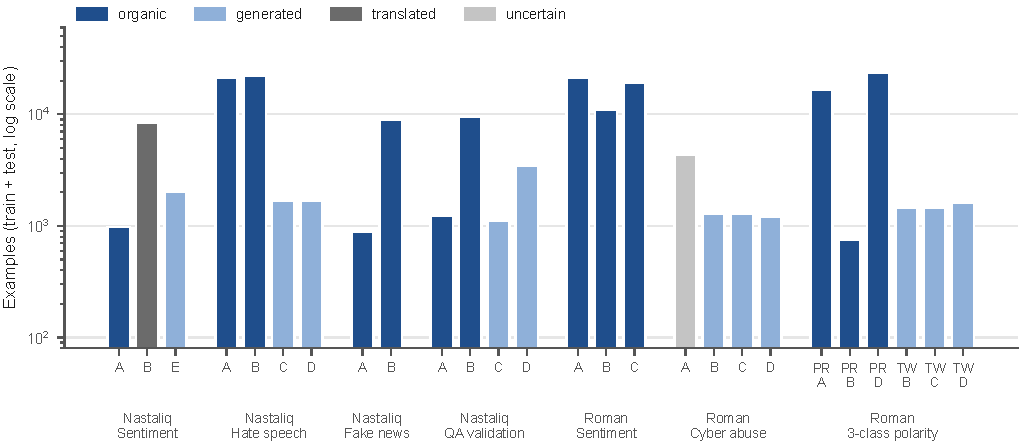
\includegraphics[width=\textwidth]{figures/overview.pdf}
\caption{Size of every domain (training and test items, log scale), grouped by transfer matrix and coloured by data origin. Exact counts and class distributions are in Table~\ref{tab:datasets}.}
\label{fig:overview}
\end{figure*}

\begin{table*}[t]
\centering\scriptsize\setlength{\tabcolsep}{3.2pt}
\caption{The benchmark. $C$: number of classes; test distribution in label order (binary: negative/normal/fake/invalid first; 3-class: negative/neutral/positive). Origin: \emph{organic} (public corpus of native text), \emph{translated} (machine-translated from English), \emph{generated} (LLM-generated, Section~\ref{sec:collection}) or \emph{uncertain}. Near-dup.\,\%: share of test items of a random split that near-duplicated a training item (character 5-gram Jaccard $\geq 0.8$). Split: \emph{random} = stratified random split with leaking items removed; \emph{cluster} = split so that near-duplicate clusters do not straddle train and test (Section~\ref{sec:splits}).}
\label{tab:datasets}
\resizebox{\textwidth}{!}{%
\begin{tabular}{llllrrrllrl}
\toprule
Script & Transfer matrix & ID & Domain & $C$ & $N_\text{train}$ & $N_\text{test}$ & Test dist. & Origin & Near-dup.\,\% & Split \\
\midrule
Nastaliq & Sentiment & SA-A & Twitter Social Media & 2 & 781 & 194 & 99/95 & organic & 1.0 & original \\
 &  & SA-B & Movie Reviews & 2 & 6,695 & 1,638 & 808/830 & translated & 0.1 & original \\
 &  & SA-E & Socioeconomic Agricultural & 2 & 1,629 & 407 & 203/204 & generated & 43.0 & cluster \\
\midrule
 & Hate Speech & HS-A & Social Media Offensive & 2 & 17,152 & 4,133 & 2452/1681 & organic & 1.8 & original \\
 &  & HS-B & Social Media Hate Speech & 2 & 18,486 & 3,540 & 1304/2236 & organic & 7.4 & original \\
 &  & HS-C & Politics Sports Health Family & 2 & 1,360 & 340 & 120/220 & generated & 27.1 & cluster \\
 &  & HS-D & Sports Labor Arts Education & 2 & 1,356 & 339 & 169/170 & generated & 38.6 & cluster \\
\midrule
 & Fake News & FN-A & Multi Topic News & 2 & 634 & 260 & 112/148 & organic & 0.0 & original \\
 &  & FN-B & Ax to Grind & 2 & 7,217 & 1,645 & 789/856 & organic & 1.2 & original \\
\midrule
 & QA Validation & QA-A & Religious Hadith & 2 & 992 & 250 & 125/125 & organic & 0.0 & original \\
 &  & QA-B & General Knowledge & 2 & 7,564 & 1,889 & 946/943 & organic & 0.2 & original \\
 &  & QA-C & Long Form QnA & 2 & 896 & 224 & 112/112 & generated & 0.0 & original \\
 &  & QA-D & Short Form QnA & 2 & 2,764 & 691 & 348/343 & generated & 0.7 & original \\
\midrule
Roman & Sentiment (binary) & SA-A & Mixed Public Discourse & 2 & 19,262 & 2,140 & 1001/1139 & organic & 0.4 & original \\
 &  & SA-B & Social Media Politics Drama & 2 & 8,781 & 2,163 & 1049/1114 & organic & 1.3 & original \\
 &  & SA-C & YouTube Entertainment & 2 & 15,587 & 3,759 & 1630/2129 & organic & 0.7 & original \\
\midrule
 & Cyber Abuse & CA-A & YouTube Comments & 2 & 3,469 & 866 & 418/448 & uncertain & 13.2 & cluster \\
 &  & CA-B & Content Creator Comments & 2 & 1,040 & 260 & 116/144 & generated & 63.5 & cluster \\
 &  & CA-C & Social Media Diverse Vocab & 2 & 1,040 & 260 & 120/140 & generated & 59.6 & cluster \\
 &  & CA-D & General Online Video & 2 & 960 & 240 & 110/130 & generated & 51.2 & cluster \\
\midrule
 & 3-class Polarity & PR-A & Daraz Ecommerce & 3 & 13,489 & 3,294 & 850/487/1957 & organic & 1.4 & original \\
 &  & PR-B & Restaurant Food & 3 & 600 & 148 & 8/23/117 & organic & 1.3 & original \\
 &  & PR-D & General Social Comments & 3 & 19,349 & 4,026 & 1380/1158/1488 & organic & 0.3 & original \\
 &  & TW-B & Consumer Electronics Gaming & 3 & 1,160 & 290 & 98/96/96 & generated & 90.7 & cluster \\
 &  & TW-C & Public Civic Services & 3 & 1,160 & 290 & 98/96/96 & generated & 88.6 & cluster \\
 &  & TW-D & Mixed Social Commentary & 3 & 1,280 & 320 & 110/103/107 & generated & 90.6 & cluster \\
\midrule
\multicolumn{5}{l}{Total (26 domains)} & 154,703 & 33,606 & & & & \\
\bottomrule
\end{tabular}}

\end{table*}

\subsection{Generated domains}\label{sec:collection}
Most task types have too few public Urdu corpora to form three or more domains. For the missing domains the first author generated data with xAI Grok. Each prompt described the target domain in detail (topic, platform, register and label definitions) and included examples from existing public datasets of the same task, and asked for new labelled items in that domain. Claude and ChatGPT were tried first and discarded because their Urdu and Roman Urdu output was judged less natural. The first author, a native Urdu speaker, read all generated items and removed or corrected unnatural or mislabelled ones. No second annotator was involved, and neither the prompts nor the number of removed items were recorded. None of the three evaluated LLMs was used for generation.

Rather than rely on a recollection of how much of each domain was generated, we measured generation signals directly (Appendix Table~\ref{tab:synth-audit}): the share of items with a near-duplicate variant inside the domain, lexical diversity, and the variability of item length. The two groups separate cleanly on length: every generated domain has a coefficient of variation of item length of at most \GenLenCVMax{}, and every organic domain at least \OrgLenCVMin{}; generated domains also reach template rates of up to \GenTemplateMax\%. The signals are uniform across each generated domain, so we treat all \NumSynthDomains{} such domains (\NumSynthRows{} examples, \PctSynth\% of the benchmark) as generated in full. The share is concentrated: generated domains are one of three in Nastaliq sentiment, two of four in hate speech and QA, three of four in Roman cyber abuse and three of six in 3-class polarity, and none in fake news or Roman binary sentiment. Roman CA-A is recorded as organic but shows augmentation-like noise (inserted emoticons, repeated punctuation, misspellings) and a 13\% near-duplicate rate, so we label it \emph{uncertain}.

\subsection{Inclusion criteria}\label{sec:criteria}
A candidate domain enters the benchmark only if it meets three criteria. Table~\ref{tab:dropped} lists the \NumDropped{} candidates that fail them.

\begin{enumerate}[leftmargin=*,itemsep=2pt]
\item \textbf{Distinct source.} A domain must not repeat the text of another domain of the same matrix. Three candidates did: an ISE-Hate Level-1 file \citep{akram2023isehate} that annotates the same tweet pool as HS-A, a political-tweet file identical to Nastaliq SA-A, and a second copy of the RUSAD corpus. Every shift between such a pair is effectively in-domain. Where only part of a domain overlapped another (e.g.\ 84\% of Nastaliq SA-A tweets also occurred in SA-B), the shared texts were removed from the larger domain.
\item \textbf{Label not predictable from origin.} A domain is excluded when its label can be read off where an item came from. Two candidates were distributed with each class taken from a different source: in one Roman opinion candidate every positive and negative item is a RUSAD review while every neutral item comes elsewhere, and in one Nastaliq fake-news candidate the fake items are largely fact-check verdicts and the real items ordinary news. To find less obvious cases we ran a \emph{single-phrase shortcut audit} on every domain: for each word n-gram ($n\leq 3$) we compute the difference between its document frequency in one class and in the others, and inspect the top phrases (Appendix Table~\ref{tab:shortcuts}). In one further fake-news candidate the dateline token ``92'' (from ``92 News'') occurs in \val{sc.N-FN.FN-D.in}\% of real items and \val{sc.N-FN.FN-D.out}\% of fake items, so a model could classify it by recognising the outlet. All three were excluded. In the included domains the highest-scoring phrases are content words, such as \textit{nahi} (``not'') for negative opinions, with one exception discussed in Section~\ref{sec:limitations}.
\item \textbf{Minimum size.} A domain needs at least 100 test items. One generated sentiment candidate had 33.
\end{enumerate}

\begin{table*}[t]
\centering\small
\caption{Candidate domains excluded by the inclusion criteria of Section~\ref{sec:criteria}.}
\label{tab:dropped}
\resizebox{\textwidth}{!}{\begin{tabular}{lllp{6.0cm}}
\toprule
Script & Collection & Domain & Reason \\
\midrule
Nastaliq & Hate Speech & Inter Faith Sectarian Ethnic & same tweets and labels as Hate Speech A (ISE Level-1 re-uses the 22K Offensive pool) \\
Nastaliq & Sentiment Analysis & Governance Political & same texts and labels as Sentiment A \\
Roman & Sentiment Analysis & Utilities Apps Courses & same 11,000-review corpus as Roman Sentiment B \\
Roman & Twitter or Social Media Opinions & Twitter Political Social & positive/negative items are the RUSAD corpus (= Roman Sentiment B); all neutral items come from a different source, so the label is predictable from the source \\
Nastaliq & Fake News Detection & General Pakistani News & fake and real items come from two separate files; fake items are largely fact-check verdicts, so the label is predictable from the source \\
Nastaliq & Fake News Detection & Fact Checking Platform & real items carry an outlet dateline (``92 News'', 90\% of real vs 3.5\% of fake items), so the label is predictable from the source \\
Nastaliq & Sentiment Analysis & Civic Social Topics & too small to evaluate (162 items, 33 in test; minimum is 100 test items) \\
\bottomrule
\end{tabular}
}
\end{table*}

\subsection{Leakage-aware splits}\label{sec:splits}
Domains distributed with an official split (Nastaliq SA-B, FN-A and Roman SA-A) keep it. The other non-QA domains were split 80/20 at random, stratified by label (seed 42), after removing test items whose text also occurred in training. Exact de-duplication is not enough for generated text. MinHash near-duplicate detection \citep{broder1997resemblance} (character 5-grams, verified Jaccard $\geq 0.8$) showed that in the generated non-QA domains 27--91\% of test items of a random split near-duplicated a training item, against at most 7\% in any organic domain except CA-A (13\%). The duplicates are the same sentence with a filler added or swapped (\textit{``\dots hain bhai''} vs.\ \textit{``\dots hain bhai ok''}), a form of train--test leakage \citep{elangovan2021memorization}. For the \NumResplit{} domains in which more than 10\% of test items leaked, near-duplicates were grouped into clusters and the domain was split 80/20 so that whole clusters fall on one side (stratified group split, seed 42); elsewhere the leaking test items were removed.

Pair tasks need a further step. A random split of question--answer pairs places the same question in training and test: in our QA domains this happened for 28--84\% of test questions. QA domains are therefore split by \emph{question group}: rows are linked when their questions are identical or near-duplicates, or when they share a distinctive answer of four or more words, and whole groups are assigned to training or test (80/20, seed 42). Pairs are then built inside each split, every question with its own answer (valid) and with an answer from a different group (invalid), so classes are balanced and no distractor answers a duplicate of the question.

After these steps no test item in any domain has an exact or near-duplicate in its training split. Fine-tuning holds out a further 10\% of the source training split, stratified by label, for early stopping (Section~\ref{sec:ft}). The build is deterministic: rebuilding under different Python hash seeds produces byte-identical files.

\subsection{Licensing and release}\label{sec:licensing}
Appendix Table~\ref{tab:provenance} lists the licence of every source. Seven sources are released under MIT, CC BY 4.0 or ODbL 1.0. Four published corpora (the Urdu Sentiment Corpus, ISE-Hate, Bend the Truth and Ax-to-Grind Urdu) are publicly available but state no licence; for these we distribute a script that downloads the original files and rebuilds our splits, unless the authors grant permission to redistribute. Generated domains are released with attribution to xAI Grok, as its terms of service request. The three untraced domains have no identifiable licence; we release them for research use and will remove any of them on request from a rights holder. The splits, build scripts, audits, model predictions and prompts are available at \repo{} and on Zenodo.

% =====================================================================
\section{Methodology}\label{sec:method}

\subsection{Evaluation design}
For every matrix with domains $D_1,\dots,D_n$ we train (or prompt) one model per source domain $D_i$ and evaluate it on the test split of every domain $D_j$ of the matrix, filling an $n\times n$ matrix of macro-F1 scores $F(i\to j)$. The diagonal gives in-domain performance and the off-diagonal cells give the \NumShifts{} cross-domain shifts across the seven matrices. Transfer is evaluated only inside a matrix, where the label space is identical, and scores are never pooled across scripts.

\subsection{Metrics}\label{sec:metrics}
All scores are macro-averaged F1 over the $C$ classes of the matrix, $\text{F1}_\text{macro}=\frac{1}{C}\sum_{c}\frac{2P_cR_c}{P_c+R_c}$, which weights minority classes equally and is needed for the imbalanced abusive-language and fake-news domains. Following \citet{calderon2024measuring}, for a shift $(i,j)$:
\begin{align}
\text{SS}_i &= F(i\to i), \qquad \text{TT}_j = F(j\to j),\\
\text{ST}_{ij} &= F(i\to j),\\
\dS(i,j) &= \text{SS}_i - \text{ST}_{ij},\\
\dT(i,j) &= \text{TT}_j - \text{ST}_{ij}.
\end{align}
The Source Drop $\dS$ measures how much a model loses when it is moved away from its own domain; the Target Drop $\dT$ measures how far it falls short of a model trained on the target itself. A shift with $\dS>0$ but $\dT\le 0$ is a move to a \emph{harder} target: the source model does as well there as the target's own model, so the loss reflects target difficulty rather than a robustness failure.

Averaged over all $n(n-1)$ shifts of a complete matrix, $\overline{\dS}=\overline{\dT}$ exactly, because each domain is a source in $n-1$ shifts and a target in $n-1$ shifts. A matrix-level mean Target Drop therefore adds nothing to the mean Source Drop. The Target Drop is informative \emph{per shift} and \emph{per target domain}, and we report it in three ways: the worst-case drops over shifts, $\text{WSD}=\max_{i\neq j}\dS(i,j)$ and $\text{WTD}=\max_{i\neq j}\dT(i,j)$; the percentage of shifts with a positive Target Drop and the percentage of harder-target shifts; and, per target domain $j$, $\text{TT}_j$ with the mean $\dT$ over all sources (Tables~\ref{tab:pertarget-n} and~\ref{tab:pertarget-r}).

\paragraph{Relative robustness.} $\%\text{Rob}=100\cdot\overline{\text{ST}}/\overline{\text{SS}}$ is the share of in-domain performance retained across domains. Drops are reported in percentage points (pp) of macro-F1, and every claim about \%Rob is accompanied by the absolute ST it is computed from.

\subsection{Baselines and degeneracy guards}\label{sec:guard}
Every results table includes a majority-class baseline (the macro-F1 of always predicting the target's most frequent class) and a uniform-random baseline (its expected macro-F1, $\frac{1}{C}\sum_c \frac{2p_c/C}{p_c+1/C}$ for class priors $p_c$), each averaged over the target domains. It also includes a \emph{length-only} shortcut baseline: a logistic regression on the logarithms of an item's character and word counts, trained on each source domain and evaluated on every target exactly like the models. In a matrix in which this baseline performs well, labels are partly predictable from length, and a model's advantage over it is the part of its performance that length cannot explain.

A model near the floor of the metric has little to lose, so its $\%\text{Rob}$ approaches 100\% without reflecting robustness. Two guards address this. First, $\%\text{Rob}$ is suppressed (n/a$^\dagger$) when $\overline{\text{SS}}$ is less than 0.05 above the uniform-random baseline, and whenever $\%\text{Rob}\geq 100\%$. Second, $\%\text{Rob}$ is marked $^\ddagger$ when $\overline{\text{SS}}$ does not exceed the in-domain score of the length-only baseline, because such a model has not shown that it learned more than text length.

\subsection{Fine-tuned encoders}\label{sec:ft}
We fine-tune XLM-R base (\nolinkurl{xlm-roberta-base}, 278M parameters) \citep{conneau2020xlmr} and mBERT (\nolinkurl{bert-base-multilingual-cased}, 178M) \citep{devlin2019bert} with a linear classification head using Hugging Face Transformers \citep{wolf2020transformers}. Training data per source is capped at 8{,}000 examples by stratified sampling (fixed across seeds), and 10\% is held out for validation. We use AdamW with learning rate $2\times10^{-5}$, linear warm-up over 10\% of steps, weight decay 0.01, batch size 16, at most 5 epochs, and early stopping with patience 2 on validation macro-F1, keeping the best epoch. Inputs are truncated to 128 tokens, or 256 for fake news and QA; QA pairs are encoded as sentence pairs. Each configuration is run with three seeds (13, 42, 87), which vary initialisation, data order and the validation split \citep{dodge2020finetuning,mosbach2021stability}. Training depends only on the source domain, so each (model, seed, source) is trained once and evaluated on every target of its matrix. Hyperparameters were fixed in advance and not tuned per domain.

\subsection{Few-shot LLMs}\label{sec:llm}
We evaluate Llama-3.1-8B-Instruct \citep{grattafiori2024llama3}, Qwen2.5-7B-Instruct \citep{qwen2024qwen25} and Mistral-7B-Instruct-v0.3 \citep{jiang2023mistral}, loaded with 4-bit NF4 quantisation \citep{dettmers2023qlora}. The prompt (Appendix~\ref{app:prompt}), formatted with each model's chat template, states the task and script, lists the allowed labels, and gives five demonstrations per class sampled from the source training split and shuffled; the test item follows. Each text in the prompt is truncated to the same token budget as the encoders, so the test item is never cut from the prompt. Decoding is greedy with at most six new tokens. The prediction is the earliest whole-word label name in the output; outputs that name no label are counted as errors and reported as the parse-failure rate. Every configuration is repeated with three demonstration draws (seeds 13, 42, 87). LLMs are evaluated on a fixed stratified sample of up to 300 test items per target domain, identical across sources, models and seeds; whenever the two families are compared directly, fine-tuned predictions are restricted to the same items.

\paragraph{In-domain means something different for the two families.} For a fine-tuned model, SS versus ST contrasts learned weights applied inside and outside their training distribution. For a few-shot LLM the weights never change: SS versus ST contrasts demonstrations drawn from the target domain with demonstrations drawn from another domain. The two relative-robustness figures therefore answer different questions (sensitivity to the training data versus sensitivity to the source of the demonstrations), and the two families also see very different amounts of source data (up to 8{,}000 training items against ten or fifteen demonstrations). Following \citet{calderon2024measuring}, we compare them as two practical ways of building a classifier from source-domain data, not as a like-for-like measurement of one mechanism.

\subsection{Variance and significance}\label{sec:stats}
Every aggregate is computed per seed and reported as mean $\pm$ standard deviation over the three seeds (or demonstration draws). Differences between a fine-tuned model and an LLM are tested with a paired bootstrap \citep{koehn2004significance,dror2018hitchhiker}: test items are resampled with replacement within each target domain, the same resample is applied to both systems, and mean ST (averaged over seeds and shifts) is recomputed 5{,}000 times. We report 95\% confidence intervals and two-sided $p$-values, and because the \val{boot.n} comparisons form one family of tests, we control the family-wise error rate with the Holm--Bonferroni procedure. A difference is called significant only when its Holm-adjusted $p$ is below 0.05. Differences between models of the same family are not tested and are described only as numbers.

\subsection{Control for synthetic data}\label{sec:organic-method}
To test whether generated domains drive the conclusions (RQ4), we recompute every aggregate on the submatrix of \emph{organic} domains (native Urdu text from public corpora, excluding generated, machine-translated and uncertain domains) for each matrix that retains at least two of them.

% =====================================================================
\section{Experimental setup}\label{sec:setup}
All experiments ran on one workstation: Intel Core i7-13700 (16 cores), 32\,GB RAM, NVIDIA RTX A4000 (16\,GB), PyTorch 2.14 with CUDA 12.6, Transformers 4.57 and bitsandbytes 0.50. The evaluation comprises \val{compute.ftruns} fine-tuning runs (two encoders, three seeds, \NumDomains{} source domains), which produce \val{compute.ftcells} scored matrix cells, and \val{compute.llmcells} LLM matrix cells (three models, three demonstration draws). Fine-tuning took \val{compute.fthours} GPU-hours of training and LLM inference \val{compute.llmhours} GPU-hours. To make LLM inference feasible, the prompt prefix shared by all test items of a (source, demonstration draw) pair is encoded once and its attention cache reused. On a check of 32 fake-news items per model, predictions with and without the cache agreed on all 96 items.

% =====================================================================
\section{Results}\label{sec:results}
Figure~\ref{fig:ssst} summarises in-domain and cross-domain scores for every model and matrix; Tables~\ref{tab:res-nsa}--\ref{tab:res-rp3} give the full aggregates, Figures~\ref{fig:mat-n} and~\ref{fig:mat-r} the transfer matrices, and Figure~\ref{fig:forest} the paired tests between the two families.

\begin{figure*}[t]
\centering
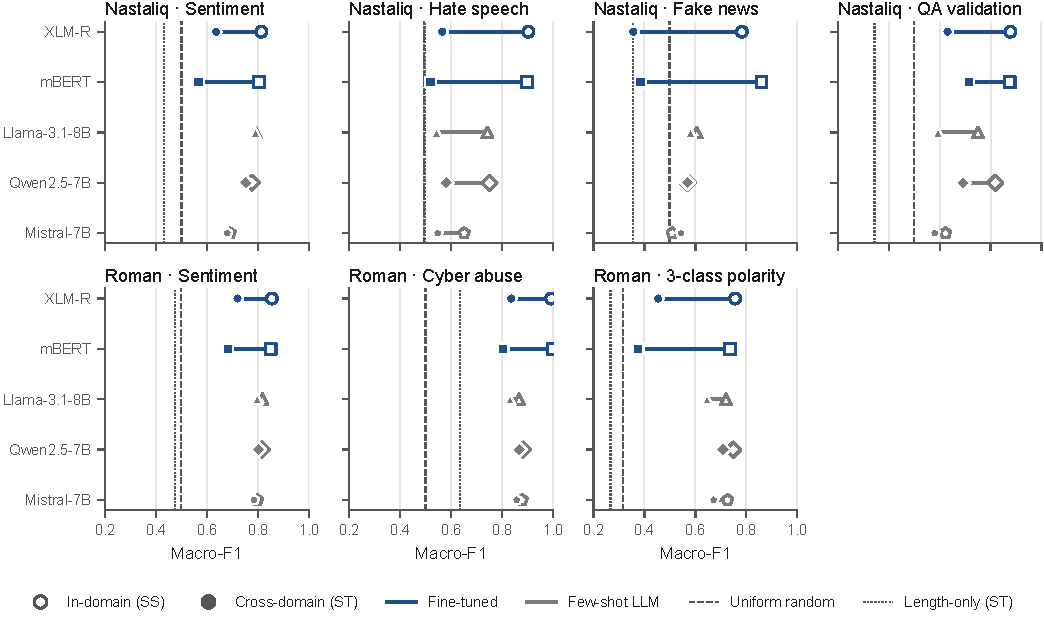
\includegraphics[width=\textwidth]{figures/ss_st.pdf}
\caption{In-domain (open markers) and cross-domain (filled markers) macro-F1 for every model and matrix, as means over three seeds or demonstration draws; the line between the two markers is the mean Source Drop. Blue: fine-tuned encoders; orange: few-shot LLMs; marker shape identifies the model. Seed standard deviations are in Tables~\ref{tab:res-nsa}--\ref{tab:res-rp3}. Dashed line: uniform-random baseline; dotted line: cross-domain score of the length-only baseline.}
\label{fig:ssst}
\end{figure*}

\subsection{Nastaliq track}\label{sec:res-n}
\paragraph{Sentiment (Table~\ref{tab:res-nsa}).} The encoders reach SS of \val{N-SA.XLM-R.SS}\,$\pm$\,\val{N-SA.XLM-R.SSsd} (XLM-R) and \val{N-SA.mBERT.SS}\,$\pm$\,\val{N-SA.mBERT.SSsd} (mBERT) and keep \val{range.N-SA.ft.rob}\% of it across domains (ST \val{range.N-SA.ft.ST}). The LLMs score slightly lower in-domain (SS \val{range.N-SA.llm.SS}) but lose almost nothing (ST \val{range.N-SA.llm.ST}). XLM-R's cross-domain score varies across seeds (SD \val{N-SA.XLM-R.STsd}), mostly on shifts into the translated movie reviews.

\paragraph{Hate speech (Table~\ref{tab:res-nhs}).} The encoders score SS \val{range.N-HS.ft.SS} but ST only \val{range.N-HS.ft.ST}, a mean Source Drop of \val{range.N-HS.ft.dS} pp and a worst single-shift Target Drop of \val{N-HS.XLM-R.WTD} pp for XLM-R. The LLMs are weaker in-domain (SS \val{range.N-HS.llm.SS}) and reach ST \val{range.N-HS.llm.ST}. Across domains XLM-R does not differ significantly from any LLM, whereas mBERT is significantly below all three, by $\val{boot.N-HS.mBERT.Llama-3.1-8B.diff}$ to $\val{boot.N-HS.mBERT.Qwen2.5-7B.diff}$ pp. Apart from QA, hate speech is the Nastaliq matrix with the smallest difference between the families.

\paragraph{Fake news (Table~\ref{tab:res-nfn}).} Fine-tuned encoders fit each fake-news domain (SS \val{N-FN.XLM-R.SS}\,$\pm$\,\val{N-FN.XLM-R.SSsd} for XLM-R, \val{N-FN.mBERT.SS}\,$\pm$\,\val{N-FN.mBERT.SSsd} for mBERT) but transfer below chance: ST is \val{range.N-FN.ft.ST}, against a uniform-random baseline of \val{N-FN.rand} and a length-only cross-domain score of \val{N-FN.Length-only.ST}. XLM-R's high seed variance comes from FN-A, whose training split has 634 items. Among the LLMs only Llama-3.1-8B clears both the random and the length-only baseline in-domain (SS \val{N-FN.Llama-3.1-8B.SS} against \val{N-FN.lenSS}); Qwen2.5-7B and Mistral-7B do not, and their \%Rob is suppressed. Llama-3.1-8B's cross-domain score (\val{N-FN.Llama-3.1-8B.ST}) is significantly higher than that of both encoders (Figure~\ref{fig:forest}), but it is still close to chance. Neither family provides a fake-news classifier that transfers between these two corpora.

\paragraph{QA pair validation (Table~\ref{tab:res-nqa}).} QA is the one matrix in which fine-tuning also wins across domains. The encoders reach SS \val{range.N-QA.ft.SS} and ST \val{range.N-QA.ft.ST}, and both exceed Llama-3.1-8B (ST \val{N-QA.Llama-3.1-8B.ST}) and Mistral-7B (ST \val{N-QA.Mistral-7B.ST}) significantly, by $\val{boot.N-QA.XLM-R.Llama-3.1-8B.diff}$ to $\val{boot.N-QA.mBERT.Mistral-7B.diff}$ pp. Qwen2.5-7B (SS \val{N-QA.Qwen2.5-7B.SS}, ST \val{N-QA.Qwen2.5-7B.ST}) is significantly above XLM-R ($\val{boot.N-QA.XLM-R.Qwen2.5-7B.diff}$ pp, \val{boot.N-QA.XLM-R.Qwen2.5-7B.p}) and does not differ significantly from mBERT. The length-only baseline is at chance (SS \val{N-QA.lenSS}), as expected for balanced pairs whose distractors come from the same domain.

\subsection{Roman Urdu track}\label{sec:res-r}
\paragraph{Sentiment, binary (Table~\ref{tab:res-rsa}).} The encoders are close in-domain (SS \val{R-SA.XLM-R.SS} and \val{R-SA.mBERT.SS}) and lose \val{range.R-SA.ft.dS} pp across domains (ST \val{range.R-SA.ft.ST}). The LLMs are slightly weaker in-domain (SS \val{range.R-SA.llm.SS}) and lose \val{range.R-SA.llm.dS} pp, so their ST (\val{range.R-SA.llm.ST}) is significantly higher than that of both encoders in all six comparisons ($\val{boot.R-SA.XLM-R.Mistral-7B.diff}$ to $\val{boot.R-SA.mBERT.Qwen2.5-7B.diff}$ pp).

\paragraph{Cyber abuse (Table~\ref{tab:res-rca}).} In-domain scores are close to perfect for the encoders (SS \val{R-CA.XLM-R.SS} and \val{R-CA.mBERT.SS}), and ST is \val{range.R-CA.ft.ST}. No test item has a near-duplicate in training, so the high in-domain scores are not caused by leakage; they indicate that these domains are easy to fit, which is consistent with the uniform style of the three generated domains and the augmentation-like noise of CA-A. The length-only baseline reaches SS \val{R-CA.lenSS} and ST \val{R-CA.Length-only.ST}, the highest of any matrix. XLM-R does not differ significantly from any LLM across domains; mBERT is significantly below Qwen2.5-7B and Mistral-7B.

\paragraph{3-class polarity (Table~\ref{tab:res-rp3}).} This matrix has the largest fine-tuned losses in the Roman track: SS \val{range.R-P3.ft.SS}, ST \val{range.R-P3.ft.ST}, a mean Source Drop of \val{range.R-P3.ft.dS} pp and a worst Target Drop of \val{R-P3.XLM-R.WTD} pp (XLM-R). The LLMs have similar in-domain scores (SS \val{range.R-P3.llm.SS}) but keep them (ST \val{range.R-P3.llm.ST}), and their advantage over the encoders is the largest in the study, from $\val{boot.R-P3.XLM-R.Llama-3.1-8B.diff}$ to $\val{boot.R-P3.mBERT.Qwen2.5-7B.diff}$ pp, significant in all six comparisons.

\begin{figure*}[t]
\centering
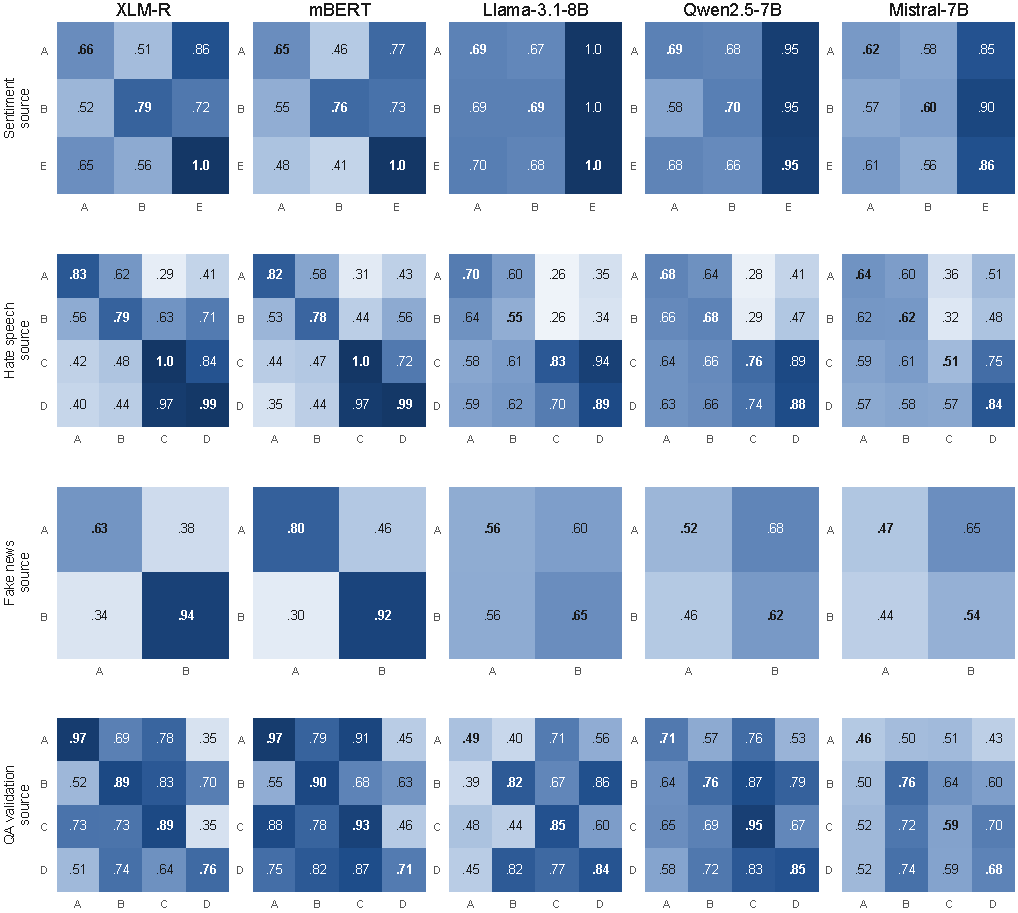
\includegraphics[width=\textwidth]{figures/matrices_nastaliq.pdf}
\caption{Nastaliq transfer matrices: macro-F1 of a model trained or prompted on the row domain and tested on the column domain, mean over three seeds or demonstration draws. The diagonal (bold) is in-domain performance; darker cells are higher.}
\label{fig:mat-n}
\end{figure*}

\begin{figure*}[t]
\centering
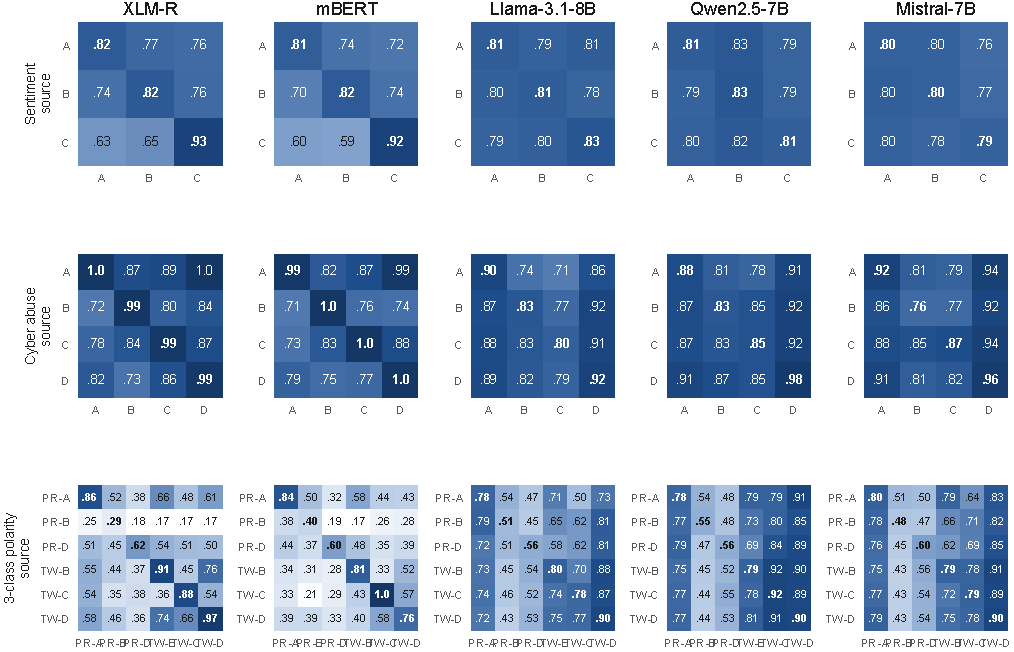
\includegraphics[width=\textwidth]{figures/matrices_roman.pdf}
\caption{Roman Urdu transfer matrices; layout as in Figure~\ref{fig:mat-n}.}
\label{fig:mat-r}
\end{figure*}

\begin{table*}[t]\centering\small
\caption{Nastaliq Sentiment (3 domains, 6 shifts). Macro-F1, mean$\pm$SD over 3 seeds (fine-tuned) or 3 demonstration draws (LLMs). $\overline{\Delta_S}$, WSD and WTD in pp; $\Delta_T{>}0$\,\%: share of shifts with positive Target Drop; Harder-tgt\,\%: share with $\Delta_S>0$ and $\Delta_T\le 0$. $^\dagger$: \%Rob suppressed (SS within 0.05 of random, or \%Rob $\geq$ 100); $^\ddagger$: SS not above the length-only baseline (Section~\ref{sec:guard}). Drops and \%Rob are computed from unrounded scores, so they can differ by 0.1 from differences of the displayed values.}
\label{tab:res-nsa}\resizebox{\textwidth}{!}{\begin{tabular}{lcccccccc}
\toprule
Model & SS & ST & $\overline{\Delta_S}$ & WSD & WTD & $\Delta_T{>}0$\,\% & Harder-tgt\,\% & \%Rob \\
\midrule
Majority class & 0.336 & -- & -- & -- & -- & -- & -- & -- \\
Uniform random & 0.500 & -- & -- & -- & -- & -- & -- & -- \\
Length-only (shortcut) & 0.552 & 0.432 & 11.9 & 27.0 & 21.3 & 100.0 & 0.0 & 78.4 \\
\midrule
XLM-R (fine-tuned) & 0.813\,$\pm$\,0.011 & 0.636\,$\pm$\,0.074 & 17.8 & 43.3 & 33.7 & 94.4 & 5.6 & 78.1 \\
mBERT (fine-tuned) & 0.805\,$\pm$\,0.003 & 0.567\,$\pm$\,0.008 & 23.7 & 58.8 & 35.3 & 100.0 & 0.0 & 70.5 \\
\midrule
Llama-3.1-8B (few-shot) & 0.792\,$\pm$\,0.024 & 0.790\,$\pm$\,0.010 & 0.2 & 32.2 & 3.4 & 44.4 & 22.2 & 99.8 \\
Qwen2.5-7B (few-shot) & 0.777\,$\pm$\,0.011 & 0.752\,$\pm$\,0.009 & 2.5 & 28.7 & 10.6 & 72.2 & 0.0 & 96.8 \\
Mistral-7B (few-shot) & 0.691\,$\pm$\,0.019 & 0.679\,$\pm$\,0.018 & 1.2 & 30.2 & 6.5 & 66.7 & 11.1 & 98.3 \\
\bottomrule
\end{tabular}
}
\end{table*}
\begin{table*}[t]\centering\small
\caption{Nastaliq Hate Speech (4 domains, 12 shifts). Columns as in Table~\ref{tab:res-nsa}.}
\label{tab:res-nhs}\resizebox{\textwidth}{!}{\begin{tabular}{lcccccccc}
\toprule
Model & SS & ST & $\overline{\Delta_S}$ & WSD & WTD & $\Delta_T{>}0$\,\% & Harder-tgt\,\% & \%Rob \\
\midrule
Majority class & 0.372 & -- & -- & -- & -- & -- & -- & -- \\
Uniform random & 0.494 & -- & -- & -- & -- & -- & -- & -- \\
Length-only (shortcut) & 0.595 & 0.494 & 10.0 & 24.6 & 29.2 & 83.3 & 8.3 & 83.1 \\
\midrule
XLM-R (fine-tuned) & 0.903\,$\pm$\,0.004 & 0.565\,$\pm$\,0.002 & 33.8 & 58.9 & 70.8 & 100.0 & 0.0 & 62.6 \\
mBERT (fine-tuned) & 0.897\,$\pm$\,0.003 & 0.519\,$\pm$\,0.007 & 37.8 & 64.9 & 69.2 & 100.0 & 0.0 & 57.9 \\
\midrule
Llama-3.1-8B (few-shot) & 0.742\,$\pm$\,0.027 & 0.542\,$\pm$\,0.002 & 20.0 & 44.3 & 59.5 & 80.6 & 13.9 & 73.1 \\
Qwen2.5-7B (few-shot) & 0.750\,$\pm$\,0.007 & 0.581\,$\pm$\,0.005 & 16.9 & 40.4 & 50.2 & 88.9 & 5.6 & 77.5 \\
Mistral-7B (few-shot) & 0.651\,$\pm$\,0.006 & 0.548\,$\pm$\,0.017 & 10.3 & 32.3 & 36.4 & 80.6 & 13.9 & 84.1 \\
\bottomrule
\end{tabular}
}
\end{table*}
\begin{table*}[t]\centering\small
\caption{Nastaliq Fake News (2 domains, 2 shifts). Columns as in Table~\ref{tab:res-nsa}.}
\label{tab:res-nfn}\resizebox{\textwidth}{!}{\begin{tabular}{lcccccccc}
\toprule
Model & SS & ST & $\overline{\Delta_S}$ & WSD & WTD & $\Delta_T{>}0$\,\% & Harder-tgt\,\% & \%Rob \\
\midrule
Majority class & 0.353 & -- & -- & -- & -- & -- & -- & -- \\
Uniform random & 0.499 & -- & -- & -- & -- & -- & -- & -- \\
Length-only (shortcut) & 0.570 & 0.354 & 21.5 & 26.9 & 29.3 & 100.0 & 0.0 & 62.2 \\
\midrule
XLM-R (fine-tuned) & 0.782\,$\pm$\,0.119 & 0.356\,$\pm$\,0.030 & 42.6 & 60.0 & 55.9 & 100.0 & 0.0 & 45.9 \\
mBERT (fine-tuned) & 0.860\,$\pm$\,0.008 & 0.384\,$\pm$\,0.005 & 47.6 & 61.8 & 49.5 & 100.0 & 0.0 & 44.7 \\
\midrule
Llama-3.1-8B (few-shot) & 0.605\,$\pm$\,0.061 & 0.581\,$\pm$\,0.022 & 2.4 & 9.1 & 7.6 & 50.0 & 33.3 & 96.4 \\
Qwen2.5-7B (few-shot) & 0.570\,$\pm$\,0.054 & 0.569\,$\pm$\,0.021 & 0.1 & 15.5 & 6.3 & 66.7 & 0.0 & n/a$^\dagger$ \\
Mistral-7B (few-shot) & 0.509\,$\pm$\,0.042 & 0.543\,$\pm$\,0.023 & -3.5 & 10.6 & 3.7 & 50.0 & 0.0 & n/a$^\dagger$ \\
\bottomrule
\end{tabular}
}
\end{table*}
\begin{table*}[t]\centering\small
\caption{Nastaliq QA Pair Validation (4 domains, 12 shifts). Columns as in Table~\ref{tab:res-nsa}.}
\label{tab:res-nqa}\resizebox{\textwidth}{!}{\begin{tabular}{lcccccccc}
\toprule
Model & SS & ST & $\overline{\Delta_S}$ & WSD & WTD & $\Delta_T{>}0$\,\% & Harder-tgt\,\% & \%Rob \\
\midrule
Majority class & 0.334 & -- & -- & -- & -- & -- & -- & -- \\
Uniform random & 0.500 & -- & -- & -- & -- & -- & -- & -- \\
Length-only (shortcut) & 0.422 & 0.345 & 7.7 & 18.0 & 17.9 & 50.0 & 41.7 & n/a$^\dagger$ \\
\midrule
XLM-R (fine-tuned) & 0.878\,$\pm$\,0.017 & 0.631\,$\pm$\,0.010 & 24.7 & 62.0 & 53.4 & 94.4 & 2.8 & 71.9 \\
mBERT (fine-tuned) & 0.876\,$\pm$\,0.008 & 0.715\,$\pm$\,0.009 & 16.0 & 53.1 & 41.4 & 100.0 & 0.0 & 81.7 \\
\midrule
Llama-3.1-8B (few-shot) & 0.751\,$\pm$\,0.009 & 0.594\,$\pm$\,0.059 & 15.7 & 46.4 & 44.3 & 80.6 & 13.9 & 79.2 \\
Qwen2.5-7B (few-shot) & 0.818\,$\pm$\,0.013 & 0.692\,$\pm$\,0.032 & 12.6 & 33.0 & 31.5 & 97.2 & 0.0 & 84.6 \\
Mistral-7B (few-shot) & 0.623\,$\pm$\,0.020 & 0.581\,$\pm$\,0.012 & 4.2 & 25.9 & 27.7 & 52.8 & 36.1 & 93.3 \\
\bottomrule
\end{tabular}
}
\end{table*}
\begin{table*}[t]\centering\small
\caption{Roman Sentiment, binary (3 domains, 6 shifts). Columns as in Table~\ref{tab:res-nsa}.}
\label{tab:res-rsa}\resizebox{\textwidth}{!}{\begin{tabular}{lcccccccc}
\toprule
Model & SS & ST & $\overline{\Delta_S}$ & WSD & WTD & $\Delta_T{>}0$\,\% & Harder-tgt\,\% & \%Rob \\
\midrule
Majority class & 0.350 & -- & -- & -- & -- & -- & -- & -- \\
Uniform random & 0.499 & -- & -- & -- & -- & -- & -- & -- \\
Length-only (shortcut) & 0.600 & 0.475 & 12.5 & 24.3 & 21.1 & 100.0 & 0.0 & 79.1 \\
\midrule
XLM-R (fine-tuned) & 0.855\,$\pm$\,0.000 & 0.720\,$\pm$\,0.005 & 13.5 & 29.7 & 18.7 & 100.0 & 0.0 & 84.2 \\
mBERT (fine-tuned) & 0.850\,$\pm$\,0.003 & 0.682\,$\pm$\,0.009 & 16.8 & 34.3 & 23.2 & 100.0 & 0.0 & 80.2 \\
\midrule
Llama-3.1-8B (few-shot) & 0.818\,$\pm$\,0.011 & 0.798\,$\pm$\,0.006 & 2.0 & 4.4 & 5.0 & 88.9 & 5.6 & 97.5 \\
Qwen2.5-7B (few-shot) & 0.817\,$\pm$\,0.015 & 0.802\,$\pm$\,0.007 & 1.5 & 5.2 & 2.9 & 88.9 & 0.0 & 98.2 \\
Mistral-7B (few-shot) & 0.798\,$\pm$\,0.021 & 0.785\,$\pm$\,0.023 & 1.3 & 5.4 & 3.8 & 77.8 & 16.7 & 98.3 \\
\bottomrule
\end{tabular}
}
\end{table*}
\begin{table*}[t]\centering\small
\caption{Roman Cyber Abuse (4 domains, 12 shifts). Columns as in Table~\ref{tab:res-nsa}.}
\label{tab:res-rca}\resizebox{\textwidth}{!}{\begin{tabular}{lcccccccc}
\toprule
Model & SS & ST & $\overline{\Delta_S}$ & WSD & WTD & $\Delta_T{>}0$\,\% & Harder-tgt\,\% & \%Rob \\
\midrule
Majority class & 0.350 & -- & -- & -- & -- & -- & -- & -- \\
Uniform random & 0.499 & -- & -- & -- & -- & -- & -- & -- \\
Length-only (shortcut) & 0.770 & 0.635 & 13.5 & 25.3 & 34.2 & 83.3 & 8.3 & 82.5 \\
\midrule
XLM-R (fine-tuned) & 0.992\,$\pm$\,0.008 & 0.836\,$\pm$\,0.003 & 15.7 & 27.7 & 27.9 & 91.7 & 0.0 & 84.2 \\
mBERT (fine-tuned) & 0.998\,$\pm$\,0.001 & 0.804\,$\pm$\,0.014 & 19.4 & 28.9 & 28.5 & 100.0 & 0.0 & 80.6 \\
\midrule
Llama-3.1-8B (few-shot) & 0.866\,$\pm$\,0.023 & 0.831\,$\pm$\,0.031 & 3.4 & 19.8 & 17.1 & 66.7 & 19.4 & 96.0 \\
Qwen2.5-7B (few-shot) & 0.883\,$\pm$\,0.022 & 0.867\,$\pm$\,0.017 & 1.6 & 13.4 & 9.6 & 58.3 & 27.8 & 98.2 \\
Mistral-7B (few-shot) & 0.879\,$\pm$\,0.048 & 0.857\,$\pm$\,0.053 & 2.2 & 16.5 & 12.4 & 80.6 & 16.7 & 97.5 \\
\bottomrule
\end{tabular}
}
\end{table*}
\begin{table*}[t]\centering\small
\caption{Roman 3-class Polarity: reviews and social-media opinions (6 domains, 30 shifts). Columns as in Table~\ref{tab:res-nsa}.}
\label{tab:res-rp3}\resizebox{\textwidth}{!}{\begin{tabular}{lcccccccc}
\toprule
Model & SS & ST & $\overline{\Delta_S}$ & WSD & WTD & $\Delta_T{>}0$\,\% & Harder-tgt\,\% & \%Rob \\
\midrule
Majority class & 0.205 & -- & -- & -- & -- & -- & -- & -- \\
Uniform random & 0.316 & -- & -- & -- & -- & -- & -- & -- \\
Length-only (shortcut) & 0.385 & 0.266 & 11.8 & 28.4 & 37.7 & 90.0 & 0.0 & 69.2 \\
\midrule
XLM-R (fine-tuned) & 0.756\,$\pm$\,0.005 & 0.454\,$\pm$\,0.020 & 30.2 & 62.0 & 80.3 & 83.3 & 16.7 & 60.0 \\
mBERT (fine-tuned) & 0.736\,$\pm$\,0.011 & 0.376\,$\pm$\,0.016 & 36.0 & 79.5 & 75.4 & 93.3 & 6.7 & 51.0 \\
\midrule
Llama-3.1-8B (few-shot) & 0.720\,$\pm$\,0.011 & 0.645\,$\pm$\,0.023 & 7.5 & 46.7 & 28.7 & 87.8 & 7.8 & 89.6 \\
Qwen2.5-7B (few-shot) & 0.749\,$\pm$\,0.009 & 0.708\,$\pm$\,0.003 & 4.0 & 47.2 & 13.1 & 80.0 & 11.1 & 94.6 \\
Mistral-7B (few-shot) & 0.726\,$\pm$\,0.003 & 0.672\,$\pm$\,0.007 & 5.4 & 47.2 & 19.3 & 90.0 & 5.6 & 92.5 \\
\bottomrule
\end{tabular}
}
\end{table*}

% =====================================================================
\section{Analysis and discussion}\label{sec:analysis}

\subsection{Robustness failures or harder targets? (RQ1)}\label{sec:td}
Figure~\ref{fig:drops} plots the Source Drop of every shift against its Target Drop. For the fine-tuned encoders, \val{all.ft.posdTmin}--\val{all.ft.posdTmax}\% of shifts per matrix have a positive Target Drop, and at most \val{all.ft.hardermax}\% are harder-target shifts. Their Source Drops of \val{all.ft.dSmin}--\val{all.ft.dSmax} pp are therefore not explained by moving to difficult domains: in almost every shift, a model trained on the target does better there.

The per-target view (Tables~\ref{tab:pertarget-n} and~\ref{tab:pertarget-r}) makes this concrete for hate speech and fake news. XLM-R trained on the generated HS-C or HS-D scores TT of \val{pt.N-HS.XLM-R.HS-C.TT} and \val{pt.N-HS.XLM-R.HS-D.TT} on its own domain, while models from the other sources fall short by \val{pt.N-HS.XLM-R.HS-C.dT} and \val{pt.N-HS.XLM-R.HS-D.dT} pp on average. XLM-R trained on FN-B scores \val{pt.N-FN.XLM-R.FN-B.TT} there, and the FN-A model falls short by \val{pt.N-FN.XLM-R.FN-B.dT} pp. These targets are not intrinsically hard; the source models fail on them, which indicates that each model learns cues specific to its own source.

One target behaves differently. On Roman PR-B, XLM-R's own TT is \val{pt.R-P3.XLM-R.PR-B.TT}, below the random baseline of the matrix, and models from other sources do better there (mean $\dT$ \val{pt.R-P3.XLM-R.PR-B.dT} pp). Its test split has 8 negative items out of 148, and its training split is similarly skewed, so PR-B is a hard target for reasons of class balance rather than content; it accounts for most of the harder-target shifts of the fine-tuned models.

For the LLMs the picture is flatter, with \val{all.llm.posdTmin}--\val{all.llm.posdTmax}\% of shifts with a positive Target Drop and up to \val{all.llm.hardermax}\% harder-target shifts. Their largest per-target drops fall on the generated hate-speech domains (HS-C: \val{pt.N-HS.Llama-3.1-8B.HS-C.dT} pp for Llama-3.1-8B, \val{pt.N-HS.Qwen2.5-7B.HS-C.dT} pp for Qwen2.5-7B), where demonstrations from the target itself are needed to convey what the domain counts as hateful (Section~\ref{sec:errors}).

\begin{figure*}[t]
\centering
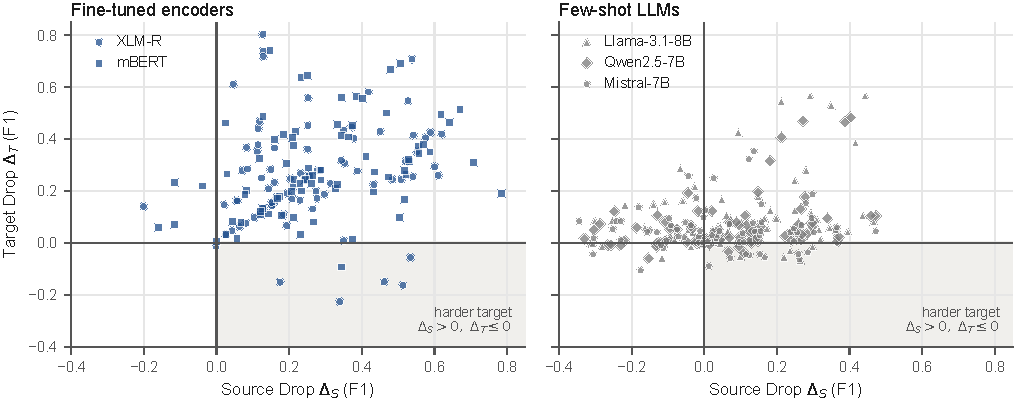
\includegraphics[width=\textwidth]{figures/source_vs_target_drop.pdf}
\caption{Source Drop against Target Drop for every shift (one point per shift and model, means over seeds). Points in the shaded lower-right region are harder-target shifts: the source model loses performance but matches or beats the target's own model.}
\label{fig:drops}
\end{figure*}

\begin{table*}[t]\centering\scriptsize\setlength{\tabcolsep}{4pt}
\caption{Per-target in-domain score TT$_j$ and mean Target Drop $\overline{\Delta_T}$ (pp, mean over all source domains) for the Nastaliq matrices. A negative $\overline{\Delta_T}$ means that models from other domains do better on the target than its own model.}
\label{tab:pertarget-n}\resizebox{\textwidth}{!}{\begin{tabular}{lrrrrrrrrrr}
\toprule
Target & \multicolumn{2}{c}{XLM-R} & \multicolumn{2}{c}{mBERT} & \multicolumn{2}{c}{Llama-3.1-8B} & \multicolumn{2}{c}{Qwen2.5-7B} & \multicolumn{2}{c}{Mistral-7B} \\
\cmidrule(lr){2-3}\cmidrule(lr){4-5}\cmidrule(lr){6-7}\cmidrule(lr){8-9}\cmidrule(lr){10-11}
 & TT & $\overline{\Delta_T}$ & TT & $\overline{\Delta_T}$ & TT & $\overline{\Delta_T}$ & TT & $\overline{\Delta_T}$ & TT & $\overline{\Delta_T}$ \\
\midrule
\multicolumn{11}{l}{\textit{Sentiment}} \\
SA-A & 0.655 & 7.0 & 0.650 & 13.4 & 0.685 & -1.1 & 0.689 & 5.8 & 0.618 & 2.6 \\
SA-B & 0.789 & 25.4 & 0.763 & 32.8 & 0.692 & 1.7 & 0.696 & 2.5 & 0.597 & 2.7 \\
SA-E & 0.997 & 20.9 & 1.000 & 24.9 & 0.998 & -0.1 & 0.946 & -0.8 & 0.859 & -1.7 \\
\midrule
\multicolumn{11}{l}{\textit{Hate Speech}} \\
HS-A & 0.829 & 36.6 & 0.816 & 37.4 & 0.704 & 10.1 & 0.680 & 3.4 & 0.637 & 4.5 \\
HS-B & 0.792 & 27.9 & 0.781 & 28.6 & 0.552 & -5.9 & 0.683 & 2.9 & 0.620 & 2.3 \\
HS-C & 0.999 & 36.8 & 1.000 & 42.9 & 0.828 & 41.9 & 0.760 & 32.4 & 0.510 & 9.3 \\
HS-D & 0.992 & 33.8 & 0.993 & 42.4 & 0.885 & 33.9 & 0.878 & 28.8 & 0.836 & 25.3 \\
\midrule
\multicolumn{11}{l}{\textit{Fake News}} \\
FN-A & 0.629 & 29.3 & 0.798 & 49.5 & 0.558 & -0.3 & 0.524 & 6.3 & 0.474 & 3.7 \\
FN-B & 0.936 & 55.9 & 0.921 & 45.6 & 0.653 & 5.2 & 0.617 & -6.0 & 0.543 & -10.7 \\
\midrule
\multicolumn{11}{l}{\textit{QA Validation}} \\
QA-A & 0.965 & 37.7 & 0.968 & 23.9 & 0.489 & 5.0 & 0.714 & 8.8 & 0.460 & -5.2 \\
QA-B & 0.891 & 16.9 & 0.897 & 9.7 & 0.821 & 27.1 & 0.761 & 10.4 & 0.761 & 10.7 \\
QA-C & 0.891 & 14.1 & 0.928 & 10.7 & 0.852 & 13.6 & 0.949 & 13.2 & 0.590 & 1.2 \\
QA-D & 0.765 & 30.0 & 0.709 & 19.9 & 0.842 & 17.0 & 0.848 & 18.2 & 0.683 & 10.3 \\
\bottomrule
\end{tabular}
}
\end{table*}
\begin{table*}[t]\centering\scriptsize\setlength{\tabcolsep}{4pt}
\caption{As Table~\ref{tab:pertarget-n}, for the Roman Urdu matrices.}
\label{tab:pertarget-r}\resizebox{\textwidth}{!}{\begin{tabular}{lrrrrrrrrrr}
\toprule
Target & \multicolumn{2}{c}{XLM-R} & \multicolumn{2}{c}{mBERT} & \multicolumn{2}{c}{Llama-3.1-8B} & \multicolumn{2}{c}{Qwen2.5-7B} & \multicolumn{2}{c}{Mistral-7B} \\
\cmidrule(lr){2-3}\cmidrule(lr){4-5}\cmidrule(lr){6-7}\cmidrule(lr){8-9}\cmidrule(lr){10-11}
 & TT & $\overline{\Delta_T}$ & TT & $\overline{\Delta_T}$ & TT & $\overline{\Delta_T}$ & TT & $\overline{\Delta_T}$ & TT & $\overline{\Delta_T}$ \\
\midrule
\multicolumn{11}{l}{\textit{Sentiment (binary)}} \\
SA-A & 0.817 & 13.2 & 0.807 & 16.0 & 0.811 & 1.4 & 0.812 & 1.6 & 0.799 & -0.3 \\
SA-B & 0.822 & 10.9 & 0.817 & 15.2 & 0.809 & 1.1 & 0.833 & 0.9 & 0.800 & 1.2 \\
SA-C & 0.926 & 16.3 & 0.925 & 19.3 & 0.834 & 3.7 & 0.806 & 2.0 & 0.795 & 3.1 \\
\midrule
\multicolumn{11}{l}{\textit{Cyber Abuse}} \\
CA-A & 0.997 & 22.3 & 0.993 & 24.7 & 0.904 & 2.7 & 0.878 & -0.8 & 0.923 & 4.0 \\
CA-B & 0.995 & 18.1 & 1.000 & 19.9 & 0.834 & 3.7 & 0.828 & -0.9 & 0.765 & -5.9 \\
CA-C & 0.991 & 14.0 & 0.999 & 20.0 & 0.802 & 4.5 & 0.849 & 2.2 & 0.866 & 7.3 \\
CA-D & 0.986 & 8.1 & 1.000 & 12.9 & 0.923 & 2.9 & 0.978 & 5.8 & 0.962 & 3.2 \\
\midrule
\multicolumn{11}{l}{\textit{3-class Polarity}} \\
PR-A & 0.860 & 37.3 & 0.841 & 46.5 & 0.779 & 3.6 & 0.777 & 0.7 & 0.798 & 2.8 \\
PR-B & 0.294 & -14.9 & 0.404 & 4.9 & 0.511 & 3.1 & 0.548 & 7.8 & 0.475 & 2.6 \\
PR-D & 0.621 & 28.9 & 0.601 & 31.8 & 0.557 & 5.5 & 0.556 & 4.4 & 0.598 & 7.6 \\
TW-B & 0.905 & 41.3 & 0.808 & 39.6 & 0.799 & 11.2 & 0.793 & 3.4 & 0.793 & 8.7 \\
TW-C & 0.885 & 43.2 & 0.998 & 60.6 & 0.778 & 13.8 & 0.917 & 6.4 & 0.790 & 6.9 \\
TW-D & 0.970 & 45.5 & 0.763 & 32.7 & 0.897 & 7.6 & 0.903 & 1.6 & 0.904 & 4.1 \\
\bottomrule
\end{tabular}
}
\end{table*}

\subsection{Fine-tuned encoders versus few-shot LLMs (RQ2)}\label{sec:ftllm}
Figure~\ref{fig:forest} and Table~\ref{tab:boot} give all \val{boot.n} paired comparisons of cross-domain F1. After Holm correction the few-shot LLM is significantly better in \val{boot.llmbetter}, the fine-tuned encoder in \val{boot.ftbetter}, and \val{boot.ns} differences are not significant. Fine-tuned encoders are stronger in-domain than every LLM in \val{all.ftSSwins} of the \NumMatrices{} matrices. This reproduces the pattern reported for English by \citet{calderon2024measuring}, with two qualifications. First, the four comparisons won by fine-tuning are all in QA validation, where the encoders read the question and answer as a sentence pair and generalise across QA domains better than Llama-3.1-8B and Mistral-7B. Second, the LLM advantage in fake news is an advantage over a below-chance transfer and does not make the LLMs usable there.

\begin{figure*}[t]
\centering
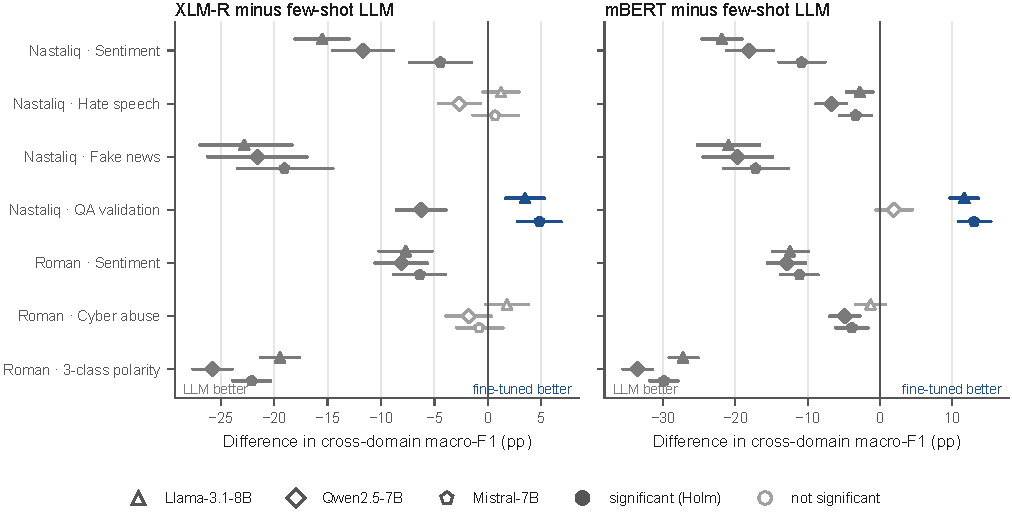
\includegraphics[width=\textwidth]{figures/forest.pdf}
\caption{Difference in mean cross-domain macro-F1 between each fine-tuned encoder and each LLM, with 95\% paired bootstrap confidence intervals (5{,}000 resamples). Filled markers: significant after Holm correction over all \val{boot.n} comparisons; orange: the LLM is better; blue: the fine-tuned encoder is better; open grey: not significant.}
\label{fig:forest}
\end{figure*}

\begin{table*}[t]\centering\scriptsize\setlength{\tabcolsep}{4pt}
\caption{Paired bootstrap comparison of mean cross-domain F1 (ST), fine-tuned encoder minus few-shot LLM, in pp with 95\% confidence intervals (5{,}000 resamples of test items per target, shared by both systems; fine-tuned predictions restricted to the LLM evaluation sample). Negative values favour the LLM. $^{*}$: Holm-adjusted $p<0.05$ over all \val{boot.n} comparisons.}
\label{tab:boot}\resizebox{\textwidth}{!}{\begin{tabular}{llccc}
\toprule
Matrix & Fine-tuned & $-$ Llama-3.1-8B & $-$ Qwen2.5-7B & $-$ Mistral-7B \\
\midrule
Sentiment & XLM-R & -15.5$^{*}$ [-18.0, -13.0] & -11.7$^{*}$ [-14.5, -8.8] & -4.4$^{*}$ [-7.3, -1.5] \\
 & mBERT & -21.9$^{*}$ [-24.6, -19.1] & -18.1$^{*}$ [-21.2, -14.7] & -10.8$^{*}$ [-14.0, -7.6] \\\addlinespace[2pt]
Hate Speech & XLM-R & +1.2 [-0.4, +2.9] & -2.7 [-4.6, -0.7] & +0.7 [-1.4, +2.8] \\
 & mBERT & -2.8$^{*}$ [-4.6, -0.9] & -6.7$^{*}$ [-8.8, -4.7] & -3.4$^{*}$ [-5.6, -1.2] \\\addlinespace[2pt]
Fake News & XLM-R & -22.8$^{*}$ [-26.9, -18.3] & -21.6$^{*}$ [-26.2, -16.9] & -19.0$^{*}$ [-23.4, -14.5] \\
 & mBERT & -20.9$^{*}$ [-25.2, -16.6] & -19.7$^{*}$ [-24.4, -14.8] & -17.2$^{*}$ [-21.7, -12.7] \\\addlinespace[2pt]
QA Validation & XLM-R & +3.5$^{*}$ [+1.7, +5.3] & -6.2$^{*}$ [-8.6, -3.9] & +4.8$^{*}$ [+2.8, +6.8] \\
 & mBERT & +11.7$^{*}$ [+9.7, +13.6] & +1.9 [-0.6, +4.5] & +13.0$^{*}$ [+10.9, +15.3] \\\addlinespace[2pt]
Sentiment (binary) & XLM-R & -7.7$^{*}$ [-10.2, -5.2] & -8.1$^{*}$ [-10.6, -5.7] & -6.4$^{*}$ [-8.8, -4.0] \\
 & mBERT & -12.4$^{*}$ [-14.9, -9.9] & -12.9$^{*}$ [-15.5, -10.3] & -11.1$^{*}$ [-13.7, -8.6] \\\addlinespace[2pt]
Cyber Abuse & XLM-R & +1.8 [-0.2, +3.8] & -1.8 [-3.9, +0.3] & -0.8 [-2.9, +1.4] \\
 & mBERT & -1.3 [-3.4, +0.8] & -4.9$^{*}$ [-7.0, -2.8] & -3.9$^{*}$ [-6.1, -1.7] \\\addlinespace[2pt]
3-class Polarity & XLM-R & -19.4$^{*}$ [-21.2, -17.7] & -25.8$^{*}$ [-27.6, -24.0] & -22.1$^{*}$ [-23.9, -20.3] \\
 & mBERT & -27.2$^{*}$ [-29.1, -25.2] & -33.5$^{*}$ [-35.5, -31.5] & -29.9$^{*}$ [-31.8, -27.9] \\
\bottomrule
\end{tabular}
}
\end{table*}

\paragraph{Are low LLM scores a prompting artefact?} Parse failures are rare (Table~\ref{tab:parse}): at most \val{pf.nonmistralmax}\% of items for Llama-3.1-8B and Qwen2.5-7B in any matrix. Mistral-7B is the exception on the two binary sentiment matrices, with \val{pf.N-SA.Mistral-7B}\% (Nastaliq) and \val{pf.R-SA.Mistral-7B}\% (Roman) unparseable outputs. These outputs are almost all ``Neutral'', often followed by a justification: the model declines to choose between the two allowed labels rather than producing malformed text. They count as errors, so Mistral-7B's sentiment scores are a lower bound for this prompt. Elsewhere, low LLM scores are not caused by unparseable outputs.

\begin{table}[t]\centering\small
\caption{LLM parse-failure rate (\% of all evaluated items, over all shifts and demonstration draws): outputs that name none of the allowed labels. They are scored as errors.}
\label{tab:parse}\resizebox{\columnwidth}{!}{\begin{tabular}{lrrr}
\toprule
Matrix & Llama-3.1-8B & Qwen2.5-7B & Mistral-7B \\
\midrule
Sentiment (N) & 0.03 & 0.32 & 8.02 \\
Hate Speech (N) & 0.00 & 0.00 & 0.02 \\
Fake News (N) & 0.00 & 0.00 & 0.00 \\
QA Validation (N) & 0.00 & 0.00 & 0.00 \\
Sentiment (binary) (R) & 0.07 & 0.12 & 4.54 \\
Cyber Abuse (R) & 0.00 & 0.00 & 0.00 \\
3-class Polarity (R) & 0.15 & 0.00 & 0.00 \\
\bottomrule
\end{tabular}
}
\end{table}

\subsection{Label granularity: binary versus three-class polarity}\label{sec:granularity}
Roman Sentiment and Roman 3-class polarity are the same task type with different label sets, and the label set accounts for much of the difference between their scores. The random baseline is \val{R-SA.rand} for the binary matrix and \val{R-P3.rand} for the three-class matrix. XLM-R scores SS \val{R-SA.XLM-R.SS} on binary sentiment against \val{R-P3.XLM-R.SS} on three-class polarity, and its mean Source Drop rises from \val{R-SA.XLM-R.dS} to \val{R-P3.XLM-R.dS} pp. The LLMs, whose in-domain scores fall by a similar amount, keep their Source Drop small in both matrices (\val{range.R-SA.llm.dS} and \val{range.R-P3.llm.dS} pp).

Inside the three-class matrix, the collection of origin matters as much as the label set. XLM-R reaches a mean ST of \val{R-P3.XLM-R.withinTW} on shifts between the three generated opinion domains, \val{R-P3.XLM-R.across} between reviews and opinions, and \val{R-P3.XLM-R.withinPR} between the three organic review domains. The generated opinion domains share a generator and transfer well among themselves; the organic review domains (e-commerce, restaurants and general comments) differ in platform, class balance and the amount of English, and transfer worst. The LLMs show the same order (Qwen2.5-7B: \val{R-P3.Qwen2.5-7B.withinTW}, \val{R-P3.Qwen2.5-7B.across} and \val{R-P3.Qwen2.5-7B.withinPR}) at a higher level.

\subsection{Organic-only analysis (RQ4)}\label{sec:organic}
Table~\ref{tab:organic} repeats the analysis on the organic submatrices. Nastaliq sentiment (one organic domain) and Roman cyber abuse (none) drop out; fake news and Roman binary sentiment are organic throughout and are unchanged. The answer to RQ2 holds: in every remaining matrix the fine-tuned encoders retain less of their in-domain score than the LLMs, except in QA, where Llama-3.1-8B retains only \val{org.N-QA.Llama-3.1-8B.rob}\% (ST \val{org.N-QA.Llama-3.1-8B.ST}). Fake news remains the matrix with the lowest fine-tuned retention (\val{org.N-FN.XLM-R.rob}\% for XLM-R) and binary sentiment the highest (\val{org.R-SA.XLM-R.rob}\%). One result changes. On its two organic domains, hate speech is no longer among the least robust matrices for fine-tuned models (\val{org.N-HS.XLM-R.rob}\% against \val{N-HS.XLM-R.rob}\% on all four domains), because its largest drops involve the generated HS-C and HS-D. Part of the low hate-speech robustness of the full matrix is thus a property of the generated domains.

\begin{table*}[t]\centering\small
\caption{Organic-only analysis: aggregates recomputed on the submatrix of organic domains (listed in brackets) for matrices with at least two. Symbols as in Table~\ref{tab:res-nsa}.}
\label{tab:organic}\resizebox{\textwidth}{!}{\begin{tabular}{llcccr}
\toprule
Matrix (organic domains) & Model & SS & ST & $\overline{\Delta_S}$ & \%Rob \\
\midrule
Hate Speech (HS-A, HS-B) & XLM-R & 0.811\,$\pm$\,0.008 & 0.591\,$\pm$\,0.004 & 21.9 & 73.0 \\
 & mBERT & 0.798\,$\pm$\,0.003 & 0.554\,$\pm$\,0.004 & 24.4 & 69.4 \\
 & Llama-3.1-8B & 0.628\,$\pm$\,0.050 & 0.622\,$\pm$\,0.013 & 0.6 & 99.4 \\
 & Qwen2.5-7B & 0.681\,$\pm$\,0.014 & 0.654\,$\pm$\,0.033 & 2.7 & 95.9 \\
 & Mistral-7B & 0.629\,$\pm$\,0.023 & 0.613\,$\pm$\,0.034 & 1.5 & 97.5 \\
\midrule
Fake News (FN-A, FN-B) & XLM-R & 0.782\,$\pm$\,0.119 & 0.356\,$\pm$\,0.030 & 42.6 & 45.9 \\
 & mBERT & 0.860\,$\pm$\,0.008 & 0.384\,$\pm$\,0.005 & 47.6 & 44.7 \\
 & Llama-3.1-8B & 0.605\,$\pm$\,0.061 & 0.581\,$\pm$\,0.022 & 2.4 & 96.4 \\
 & Qwen2.5-7B & 0.570\,$\pm$\,0.054 & 0.569\,$\pm$\,0.021 & 0.1 & n/a$^\dagger$ \\
 & Mistral-7B & 0.509\,$\pm$\,0.042 & 0.543\,$\pm$\,0.023 & -3.5 & n/a$^\dagger$ \\
\midrule
QA Validation (QA-A, QA-B) & XLM-R & 0.928\,$\pm$\,0.006 & 0.605\,$\pm$\,0.037 & 32.3 & 65.2 \\
 & mBERT & 0.932\,$\pm$\,0.006 & 0.672\,$\pm$\,0.015 & 26.0 & 72.1 \\
 & Llama-3.1-8B & 0.655\,$\pm$\,0.032 & 0.390\,$\pm$\,0.032 & 26.5 & 59.7 \\
 & Qwen2.5-7B & 0.737\,$\pm$\,0.014 & 0.605\,$\pm$\,0.057 & 13.3 & 82.0 \\
 & Mistral-7B & 0.610\,$\pm$\,0.017 & 0.502\,$\pm$\,0.057 & 10.8 & 82.5 \\
\midrule
Sentiment (binary) (SA-A, SA-B, SA-C) & XLM-R & 0.855\,$\pm$\,0.000 & 0.720\,$\pm$\,0.005 & 13.5 & 84.2 \\
 & mBERT & 0.850\,$\pm$\,0.003 & 0.682\,$\pm$\,0.009 & 16.8 & 80.2 \\
 & Llama-3.1-8B & 0.818\,$\pm$\,0.011 & 0.798\,$\pm$\,0.006 & 2.0 & 97.5 \\
 & Qwen2.5-7B & 0.817\,$\pm$\,0.015 & 0.802\,$\pm$\,0.007 & 1.5 & 98.2 \\
 & Mistral-7B & 0.798\,$\pm$\,0.021 & 0.785\,$\pm$\,0.023 & 1.3 & 98.3 \\
\midrule
3-class Polarity (PR-A, PR-B, PR-D) & XLM-R & 0.592\,$\pm$\,0.003 & 0.380\,$\pm$\,0.005 & 21.2 & 64.2 \\
 & mBERT & 0.615\,$\pm$\,0.013 & 0.367\,$\pm$\,0.006 & 24.8 & 59.7 \\
 & Llama-3.1-8B & 0.616\,$\pm$\,0.021 & 0.581\,$\pm$\,0.006 & 3.4 & 94.5 \\
 & Qwen2.5-7B & 0.627\,$\pm$\,0.018 & 0.587\,$\pm$\,0.008 & 4.1 & 93.6 \\
 & Mistral-7B & 0.624\,$\pm$\,0.013 & 0.578\,$\pm$\,0.013 & 4.6 & 92.7 \\
\bottomrule
\end{tabular}
}
\end{table*}

\subsection{Nastaliq versus Roman Urdu}\label{sec:script}
The two tracks share only two task types (sentiment and abusive language) and differ in sources and registers, so script effects cannot be separated from source effects, and we compare them only descriptively. For sentiment, fine-tuned retention is \val{range.N-SA.ft.rob}\% in Nastaliq and \val{range.R-SA.ft.rob}\% in Roman Urdu. For abusive language it is lower in Nastaliq (\val{range.N-HS.ft.rob}\%) than in Roman Urdu (\val{range.R-CA.ft.rob}\%), but the Nastaliq matrix combines two organic tweet corpora with two generated domains that label mild criticism as hateful (Section~\ref{sec:errors}), while three of the four Roman domains are generated with a shared style. These data do not support a claim that either script is harder to transfer across.

\subsection{What causes the largest failures? (RQ3)}\label{sec:errors}
For each matrix we examine the \emph{worst-transferring shift}: the source$\rightarrow$target pair with the largest Target Drop for XLM-R, so that the target's own model does well and the failure cannot be attributed to a hard target. Figure~\ref{fig:conf} shows confusion matrices for that shift, and Table~\ref{tab:errcat} breaks down every XLM-R error on it. An item counts as an error when at least two of the three seeds misclassify it. Instead of labelling errors by hand, we measure three properties of each error and of each correctly classified item of the same target: whether its length lies outside the 5th--95th percentile of the source training split, whether more than half of its word types never occur in the source training split, and whether the target's own XLM-R also misclassifies it. A property that is much more frequent among errors than among correct items is a candidate explanation.

\begin{figure*}[p]
\centering
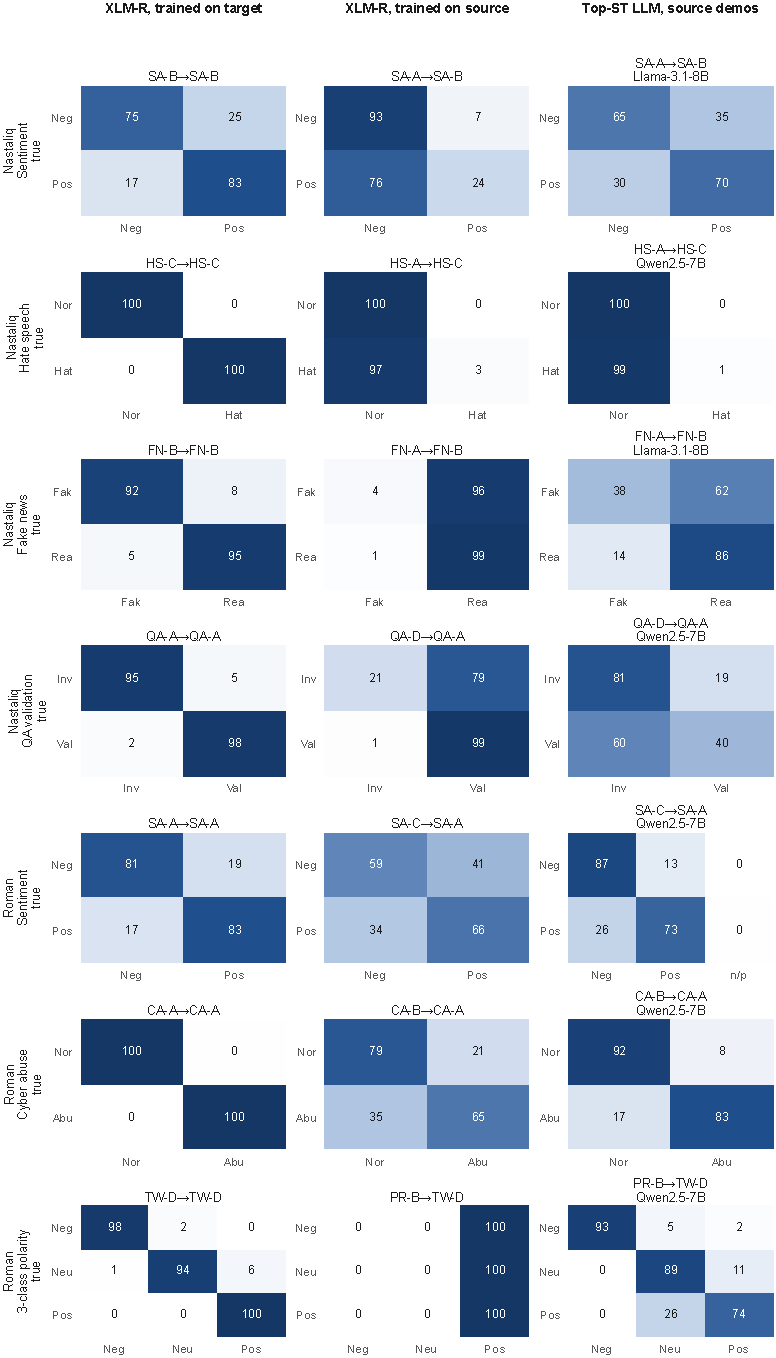
\includegraphics[width=0.8\textwidth]{figures/confusion_worst.pdf}
\caption{Confusion matrices (row-normalised, \%, summed over three seeds) for the worst-transferring shift of each matrix. Left: XLM-R trained on the target (in-domain reference). Middle: XLM-R trained on the source. Right: the few-shot LLM with the highest mean ST in the matrix, prompted with source demonstrations, on its evaluation sample; n/p = unparseable output. Darker cells hold more items.}
\label{fig:conf}
\end{figure*}

\begin{table*}[t]\centering\scriptsize\setlength{\tabcolsep}{3pt}
\caption{Measured breakdown of XLM-R errors on the worst-transferring shift of each matrix. Errors: items misclassified by at least two of three seeds, out of all test items of the target. Main confusion: most frequent true$\rightarrow$predicted pair and its share of errors. The last three columns give the percentage of errors (err) and of correctly classified items (ok) with each property: length outside the source's 5th--95th percentile; more than half of word types unseen in the source training data; also misclassified by the target's own XLM-R.}
\label{tab:errcat}\resizebox{\textwidth}{!}{\begin{tabular}{llccllll}
\toprule
Matrix & Shift & TT / ST & Errors & Main confusion (\%) & Length shift & Unseen vocab. & Hard in-domain \\
 & & & & & err / ok & err / ok & err / ok \\
\midrule
Sentiment (N) & SA-A$\rightarrow$SA-B & 0.79 / 0.51 & 663/1,638 & Positive$\rightarrow$Negative (93) & 100 / 100 & 3 / 1 & 22 / 17 \\
Hate Speech (N) & HS-A$\rightarrow$HS-C & 1.00 / 0.29 & 216/340 & Hate$\rightarrow$Normal (100) & 0 / 0 & 0 / 0 & 0 / 0 \\
Fake News (N) & FN-A$\rightarrow$FN-B & 0.94 / 0.38 & 772/1,645 & Fake$\rightarrow$Real (100) & 78 / 99 & 0 / 0 & 7 / 4 \\
QA Validation (N) & QA-D$\rightarrow$QA-A & 0.97 / 0.51 & 110/250 & Invalid$\rightarrow$Valid (100) & 100 / 100 & 99 / 100 & 5 / 1 \\
Sentiment (binary) (R) & SA-C$\rightarrow$SA-A & 0.82 / 0.63 & 773/2,140 & Negative$\rightarrow$Positive (50) & 22 / 16 & 49 / 45 & 29 / 11 \\
Cyber Abuse (R) & CA-B$\rightarrow$CA-A & 1.00 / 0.72 & 234/866 & Abusive$\rightarrow$Normal (66) & 20 / 21 & 44 / 48 & 0 / 0 \\
3-class Polarity (R) & PR-B$\rightarrow$TW-D & 0.97 / 0.17 & 213/320 & Negative$\rightarrow$Positive (52) & 0 / 0 & 95 / 83 & 5 / 0 \\
\bottomrule
\end{tabular}
}
\end{table*}

\paragraph{Collapse to one class.} In the worst shifts of three matrices the source model assigns one class to nearly every target item (Figure~\ref{fig:conf}). All \val{err.N-HS.nerr} errors of the HS-A model on HS-C are hate items labelled \emph{normal}; all \val{err.N-FN.nerr} errors of the FN-A model on FN-B are fake items labelled \emph{real}; and the PR-B model predicts \emph{positive} for every TW-D item. In two further matrices one class dominates the predictions: the Nastaliq tweet model labels most translated movie reviews \emph{negative}, and the QA-D model accepts most invalid QA-A pairs. For PR-B the training data explain the collapse, since 79\% of its items are positive. The few-shot LLM avoids the collapse in every case except hate speech, where it also labels almost all HS-C hate items as normal.

\paragraph{What the measured properties show.} Vocabulary and length rarely separate errors from correct items. In the sentiment, fake-news and QA shifts most target items lie outside the source's length range whether they are classified correctly or not, so length describes the whole target rather than the errors. In hate speech and cyber abuse, errors and correct items do not differ on either property. The one clear signal is in Roman binary sentiment, where \val{err.R-SA.hardin.err}\% of errors are also misclassified by the target's own model against \val{err.R-SA.hardin.ok}\% of correct items; many of these errors are items that are ambiguous or mislabelled in SA-A itself. Taken together, the worst failures reflect differences in what a label means and how often each class occurs, more than unfamiliar words.

\paragraph{Examples.} Table~\ref{tab:errex} shows misclassified items drawn at random from those that all three seeds get wrong and the target's own model gets right (six candidates per shift). None of the six sampled HS-C errors contains a slur, insult or threat: they are mild criticism of leaders, players or online behaviour, labelled hateful by the generated HS-C domain. Hateful HS-A tweets, such as the example in Table~\ref{tab:examples}, contain insults, so a model trained on HS-A, and an LLM given HS-A demonstrations, calls the HS-C items normal. The two domains share a label name but not a label definition. In fake news, the six sampled FN-B errors are short claims as they circulated on social media (a funeral presented as a protest, a map said to show a wrong border), whereas the fake items of FN-A are full fabricated articles of several hundred words written by journalists \citep{amjad2020bend}. A model that learned what a fabricated article looks like in FN-A has no basis for judging a one-line claim. The Roman sentiment and polarity examples are unambiguous complaints predicted as positive, and in cyber abuse a friendly CA-A comment with a misspelling and an emoticon (\textit{vidiyo}, \textit{:)}) is predicted abusive, which is consistent with the augmentation-like noise that led us to mark CA-A as uncertain.

\begin{table*}[t]\centering\small\renewcommand{\arraystretch}{1.3}
\caption{Misclassified items on the worst-transferring shifts (XLM-R, wrong for all three seeds, correct for the target's own model), with English glosses by the authors. Drawn at random (seed 0) from all items of at most 22 words that meet these conditions; the complete candidate list is released.}
\label{tab:errex}
\begin{tabular}{>{\raggedright\arraybackslash}p{2.2cm}>{\raggedright\arraybackslash}p{5.0cm}>{\raggedright\arraybackslash}p{3.9cm}>{\raggedright\arraybackslash}p{2.1cm}}
\toprule
Shift & Item & Gloss & Gold $\rightarrow$ pred. \\
\midrule
HS-A$\rightarrow$HS-C & \ur{حالیہ دنوں میں اس رہنما کے بیانات میں تضاد واضح ہے} & Lately, this leader's statements have been clearly contradictory. & Hate $\rightarrow$ Normal \\
HS-A$\rightarrow$HS-C & \ur{اکثر آن لائن ماحول میں برداشت کی کمی نظر آتی ہے} & Online spaces often show a lack of tolerance. & Hate $\rightarrow$ Normal \\
FN-A$\rightarrow$FN-B & \ur{دہلی میں این آر سی مخالف مظاہرے کے طور پر سلیمانی کا جنازہ نکلا۔} & Soleimani's funeral procession shown as an anti-NRC protest in Delhi. & Fake $\rightarrow$ Real \\
FN-A$\rightarrow$FN-B & \ur{ہندوستان کا وائرل نقشہ جموں و کشمیر کی غلط تقسیم کو ظاہر کرتا ہے۔} & India's viral map shows a wrong division of Jammu and Kashmir. & Fake $\rightarrow$ Real \\
SA-C$\rightarrow$SA-A & \textit{bhut bekar delivery ha} & The delivery is very bad. & Negative $\rightarrow$ Positive \\
CA-B$\rightarrow$CA-A & \textit{tera kontent bakwas hy bhai} & Your content is rubbish, brother. & Abusive $\rightarrow$ Normal \\
CA-B$\rightarrow$CA-A & \textit{Aray mujhe ye vidiyo pasand aaya :)} & Oh, I liked this video :) & Normal $\rightarrow$ Abusive \\
PR-B$\rightarrow$TW-D & \textit{Honestly app bar bar crash karti hai update ke baad bhi} & Honestly, the app keeps crashing even after the update. & Negative $\rightarrow$ Positive \\
\bottomrule
\end{tabular}
\end{table*}

% =====================================================================
\section{Limitations}\label{sec:limitations}
\begin{enumerate}[leftmargin=*,itemsep=2pt]
\item \textbf{Generated data.} \NumSynthDomains{} domains (\PctSynth\% of the benchmark) are LLM-generated, concentrated in hate speech, QA, cyber abuse and 3-class polarity. Cluster-aware splitting removes template leakage, but generated text carries a style signature that affects transfer: the generated opinion domains transfer well among themselves, in cyber abuse the label is partly predictable from length, and the shortcut audit shows that in HS-C the verb \ur{ہے} (``is'') occurs in \val{sc.N-HS.HS-C.in}\% of normal items against \val{sc.N-HS.HS-C.out}\% of hate items, a trace of how the two classes were generated. The organic-only analysis bounds these effects but cannot be run for Nastaliq sentiment or Roman cyber abuse. Generation prompts and the number of removed items were not recorded, and generated items were checked by one person.
\item \textbf{Provenance.} Three organic domains come from public uploads whose original authors could not be identified, so their annotation quality and licences are unverified.
\item \textbf{Fake news.} Only two fake-news domains meet the inclusion criteria, so this matrix has two shifts and its conclusions rest on one pair of corpora.
\item \textbf{Imbalanced domains.} Roman PR-B has 8 negative test items, so scores involving it are noisy; the per-target tables identify it.
\item \textbf{Models and prompts.} We test 7--8B LLMs in 4-bit precision with one prompt template, and encoders with one fixed set of hyperparameters; larger models, other prompts and tuned encoders may behave differently. Public organic corpora may also have been part of the LLMs' pretraining data, which would favour the LLMs on those domains.
\item \textbf{LLM evaluation sample.} LLMs are scored on up to 300 items per target domain; the bootstrap intervals quantify this uncertainty for the family comparison, but differences within a family are not tested.
\item \textbf{Error analysis.} The error categories are computed from the data, and the qualitative reading rests on a small random sample of examples rather than on a manual annotation of many errors.
\item \textbf{Two tracks, not a script comparison.} The scripts differ in sources and task coverage, so the tracks are not directly comparable.
\end{enumerate}

\section{Ethics statement}
The benchmark contains offensive, hateful and sectarian text collected from public online sources, released to support moderation research; releases carry content warnings. Automated hate-speech and fake-news classifiers can suppress legitimate speech, especially that of minorities, and should not be deployed without human review. Sectarian and ethnic hate in the Pakistani context is particularly sensitive, and models trained on these data could also be misused to probe moderation systems. Our observation that sampled items of a generated hate-speech domain label mild criticism of public figures as hateful is a further reason not to deploy a classifier trained on them. No crowd workers or external annotators were employed: all generated text, including generated hateful and abusive items, was read and checked by the first author, so questions of annotator compensation do not arise. Repeated exposure to such material is nevertheless a burden that future extensions with external annotators should plan for.

\section{Data statement}
Following \citet{bender2018data} and \citet{gebru2021datasheets}: \textbf{Language varieties:} Urdu in Perso-Arabic script (\texttt{urd-Arab}) and Roman Urdu (\texttt{urd-Latn}), mostly Pakistani usage, with frequent English code-mixing in the Roman track and some Punjabi in Nastaliq tweets. \textbf{Speakers:} authors of public tweets, YouTube comments, product and restaurant reviews, and news articles; generated text in \NumSynthDomains{} domains. \textbf{Annotation:} original corpus labels for organic data; labels for generated data were assigned in the generation prompt and checked by the first author, a native Urdu speaker. \textbf{Distribution:} GitHub (\repo), Zenodo (DOI \href{https://doi.org/10.5281/zenodo.23053495}{10.5281/zenodo.23053495}) and Hugging Face.

\section{Conclusion}
In conclusion, Urdu classifiers are far less robust to a change of data source than their in-domain scores suggest, and the English finding of \citet{calderon2024measuring} carries over to both Urdu scripts. Fine-tuned XLM-R and mBERT are the stronger in-domain classifiers in \val{all.ftSSwins} of \NumMatrices{} matrices but lose \val{all.ft.dSmin}--\val{all.ft.dSmax} pp of macro-F1 on another domain, and in most shifts they do worse than a model trained on the target, so the loss is a robustness failure rather than a move to a harder domain. Few-shot LLMs lose much less and are significantly stronger across domains in \val{boot.llmbetter} of \val{boot.n} comparisons. The exceptions are informative: fine-tuning transfers better in QA validation, neither family transfers usefully in fake news, and the largest failures of both families occur where two domains attach the same label to different kinds of text, a problem that robustness to vocabulary or spelling would not solve. Reaching these conclusions required choosing domains by explicit criteria. Duplicated domains, labels that follow the origin of an item, question-level overlap and template near-duplicates each change cross-domain scores, and we recommend the audits released with this benchmark to anyone combining public and generated corpora into a multi-domain evaluation.

\section*{Acknowledgments}
We thank the FAST School of Computing, FAST-NUCES Lahore, for computing facilities, and the creators of the public corpora this benchmark builds on.

\bibliographystyle{plainnat}
\bibliography{refs}

\onecolumn
\appendix
\section{Evidence of LLM generation in each domain}\label{app:synth}
This appendix supports the origin labels in Table~\ref{tab:datasets}. For every candidate domain it reports three signals that separate LLM-generated from human-written text in our data: templated near-duplicates, lexical diversity and the variability of item length (Section~\ref{sec:collection}).
\begin{table}[H]\centering\scriptsize
\caption{Generation signals for all \NumDomainsVten{} candidate domains (train and test pooled). Template\,\%: items with a near-duplicate variant (character 5-gram Jaccard $\geq 0.8$) inside the domain. Distinct-2: distinct word bigrams per bigram in a 500-item sample. Len.\,CV: coefficient of variation of item length in words. Seed\,\%: items near-duplicating an item of another domain of the same script. QA items are question--answer pairs, whose shared questions raise Template\,\% by construction.}
\label{tab:synth-audit}
\resizebox{\textwidth}{!}{\begin{tabular}{llrrrrrl}
\toprule
Domain & Name & $N$ & Template\,\% & Distinct-2 & Len.\,CV & Seed\,\% & Origin \\
\midrule
Nas SA-A & Twitter Social Media & 979 & 1.6 & 0.89 & 0.41 & 100.0 & organic \\
Nas SA-B & Movie Reviews & 9,163 & 0.3 & 0.47 & 0.82 & 8.9 & translated \\
Nas SA-C & Civic Social Topics & 162 & 0.0 & 0.73 & 0.15 & 0.0 & excluded \\
Nas SA-D & Governance Political & 978 & 1.4 & 0.88 & 0.41 & 100.0 & excluded \\
Nas SA-E & Socioeconomic Agricultural & 2,382 & 59.6 & 0.21 & 0.15 & 0.0 & generated \\
Nas HS-A & Social Media Offensive & 21,631 & 4.8 & 0.85 & 0.60 & 100.0 & organic \\
Nas HS-B & Social Media Hate Speech & 24,927 & 27.4 & 0.85 & 0.67 & 0.1 & organic \\
Nas HS-C & Politics Sports Health Family & 1,700 & 27.7 & 0.18 & 0.15 & 1.3 & generated \\
Nas HS-D & Sports Labor Arts Education & 1,700 & 41.2 & 0.24 & 0.17 & 0.3 & generated \\
Nas HS-E & Inter Faith Sectarian Ethnic & 21,629 & 4.8 & 0.83 & 0.60 & 100.0 & excluded \\
Nas FN-A & Multi Topic News & 899 & 2.9 & 0.45 & 0.75 & 37.8 & organic \\
Nas FN-B & Ax to Grind & 9,812 & 13.0 & 0.65 & 1.98 & 4.5 & organic \\
Nas FN-C & General Pakistani News & 23,171 & 0.3 & 0.79 & 0.30 & 0.2 & excluded \\
Nas FN-D & Fact Checking Platform & 13,388 & 0.4 & 0.55 & 0.46 & 0.0 & excluded \\
Nas QA-A & Religious Hadith & 1,580 & 50.8 & 0.29 & 0.52 & 0.0 & organic \\
Nas QA-B & General Knowledge & 11,306 & 21.3 & 0.44 & 0.33 & 0.0 & organic \\
Nas QA-C & Long Form QnA & 1,120 & 51.8 & 0.10 & 0.09 & 0.0 & generated \\
Nas QA-D & Short Form QnA & 3,460 & 23.2 & 0.29 & 0.17 & 0.0 & generated \\
Rom CA-A & YouTube Comments & 4,868 & 25.9 & 0.56 & 0.29 & 6.4 & uncertain \\
Rom CA-B & Content Creator Comments & 1,300 & 67.5 & 0.29 & 0.18 & 0.0 & generated \\
Rom CA-C & Social Media Diverse Vocab & 1,300 & 63.2 & 0.32 & 0.17 & 0.0 & generated \\
Rom CA-D & General Online Video & 1,200 & 53.3 & 0.23 & 0.22 & 19.6 & generated \\
Rom PR-A & Daraz Ecommerce & 16,944 & 2.9 & 0.82 & 0.92 & 0.5 & organic \\
Rom PR-B & Restaurant Food & 750 & 0.5 & 0.74 & 0.65 & 0.4 & organic \\
Rom PR-D & Electronics Gaming Delivery & 26,666 & 23.2 & 0.93 & 1.10 & 2.8 & organic \\
Rom SA-A & Mixed Public Discourse & 21,444 & 0.5 & 0.95 & 0.98 & 2.8 & organic \\
Rom SA-B & Social Media Politics Drama & 10,993 & 1.6 & 0.89 & 1.18 & 100.0 & organic \\
Rom SA-C & YouTube Entertainment & 20,070 & 6.0 & 0.94 & 0.98 & 1.1 & organic \\
Rom SA-D & Utilities Apps Courses & 10,993 & 1.6 & 0.89 & 1.18 & 100.0 & excluded \\
Rom TW-A & Twitter Political Social & 17,884 & 1.0 & 0.91 & 1.27 & 61.8 & excluded \\
Rom TW-B & Consumer Electronics Gaming & 1,450 & 93.2 & 0.18 & 0.15 & 0.0 & generated \\
Rom TW-C & Public Civic Services & 1,450 & 91.9 & 0.19 & 0.13 & 0.0 & generated \\
Rom TW-D & Mixed Social Commentary & 1,600 & 92.4 & 0.23 & 0.12 & 0.0 & generated \\
\bottomrule
\end{tabular}
}
\end{table}

\clearpage
\section{Does a single phrase reveal the label?}\label{app:shortcuts}
This appendix supports the second inclusion criterion (Section~\ref{sec:criteria}). For each included domain it shows the phrase whose frequency differs most between classes. A content word is expected; a dateline, byline or other source marker would mean that the label can be read off the origin of an item.
\begin{table}[H]\centering\scriptsize
\caption{For every included domain, the word n-gram ($n\leq3$, at least 20 occurrences) with the largest difference in document frequency between one class and the others. Content words are expected; source boilerplate (datelines, bylines) would indicate that the label follows the origin of an item.}
\label{tab:shortcuts}
\begin{tabular}{lllcrr}
\toprule
Matrix & Domain & Phrase & Class & \% of class & \% of others \\
\midrule
Sentiment (N) & SA-A & \ur{پر} & Negative & 17.1 & 9.0 \\
Sentiment (N) & SA-B & \ur{خراب} & Negative & 26.4 & 7.5 \\
Sentiment (N) & SA-E & \ur{دیا} & Negative & 45.3 & 4.7 \\
Hate Speech (N) & HS-A & \ur{کو} & Hate & 38.9 & 30.1 \\
Hate Speech (N) & HS-B & \ur{میں} & Normal & 34.8 & 24.8 \\
Hate Speech (N) & HS-C & \ur{ہے} & Normal & 97.3 & 44.7 \\
Hate Speech (N) & HS-D & \ur{صرف} & Hate & 28.0 & 0.0 \\
Fake News (N) & FN-A & \ur{ہے۔} & Real & 41.8 & 25.3 \\
Fake News (N) & FN-B & \ur{نہیں} & Fake & 32.6 & 9.8 \\
QA Validation (N) & QA-A & \ur{وہ} & Invalid & 39.8 & 33.3 \\
QA Validation (N) & QA-B & \ur{ہے} & Valid & 52.0 & 50.9 \\
QA Validation (N) & QA-C & \ur{پیدا} & Valid & 12.9 & 9.1 \\
QA Validation (N) & QA-D & \ur{ہے} & Valid & 30.3 & 27.7 \\
Sentiment (binary) (R) & SA-A & \textit{ha} & Positive & 19.8 & 12.9 \\
Sentiment (binary) (R) & SA-B & \textit{ko} & Negative & 31.8 & 17.6 \\
Sentiment (binary) (R) & SA-C & \textit{baap} & Negative & 16.9 & 0.1 \\
Cyber Abuse (R) & CA-A & \textit{hai} & Abusive & 22.1 & 10.7 \\
Cyber Abuse (R) & CA-B & \textit{nahi} & Abusive & 27.8 & 3.1 \\
Cyber Abuse (R) & CA-C & \textit{nahi} & Abusive & 30.1 & 0.0 \\
Cyber Abuse (R) & CA-D & \textit{hai} & Abusive & 72.6 & 33.3 \\
3-class Polarity (R) & PR-A & \textit{but} & Neutral & 53.3 & 6.7 \\
3-class Polarity (R) & PR-B & \textit{quality} & Negative & 35.7 & 11.5 \\
3-class Polarity (R) & PR-D & \textit{allah} & Positive & 12.9 & 2.7 \\
3-class Polarity (R) & TW-B & \textit{raha} & Negative & 27.3 & 4.1 \\
3-class Polarity (R) & TW-C & \textit{nahi} & Negative & 55.7 & 2.3 \\
3-class Polarity (R) & TW-D & \textit{nahi} & Negative & 52.3 & 8.5 \\
\bottomrule
\end{tabular}

\end{table}

\clearpage
\section{Source, URL and licence of each domain}\label{app:prov}
This appendix lists where each domain comes from, how its origin was confirmed, and the licence under which it is distributed (Section~\ref{sec:licensing}).
\begin{table}[H]\centering\scriptsize
\caption{Source and licence of every domain. Verified: our files were matched against the public release (content or file identity). Untraced: obtained from a public upload whose original author could not be identified. Generated: produced by the first author with xAI Grok (Section~\ref{sec:collection}).}
\label{tab:provenance}
\resizebox{\textwidth}{!}{\begin{tabular}{llp{1.3cm}p{5.0cm}p{5.6cm}p{2.4cm}}
\toprule
Domain & Origin & Source & Description & URL & Licence \\
\midrule
Nas SA-A & organic & verified & Urdu Sentiment Corpus v1.0 (Khan \& Nizami 2020) \citep{khan2020usc} & \url{https://github.com/MuhammadYaseenKhan/Urdu-Sentiment-Corpus} & none stated (citation requested) \\
Nas SA-B & translated & verified & IMDB reviews machine-translated into Urdu (Hugging Face upload by mirfan899); 91\% of items match after normalising punctuation and letter variants \citep{mirfan899imdb} & \url{https://huggingface.co/datasets/mirfan899/imdb_urdu_reviews} & ODbL 1.0 \\
Nas SA-E & generated & generated & Grok-generated by first author & -- & xAI terms (attribute Grok) \\
Nas HS-A & organic & verified & ISE-Hate corpus (Akram, Shahzad \& Bashir 2023); same 21,361 tweets, 98.7\% label agreement with Level-1 \citep{akram2023isehate} & \url{https://github.com/hammad7007/ISE_dataset} & none stated \\
Nas HS-B & organic & verified & Urdu hate-speech tweets (Hugging Face upload by Adnan855570); our raw file is byte-identical \citep{adnan2025urduhate} & \url{https://huggingface.co/datasets/Adnan855570/Urdu_Hate_Speech} & MIT \\
Nas HS-C & generated & generated & Grok-generated by first author & -- & xAI terms (attribute Grok) \\
Nas HS-D & generated & generated & Grok-generated by first author & -- & xAI terms (attribute Grok) \\
Nas FN-A & organic & verified & Bend the Truth (Amjad et al. 2020) \citep{amjad2020bend} & \url{https://github.com/MaazAmjad/Datasets-for-Urdu-news} & none stated \\
Nas FN-B & organic & verified & Ax-to-Grind Urdu (Harris et al. 2023) \citep{harris2023axtogrind} & \url{https://github.com/HjH-Whu-CRC/Ax-to-Grind-Urdu} & none stated \\
Nas QA-A & organic & verified & mirfan899/Urdu GitHub collection (MIT); 100\% content match \citep{mirfan899urdu} & \url{https://github.com/mirfan899/Urdu} & MIT \\
Nas QA-B & organic & verified & mirfan899/Urdu GitHub collection (MIT); 100\% content match \citep{mirfan899urdu} & \url{https://github.com/mirfan899/Urdu} & MIT \\
Nas QA-C & generated & generated & Grok-generated by first author (70 questions x 8 variants) & -- & xAI terms (attribute Grok) \\
Nas QA-D & generated & generated & Grok-generated by first author & -- & xAI terms (attribute Grok) \\
\midrule
Rom SA-A & organic & verified & HF ayeshasameer/roman-urdu-sentiment-analysis (MIT); identical test split \citep{ayeshasameer2024romanurdu} & \url{https://huggingface.co/datasets/ayeshasameer/roman-urdu-sentiment-analysis} & MIT \\
Rom SA-B & organic & verified & RUSAD (Mehmood Essam \& Shafi 2019) \citep{mehmood2019rusad} & \url{https://archive.ics.uci.edu/dataset/854/roman+urdu+sentiment+analysis+dataset+(rusad)} & CC BY 4.0 \\
Rom SA-C & organic & untraced & YouTube comments; uploader unknown & -- & unknown \\
Rom CA-A & uncertain & untraced & Unknown; shows augmentation noise & -- & unknown \\
Rom CA-B & generated & generated & Grok-generated by first author & -- & xAI terms (attribute Grok) \\
Rom CA-C & generated & generated & Grok-generated by first author & -- & xAI terms (attribute Grok) \\
Rom CA-D & generated & generated & Grok-generated by first author (seeds partly from CA-A: 20\% near-matches) & -- & xAI terms (attribute Grok) \\
Rom PR-A & organic & verified & Daraz Code-Mixed Product Reviews (Kaggle) \citep{daraz2023kaggle} & \url{https://www.kaggle.com/datasets/yrrebeere/daraz-code-mixed-product-reviews} & CC BY 4.0 \\
Rom PR-B & organic & untraced & Kababjees restaurant reviews & -- & unknown \\
Rom PR-D & organic & verified & RUWV-NSR, Soomro et al. 2024 Data in Brief; identical file name and byte size \citep{soomro2024ruwv} & \url{https://data.mendeley.com/datasets/v5jfhsvtmd/4} & CC BY 4.0 \\
Rom TW-B & generated & generated & Grok-generated by first author & -- & xAI terms (attribute Grok) \\
Rom TW-C & generated & generated & Grok-generated by first author & -- & xAI terms (attribute Grok) \\
Rom TW-D & generated & generated & Grok-generated by first author & -- & xAI terms (attribute Grok) \\
\bottomrule
\end{tabular}
}
\end{table}

\clearpage
\section{Prompt used for the few-shot LLMs}\label{app:prompt}
The user message sent to every LLM, before the model's chat template is applied. \texttt{<INSTRUCTION>} is ``Classify the sentiment of the text.'', ``Decide whether the text is abusive or hateful.'', ``Decide whether the news text is real or fake.'' or ``Decide whether the answer is a valid answer to the question.''; \texttt{<SCRIPT>} is ``Nastaliq (Perso-Arabic) script'' or ``Roman (Latin) script''; \texttt{<LABELS>} lists the label words of the matrix (e.g.\ ``Negative or Positive'', ``Negative, Neutral or Positive''). Each demonstration and the test item are rendered as \texttt{Text: \dots}, or as \texttt{Question: \dots} and \texttt{Answer: \dots} lines for QA, followed by \texttt{Label:}.
\begin{verbatim}
<INSTRUCTION> The text is Urdu written in <SCRIPT>. Answer with exactly
one word: <LABELS>.

Examples:

Text: <demonstration 1>
Label: <label 1>

... (5 demonstrations per class, shuffled)

Now classify:

Text: <test item>
Label:
\end{verbatim}

\end{document}
